\documentclass[11pt]{article}
\usepackage[utf8]{inputenc}
\usepackage{amsmath}
\usepackage{natbib}
\usepackage{graphicx}
%\usepackage[spanish, es-minimal]{babel}
\usepackage[spanish, es-minimal, english]{babel}
%\usepackage[vmargin=0.8in, hmargin=1.00in]{geometry}
\usepackage[vmargin=0.7in, hmargin=1.0in]{geometry}
\usepackage{lipsum}

\newcommand\U[1]{\ensuremath{\mathrm{#1}}}
\newcommand\K{\U{K}}
\newcommand\cm{\U{cm}}
\newcommand\AU{\U{AU}}
\newcommand\g{\U{g}}
\newcommand\msolagno{M_\odot\,\U{yr^{-1}}}

\newcommand\acre{\ensuremath{_{\mathrm{acre}}}}
\newcommand\eff{\ensuremath{_{\mathrm{eff}}}}
\newcommand\Ext{\ensuremath{_{\mathrm{Ext}}}}
\newcommand\Int{\ensuremath{_{\mathrm{Int}}}}

\newcommand\BowshockFig[1]{
  \includegraphics[width=\figwidth, clip, trim=10 10 10 10]
  {#1}
}
\newcommand\raiselabel[1]{\raisebox{0.9\figwidth}[-0.5\figwidth]{#1}}
\newcommand\raiselabelPho[1]{\raisebox{0.62\figwidth}[-0.5\figwidth]{#1}}



\title{SMC planetary nenubae in S-PLUS }

%\author{
   %Bolsista: Luis Angel Gutiérrez Soto\\
   %Coordenadora: Claudia Lucia Mendes de Oliveira 
%}
\date{}

\begin{document}
\maketitle

\section{Science verification}
\label{sec:ini}

\begin{figure}
\centering
\begin{tabular}{l l}
  \includegraphics[width=0.52\linewidth, trim=10 15 5 8, clip]{../../Dropbox/JPAS/Tesis/Fig/DdDm-1-HPNe-SPLUS18-magnitude-paper.pdf}
   \includegraphics[width=0.5\linewidth, trim=5 15 5 8, clip]{../../Dropbox/JPAS/Tesis/Fig/DdDm1_L4_T200_output_SED-tere_E02_600-JPLUS17-magnitude-paper.pdf}
  \end{tabular}  
\end{figure}



\begin{figure}[!h]
  \includegraphics[width=0.5\linewidth, trim=10 10 10 10, clip]{../../Dropbox/JPAS/Tesis/Fig/Fig1-JPLUS17-Viironen.pdf}
\end{figure}

\begin{figure*}[1h]
%\setlength\tabcolsep{\figstampcolsep}
\centering
\begin{tabular}{l l}
 \includegraphics[width=0.5\linewidth, trim=10 10 10 10, clip]{../../Dropbox/JPAS/Tesis/Fig/Fig2-JPLUS17-J0515-J0660.pdf} & \includegraphics[width=0.5\linewidth, trim=10 10 10 10, clip]{../../Dropbox/JPAS/Tesis/Fig/Fig5-JPLUS17-J0660-r.pdf} \\
%\raiselabel{(\textit{a})} & \raiselabel{(\textit{b})}\\
\includegraphics[width=0.5\linewidth, trim=10 10 10 10, clip]{../../Dropbox/JPAS/Tesis/Fig/Fig3-JPLUS17-z-g.pdf} & \includegraphics[width=0.5\linewidth, trim=10 10 10 10, clip]{../../Dropbox/JPAS/Tesis/Fig/Fig6-JPLUS17-g-i.pdf} \\
%\raiselabel{(\textit{c})} & \raiselabel{(\textit{d})}
  
  \end{tabular}
\end{figure*}

I found this sample of SMC PNe: vizier-> J/A+A/472/101/table7. Chemical evolution of SMC planetary nebulae (Idiart+, 2007, 2007A\&A…472..101I) This catalog has $\sim$40 PNe.\\

I made cross matching between this catalog and SPLUS catalog. I found 21 matches using a 1 arcsec of radii. 

I put the final matches in my diagram,


\begin{figure}[!h]
  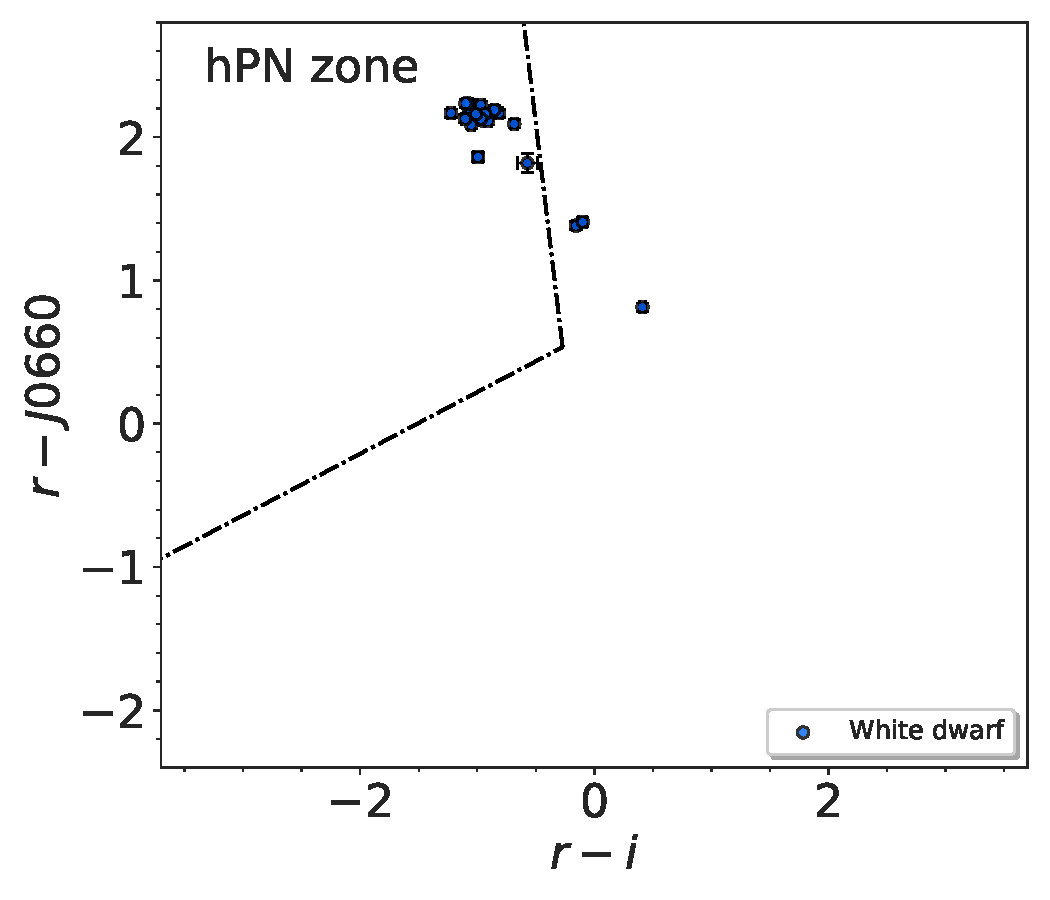
\includegraphics[width=0.5\linewidth, trim=10 10 10 10, clip]{Fig1-IDR2-SPLUS-vironen.pdf}
\end{figure}

\begin{figure*}[1h]
%\setlength\tabcolsep{\figstampcolsep}
\centering
\begin{tabular}{l l}
 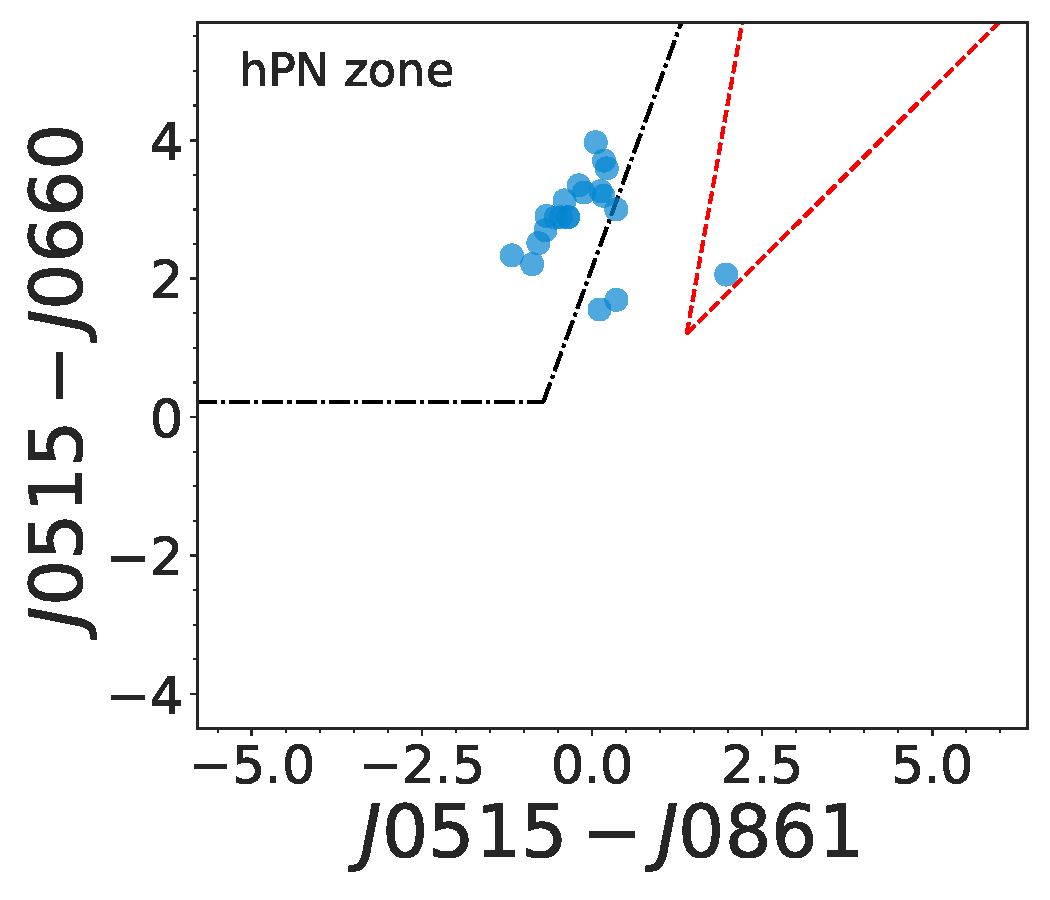
\includegraphics[width=0.5\linewidth, trim=10 10 10 10, clip]{Fig2-IDR2-SPLUS-J0515_J0660.pdf} & 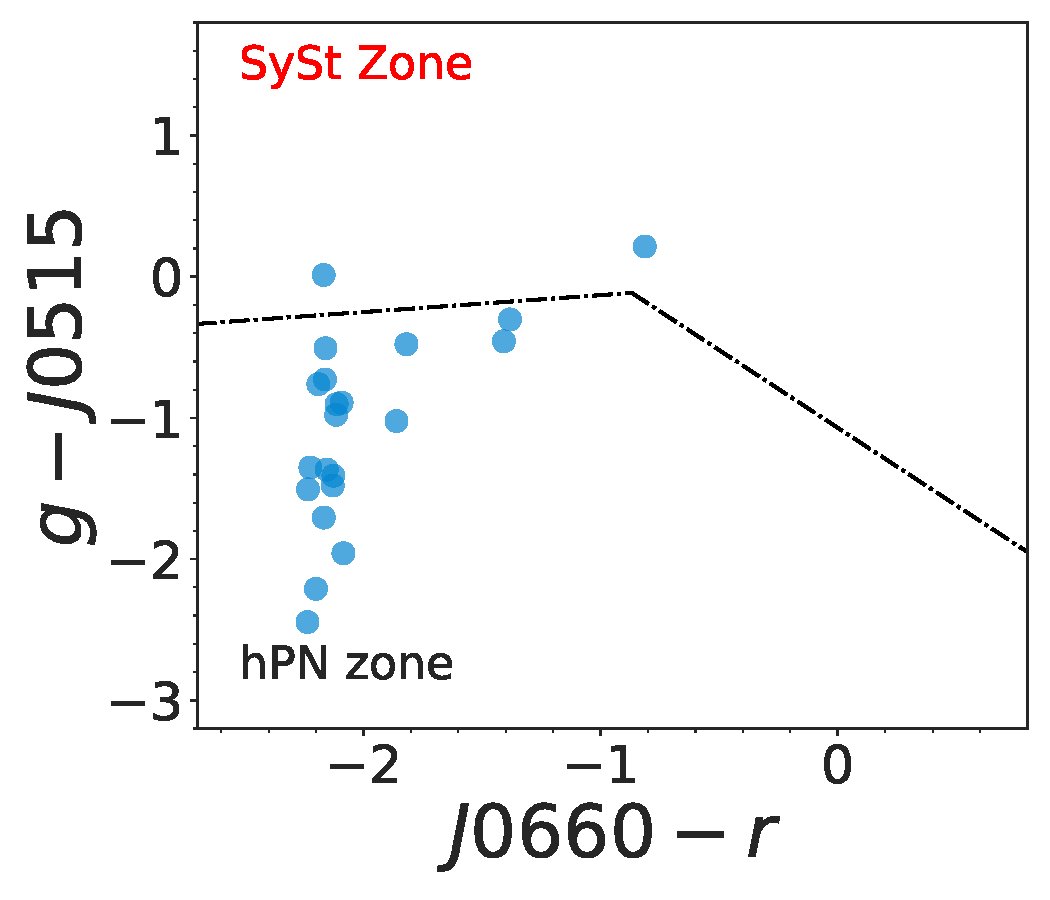
\includegraphics[width=0.5\linewidth, trim=10 10 10 10, clip]{Fig4-IDR2-SPLUS-g.pdf} \\
%\raiselabel{(\textit{a})} & \raiselabel{(\textit{b})}\\
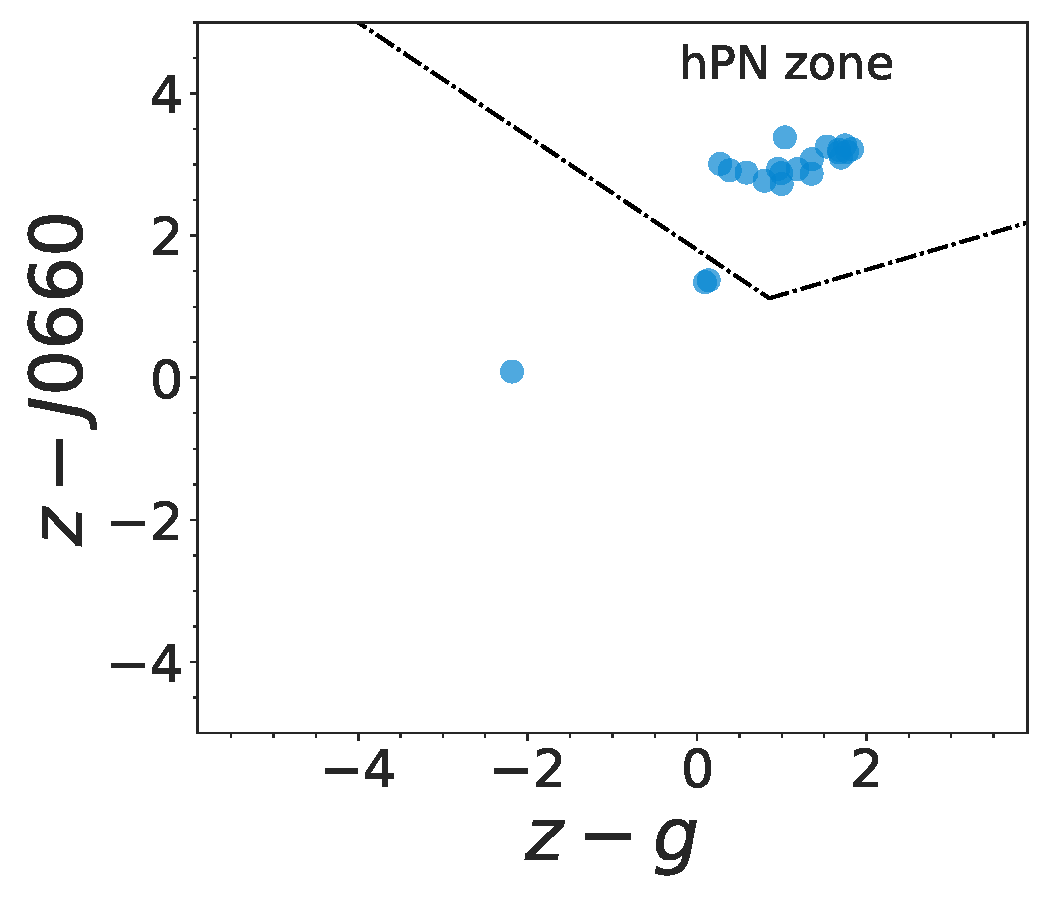
\includegraphics[width=0.5\linewidth, trim=10 10 10 10, clip]{Fig3-IDR2-SPLUS-z.pdf} & 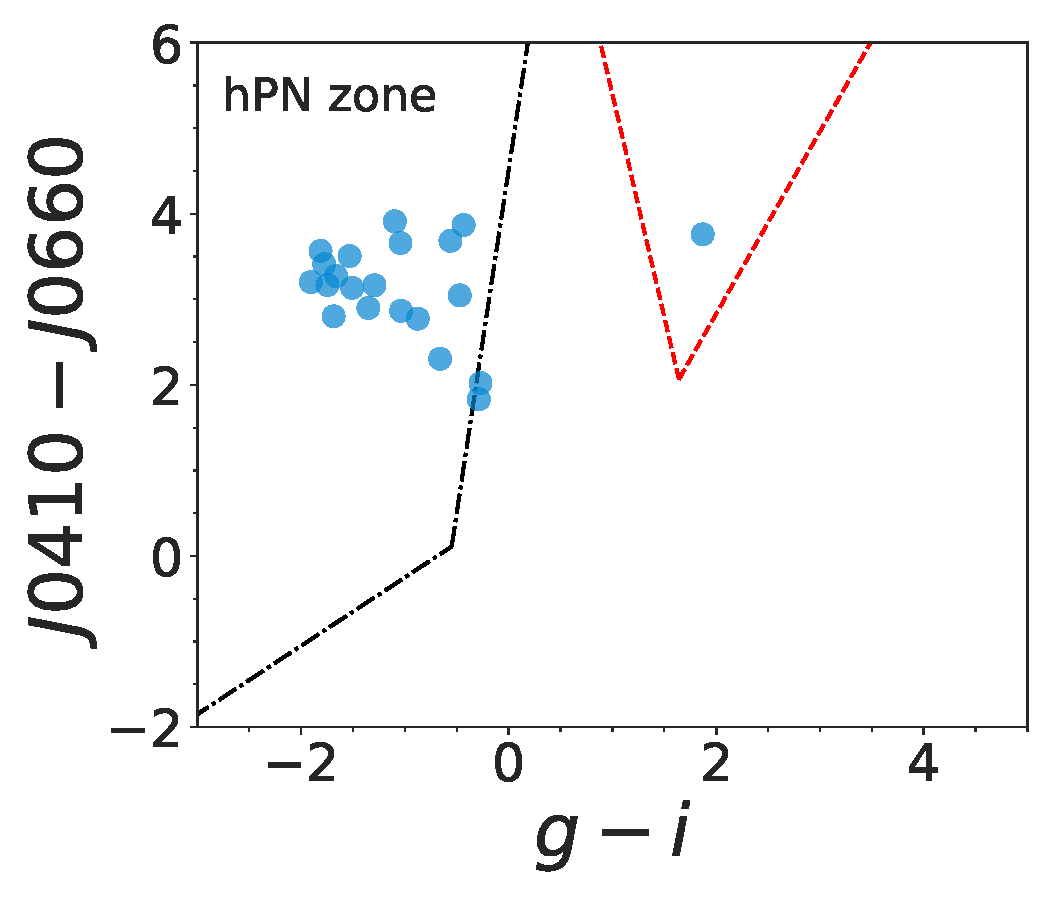
\includegraphics[width=0.5\linewidth, trim=10 10 10 10, clip]{Fig5-IDR2-SPLUS-gi.pdf} \\
%\raiselabel{(\textit{c})} & \raiselabel{(\textit{d})}
  
  \end{tabular}
\end{figure*}

\newpage
\begin{table}
\begin{tabular}{ccc}
\textbf{Aper} & \textbf{Auto} & \textbf{Petro} \\
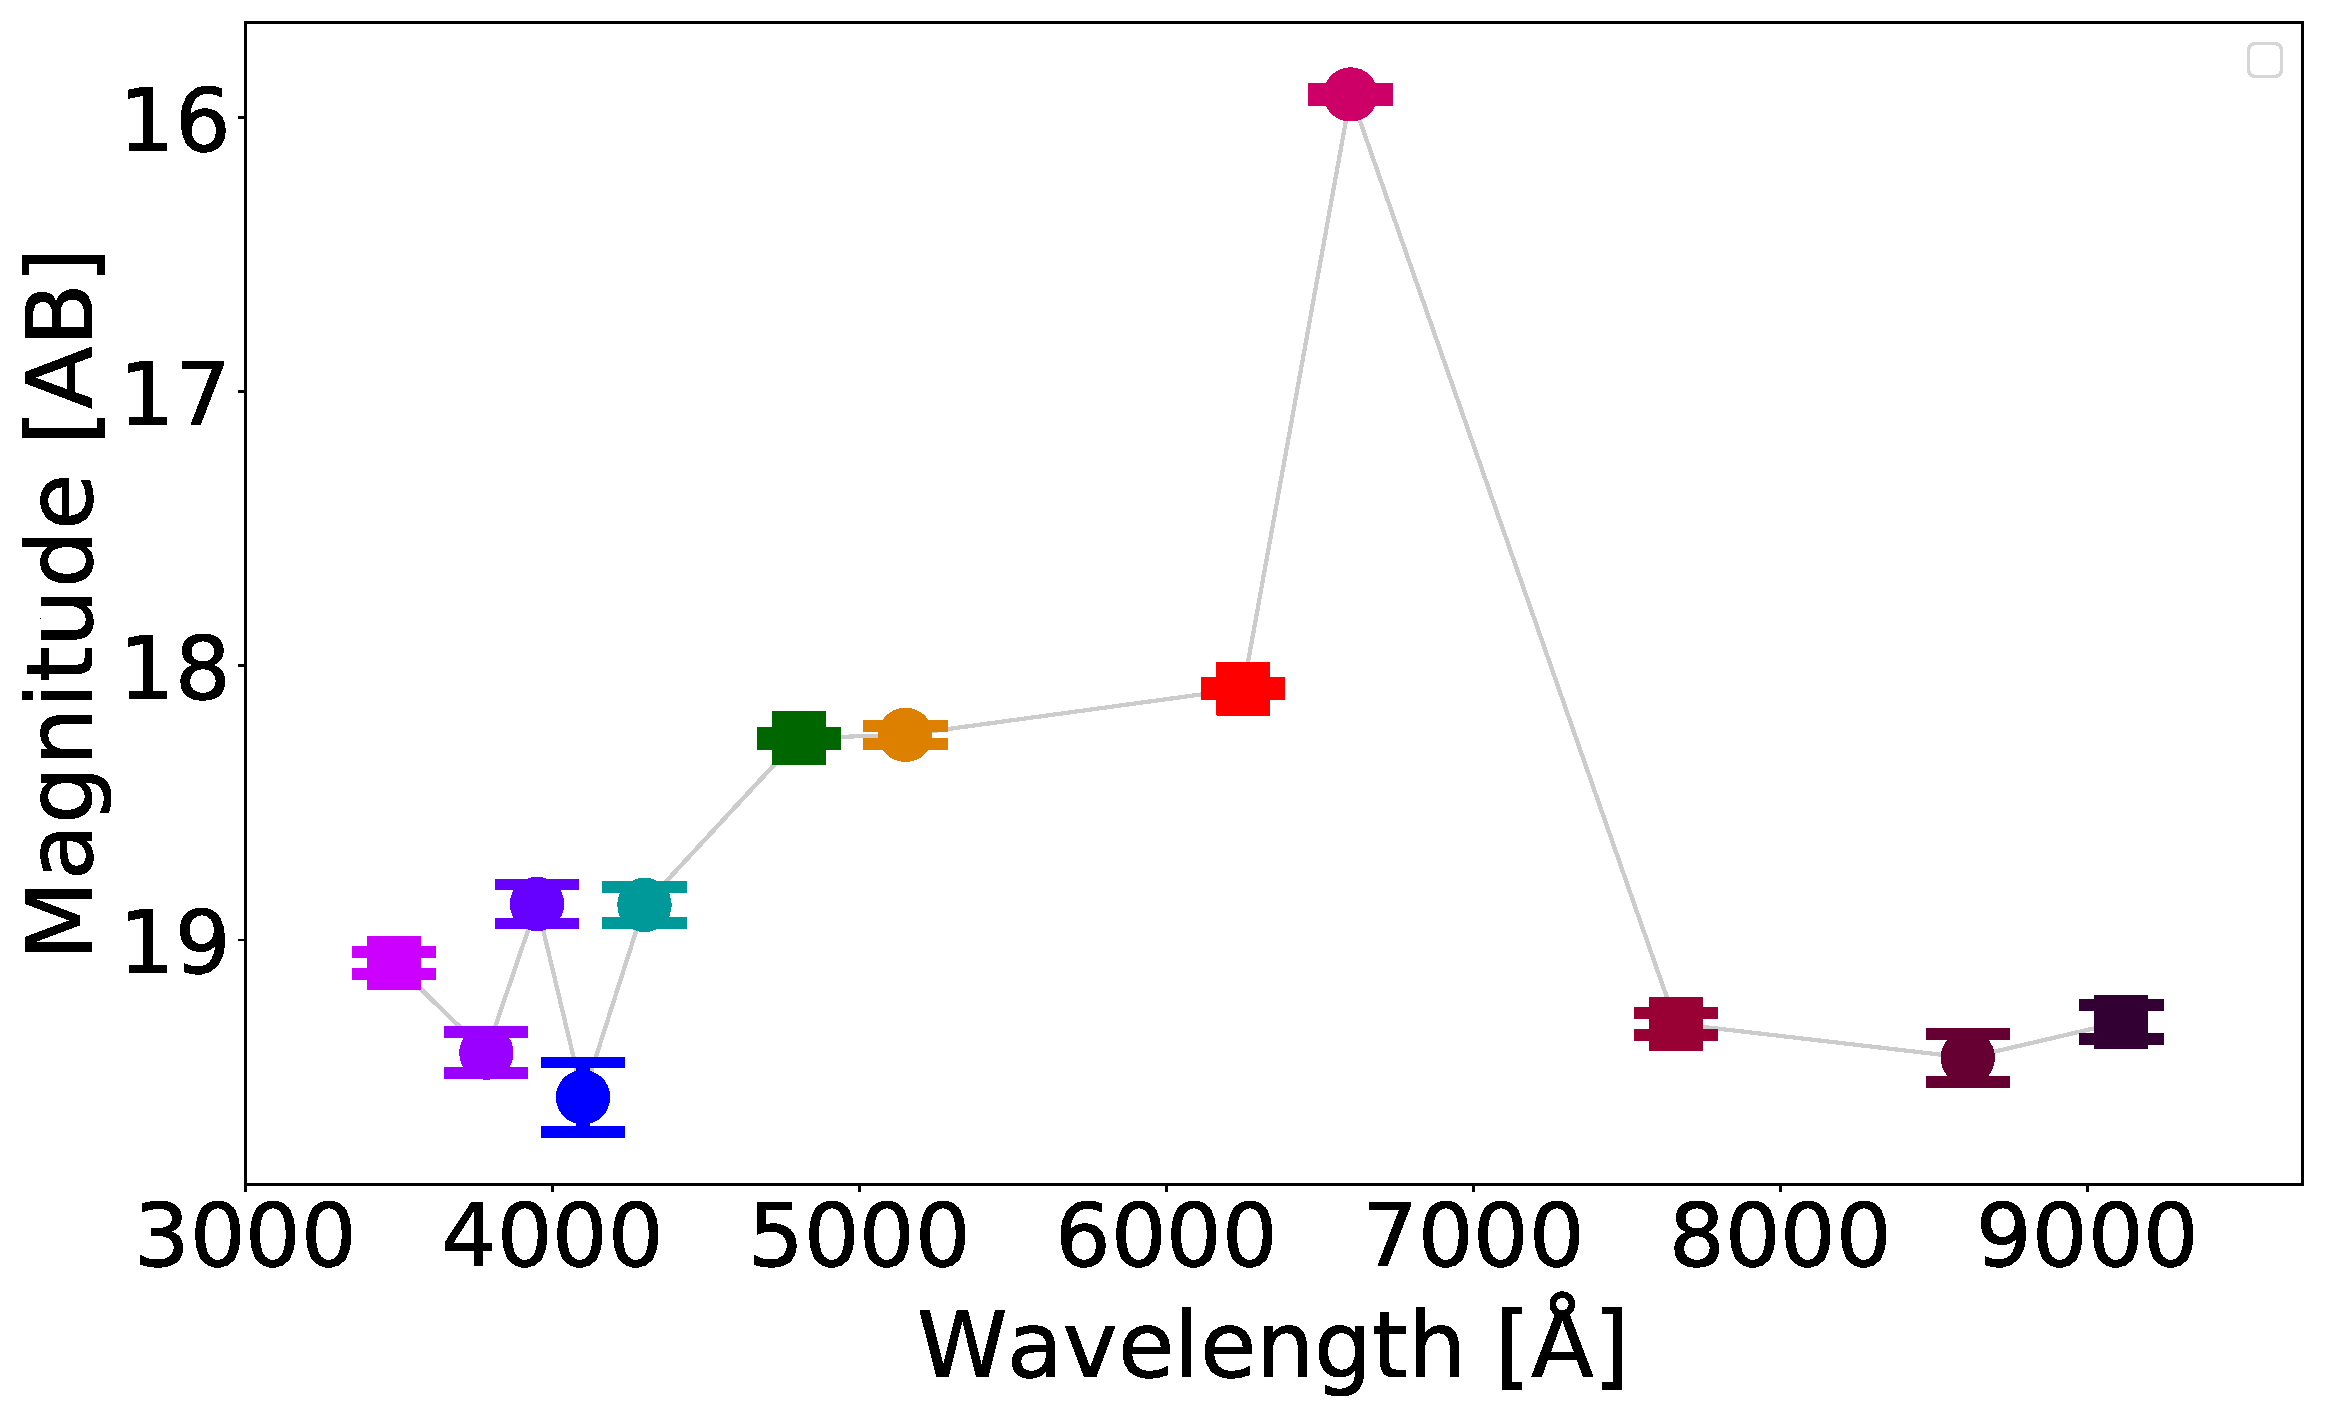
\includegraphics[width=0.3\linewidth, clip]{photopectrum_splus_MC0072-006125_aper.pdf} & 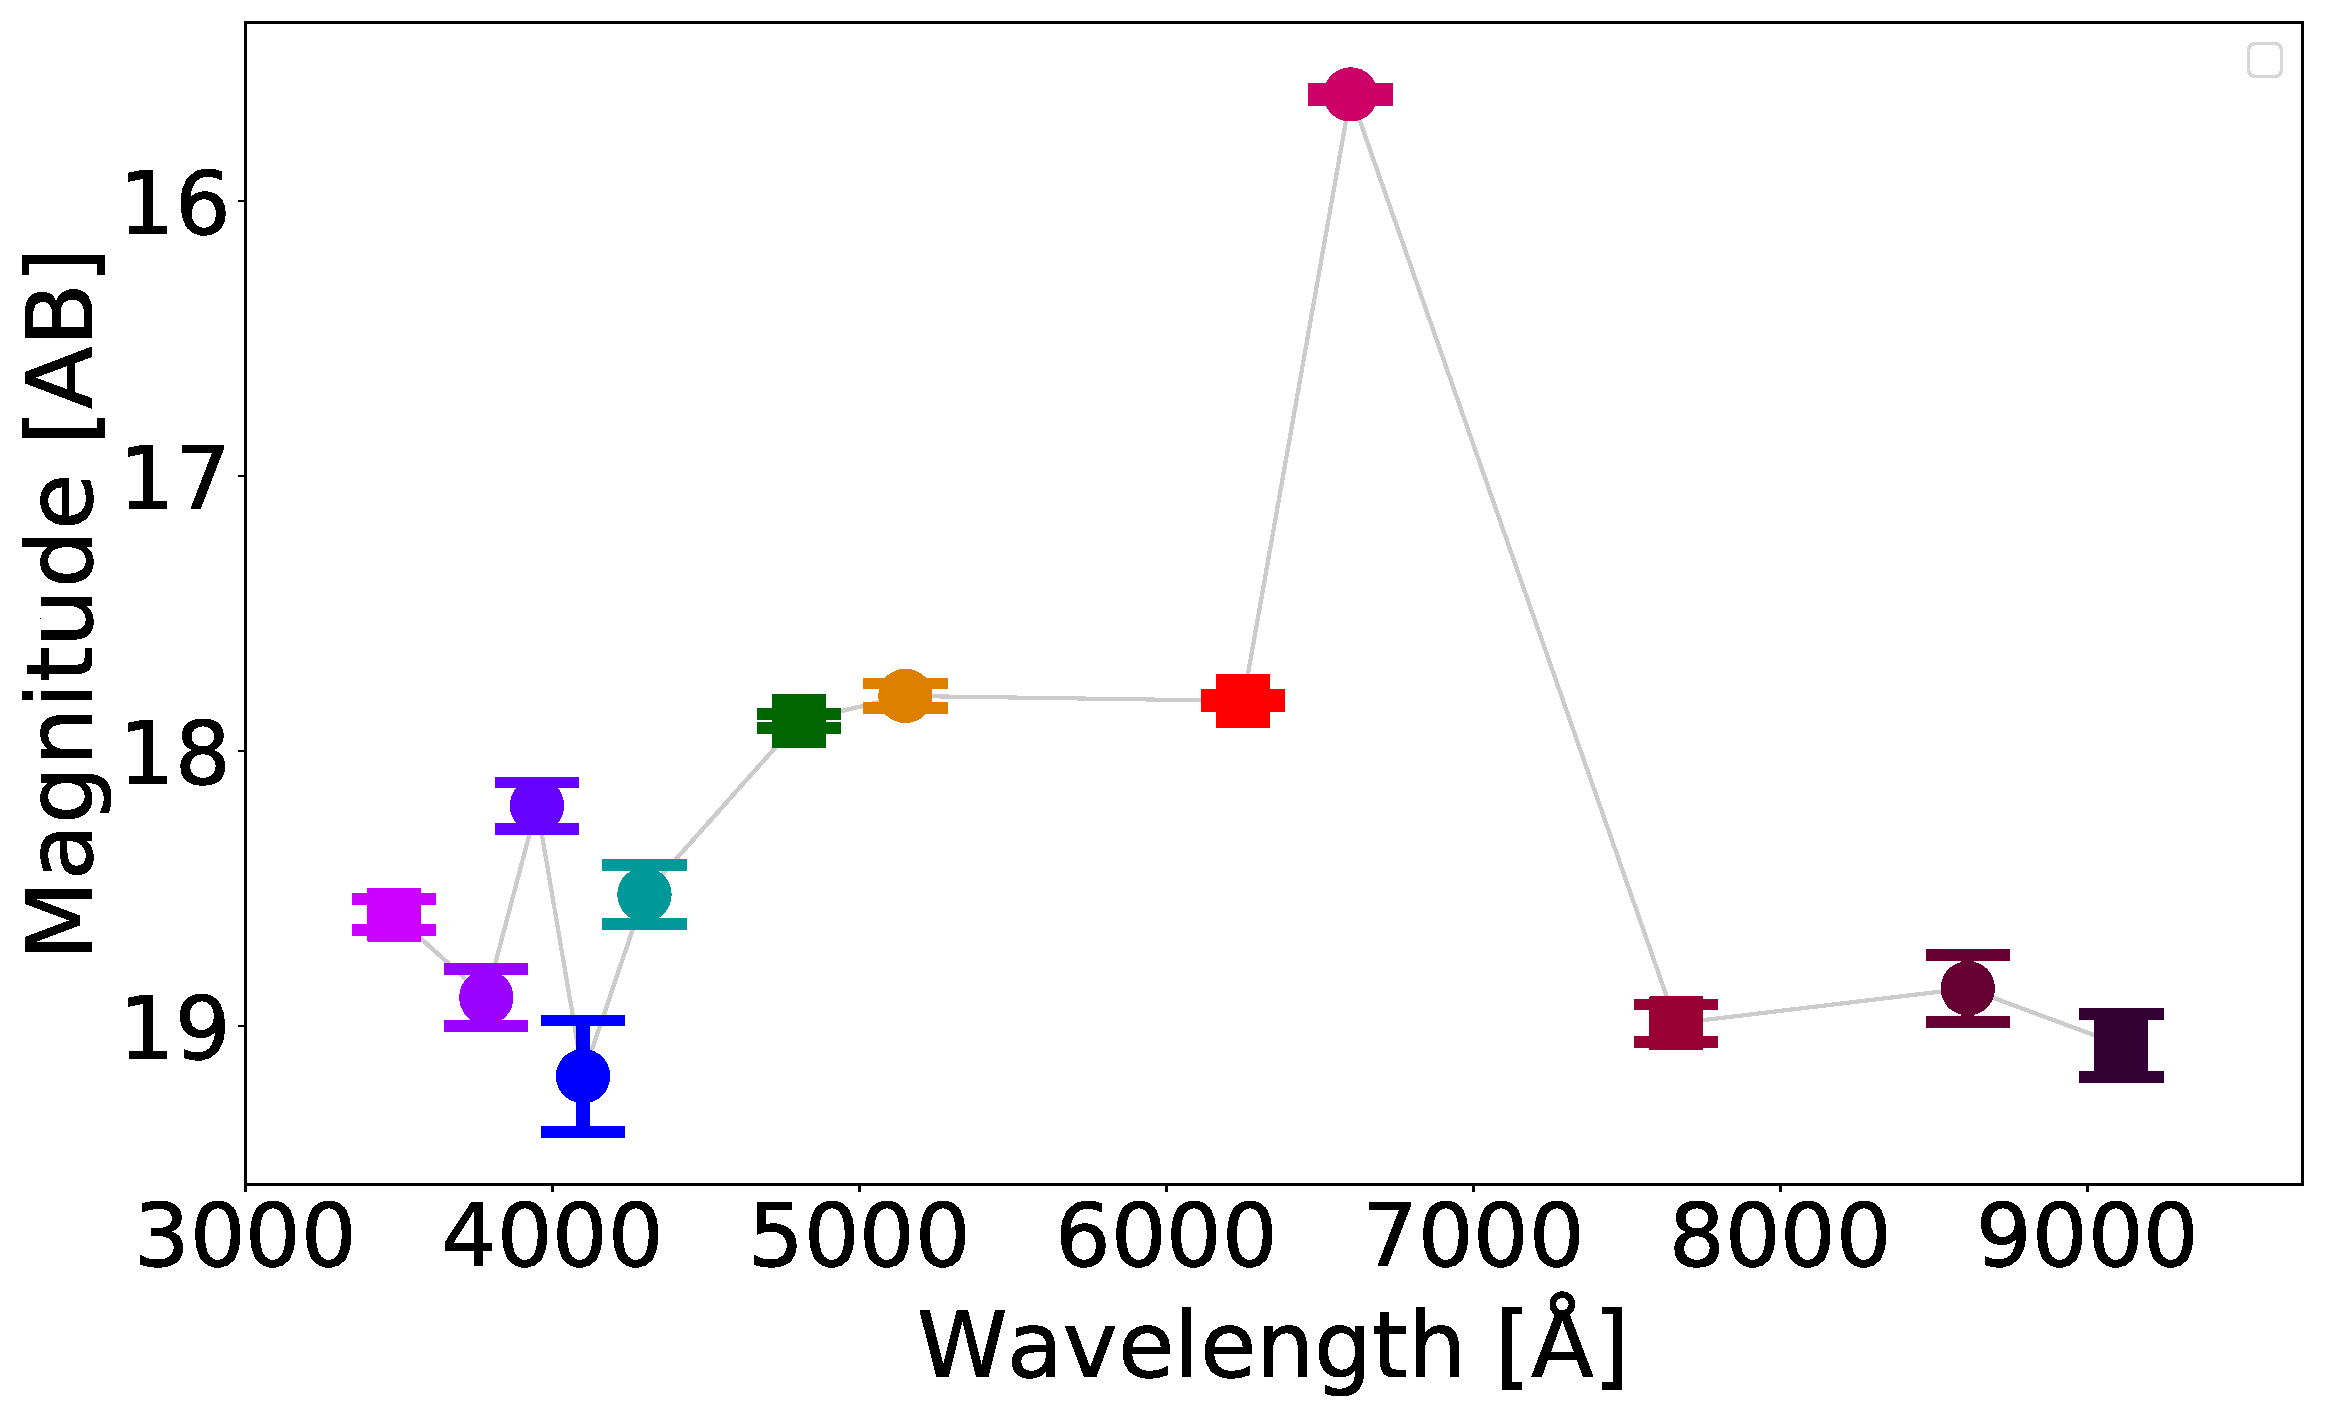
\includegraphics[width=0.3\linewidth, clip]{photopectrum_splus_MC0072-006125_auto.pdf} & 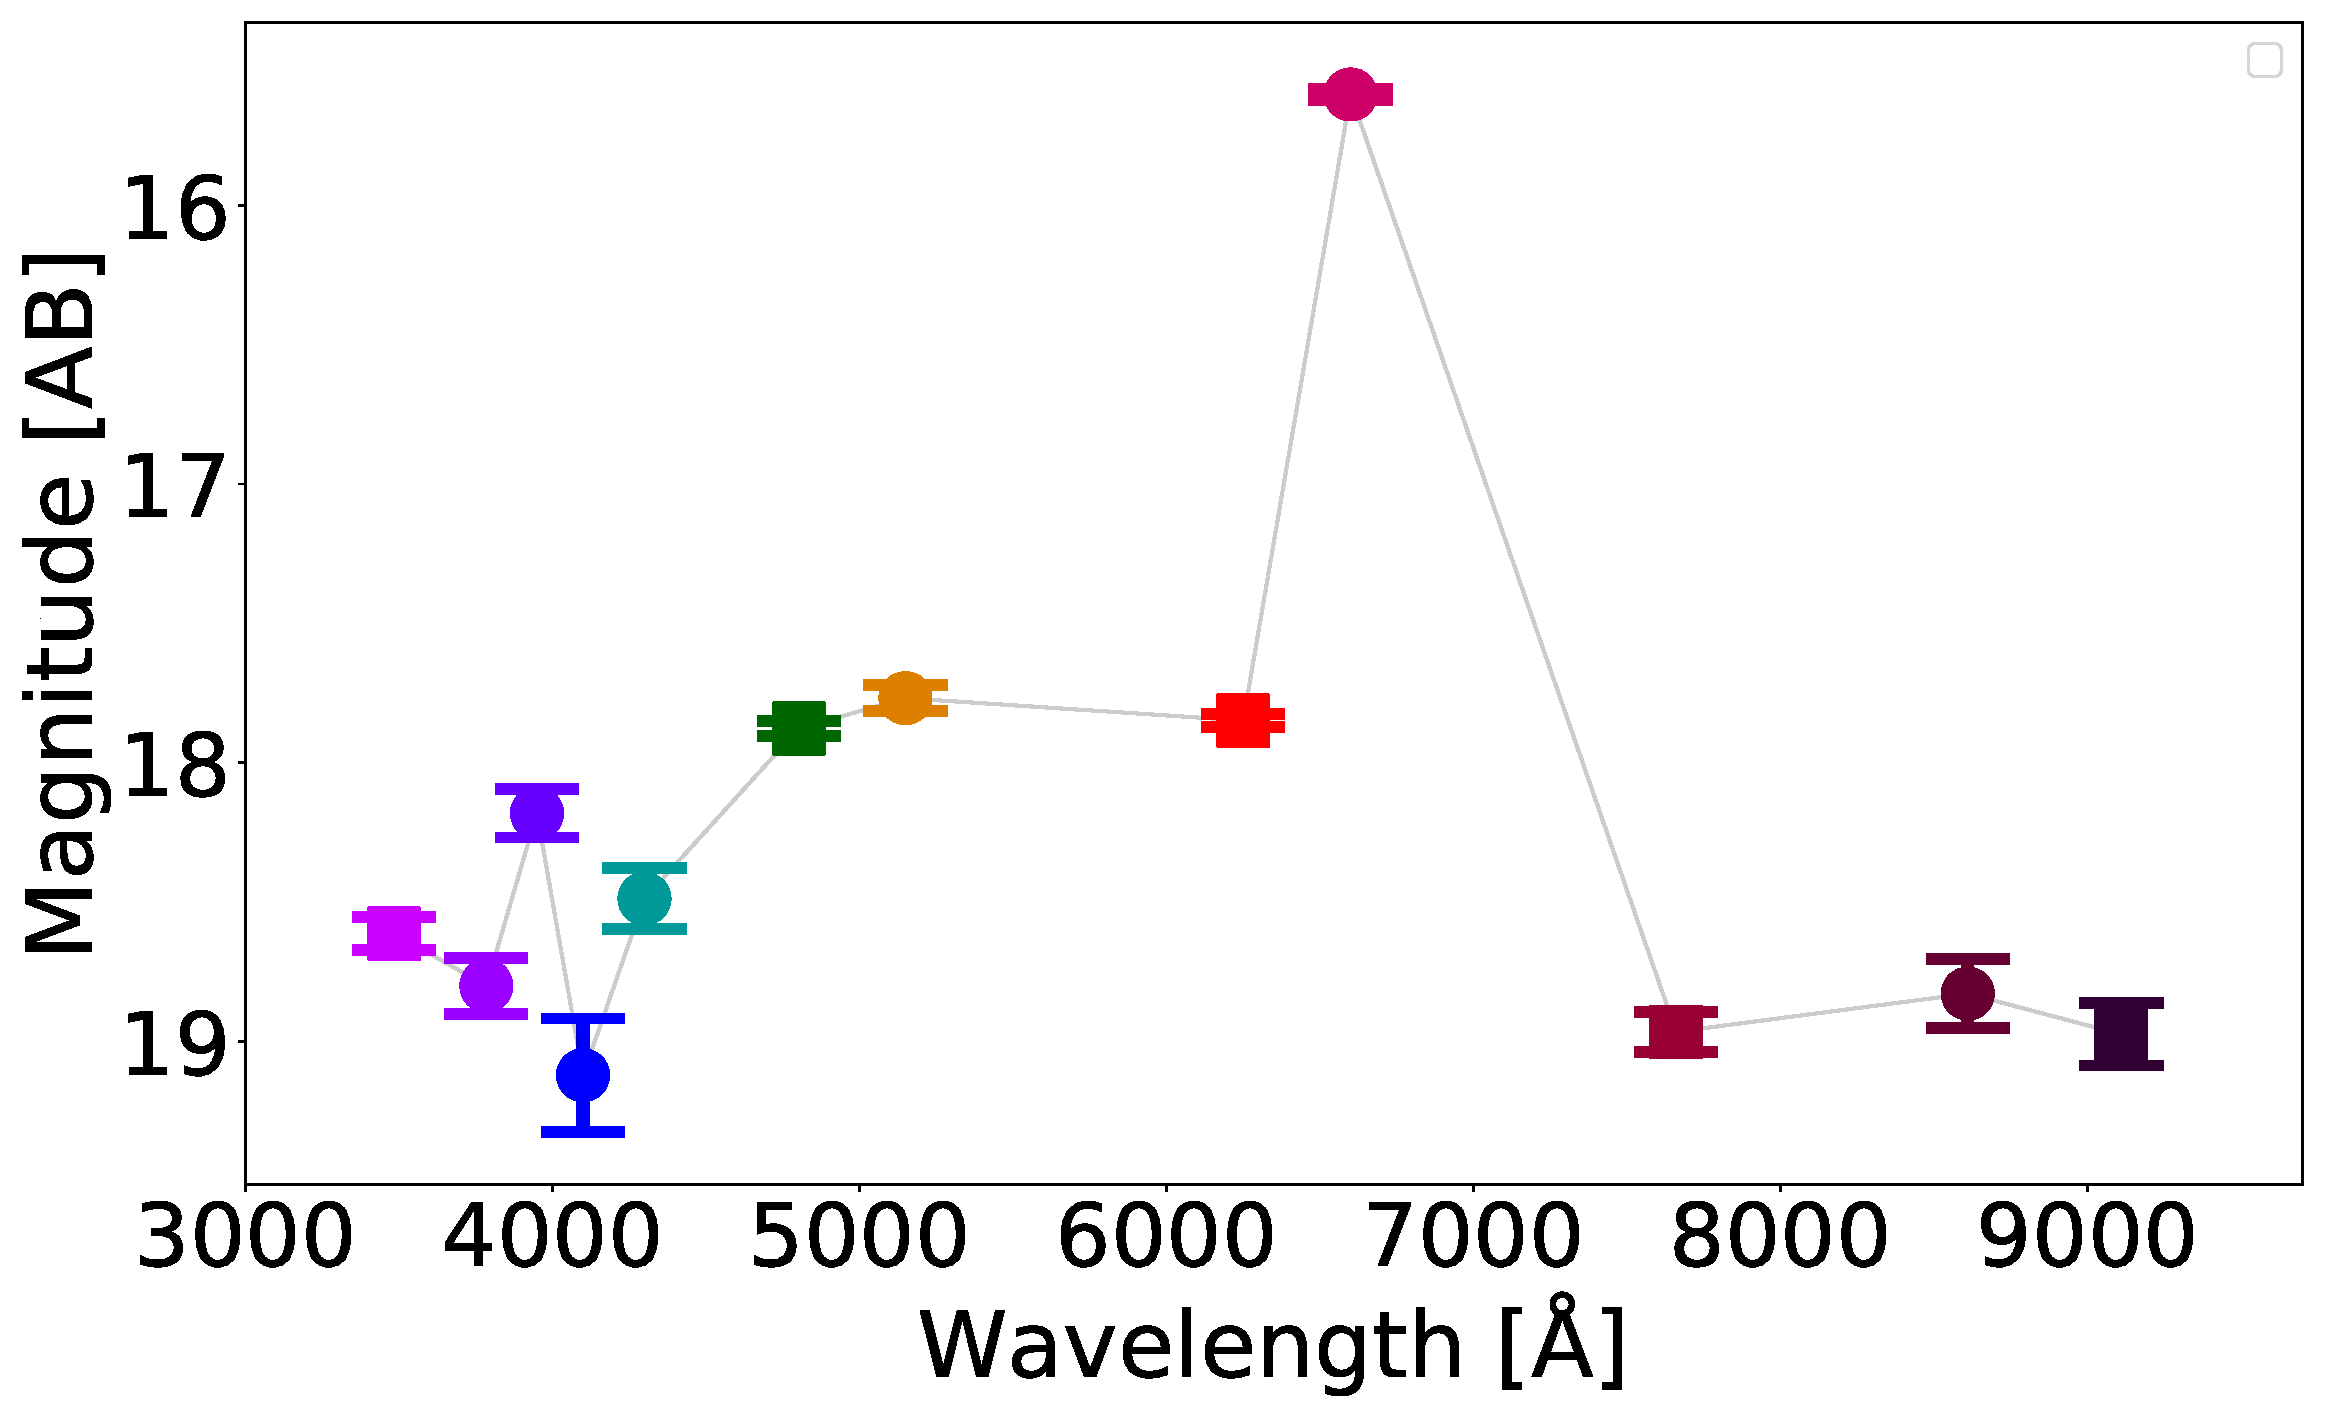
\includegraphics[width=0.3\linewidth, clip]{photopectrum_splus_MC0072-006125_petro.pdf} \\
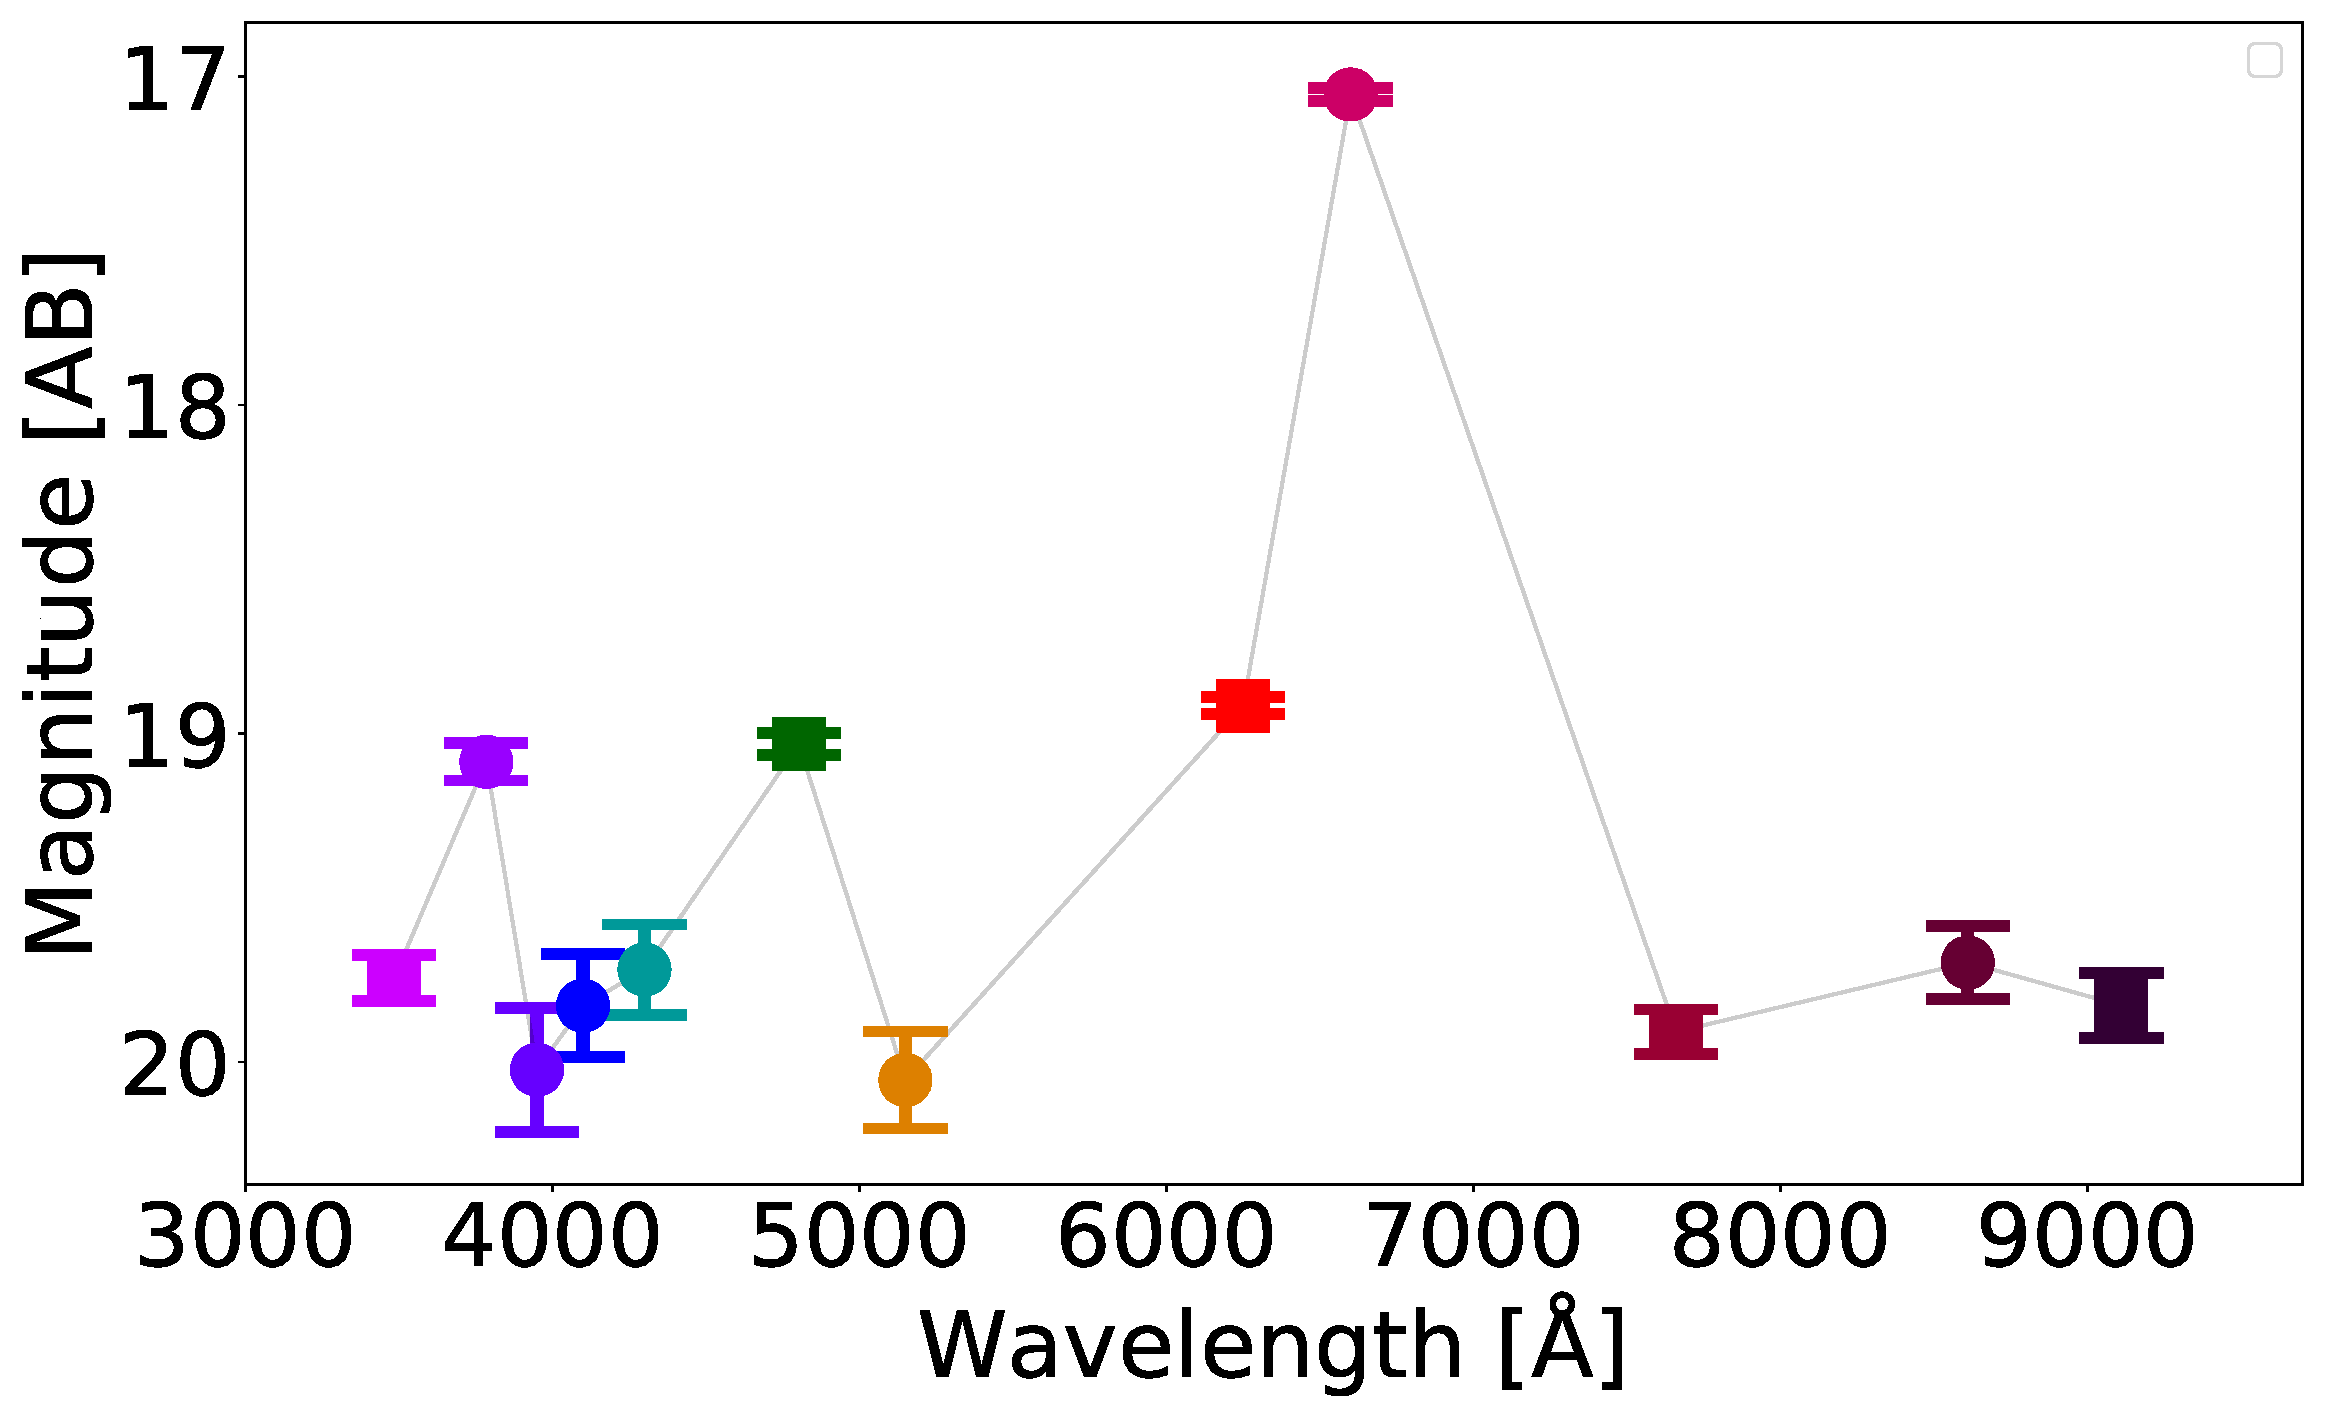
\includegraphics[width=0.3\linewidth, clip]{photopectrum_splus_MC0072-044863_aper.pdf} & 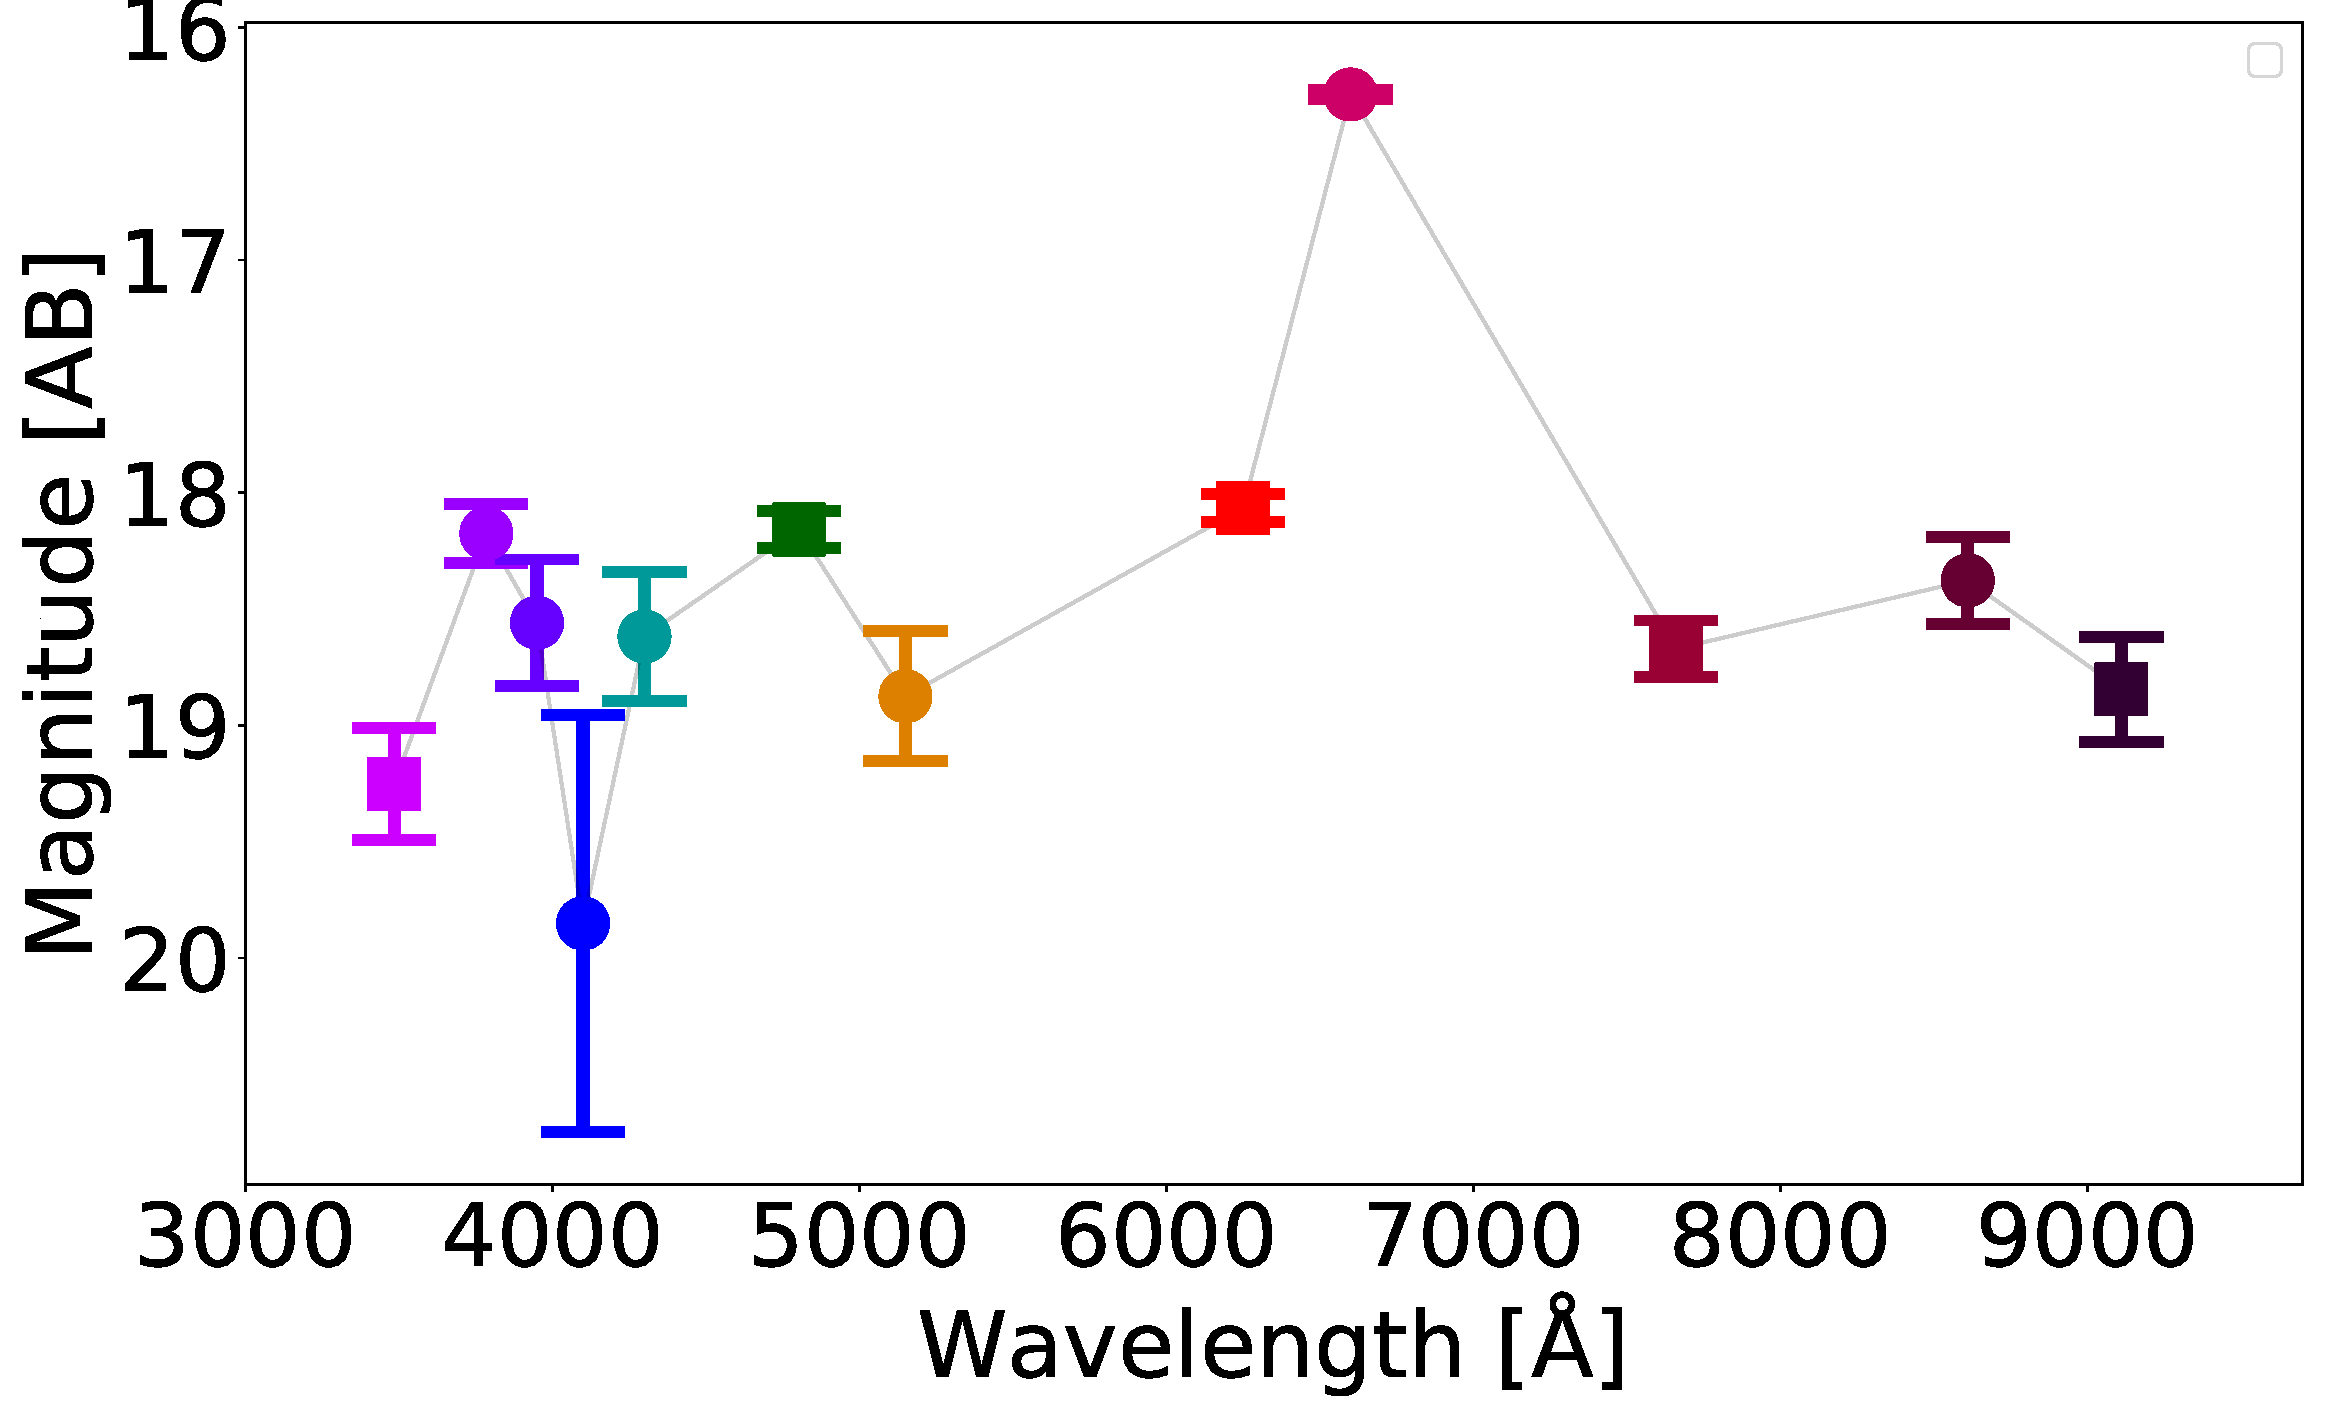
\includegraphics[width=0.3\linewidth, clip]{photopectrum_splus_MC0072-044863_auto.pdf} & 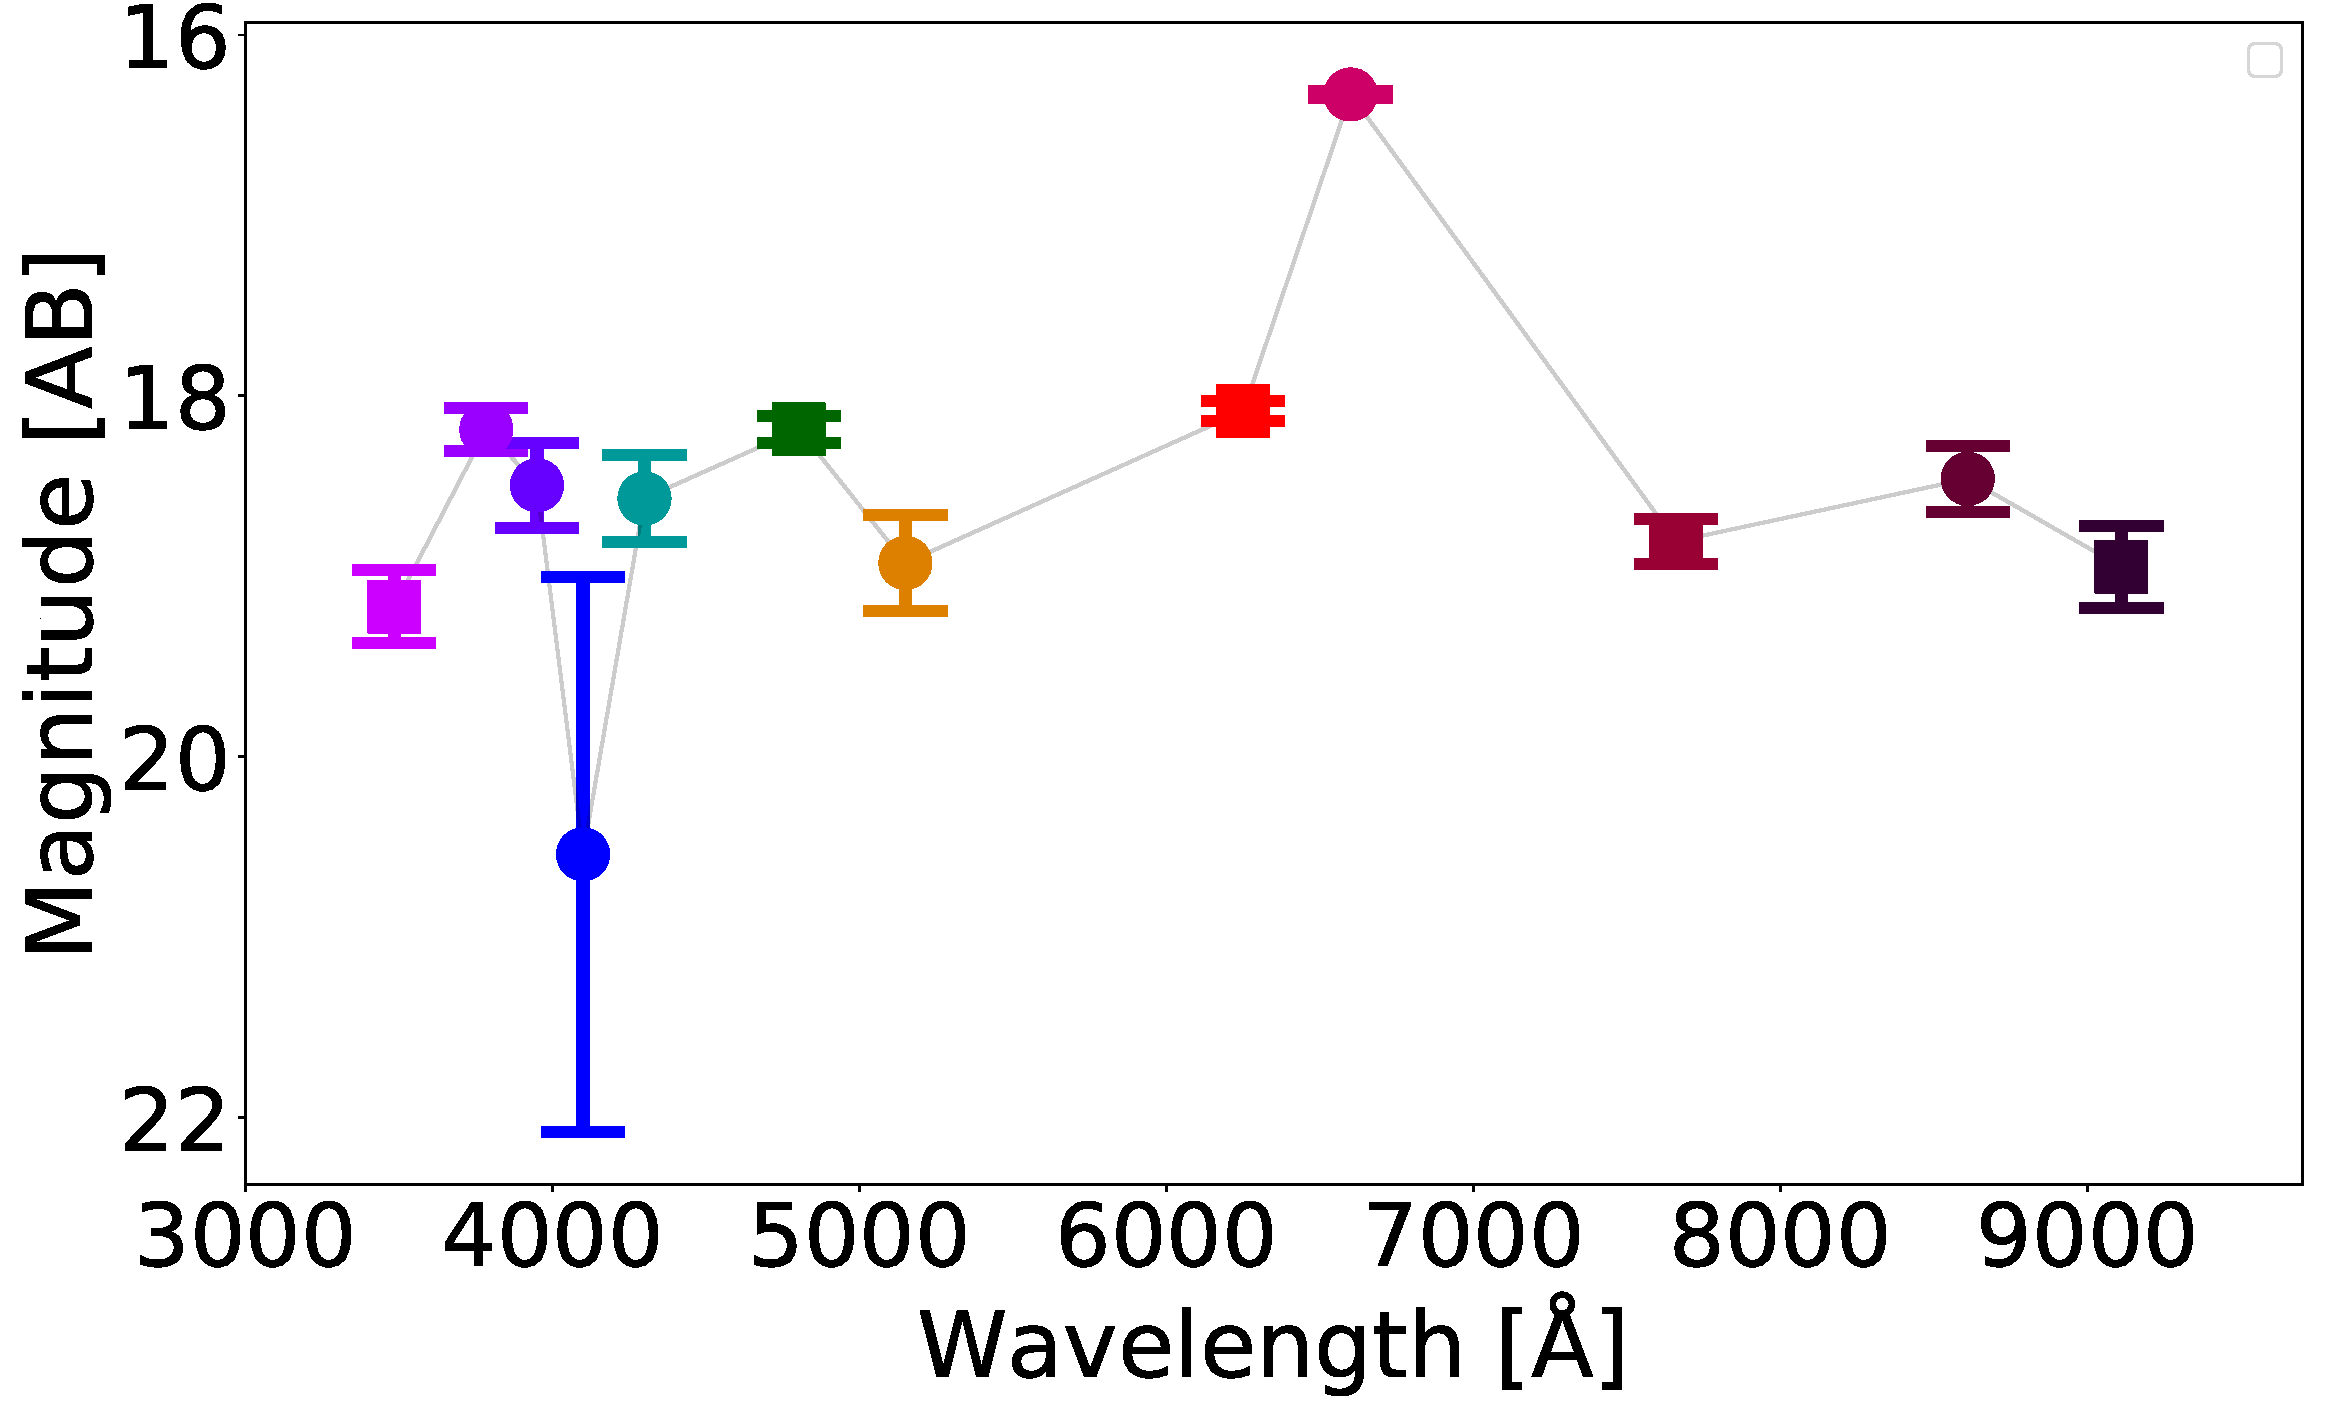
\includegraphics[width=0.3\linewidth, clip]{photopectrum_splus_MC0072-044863_petro.pdf} \\
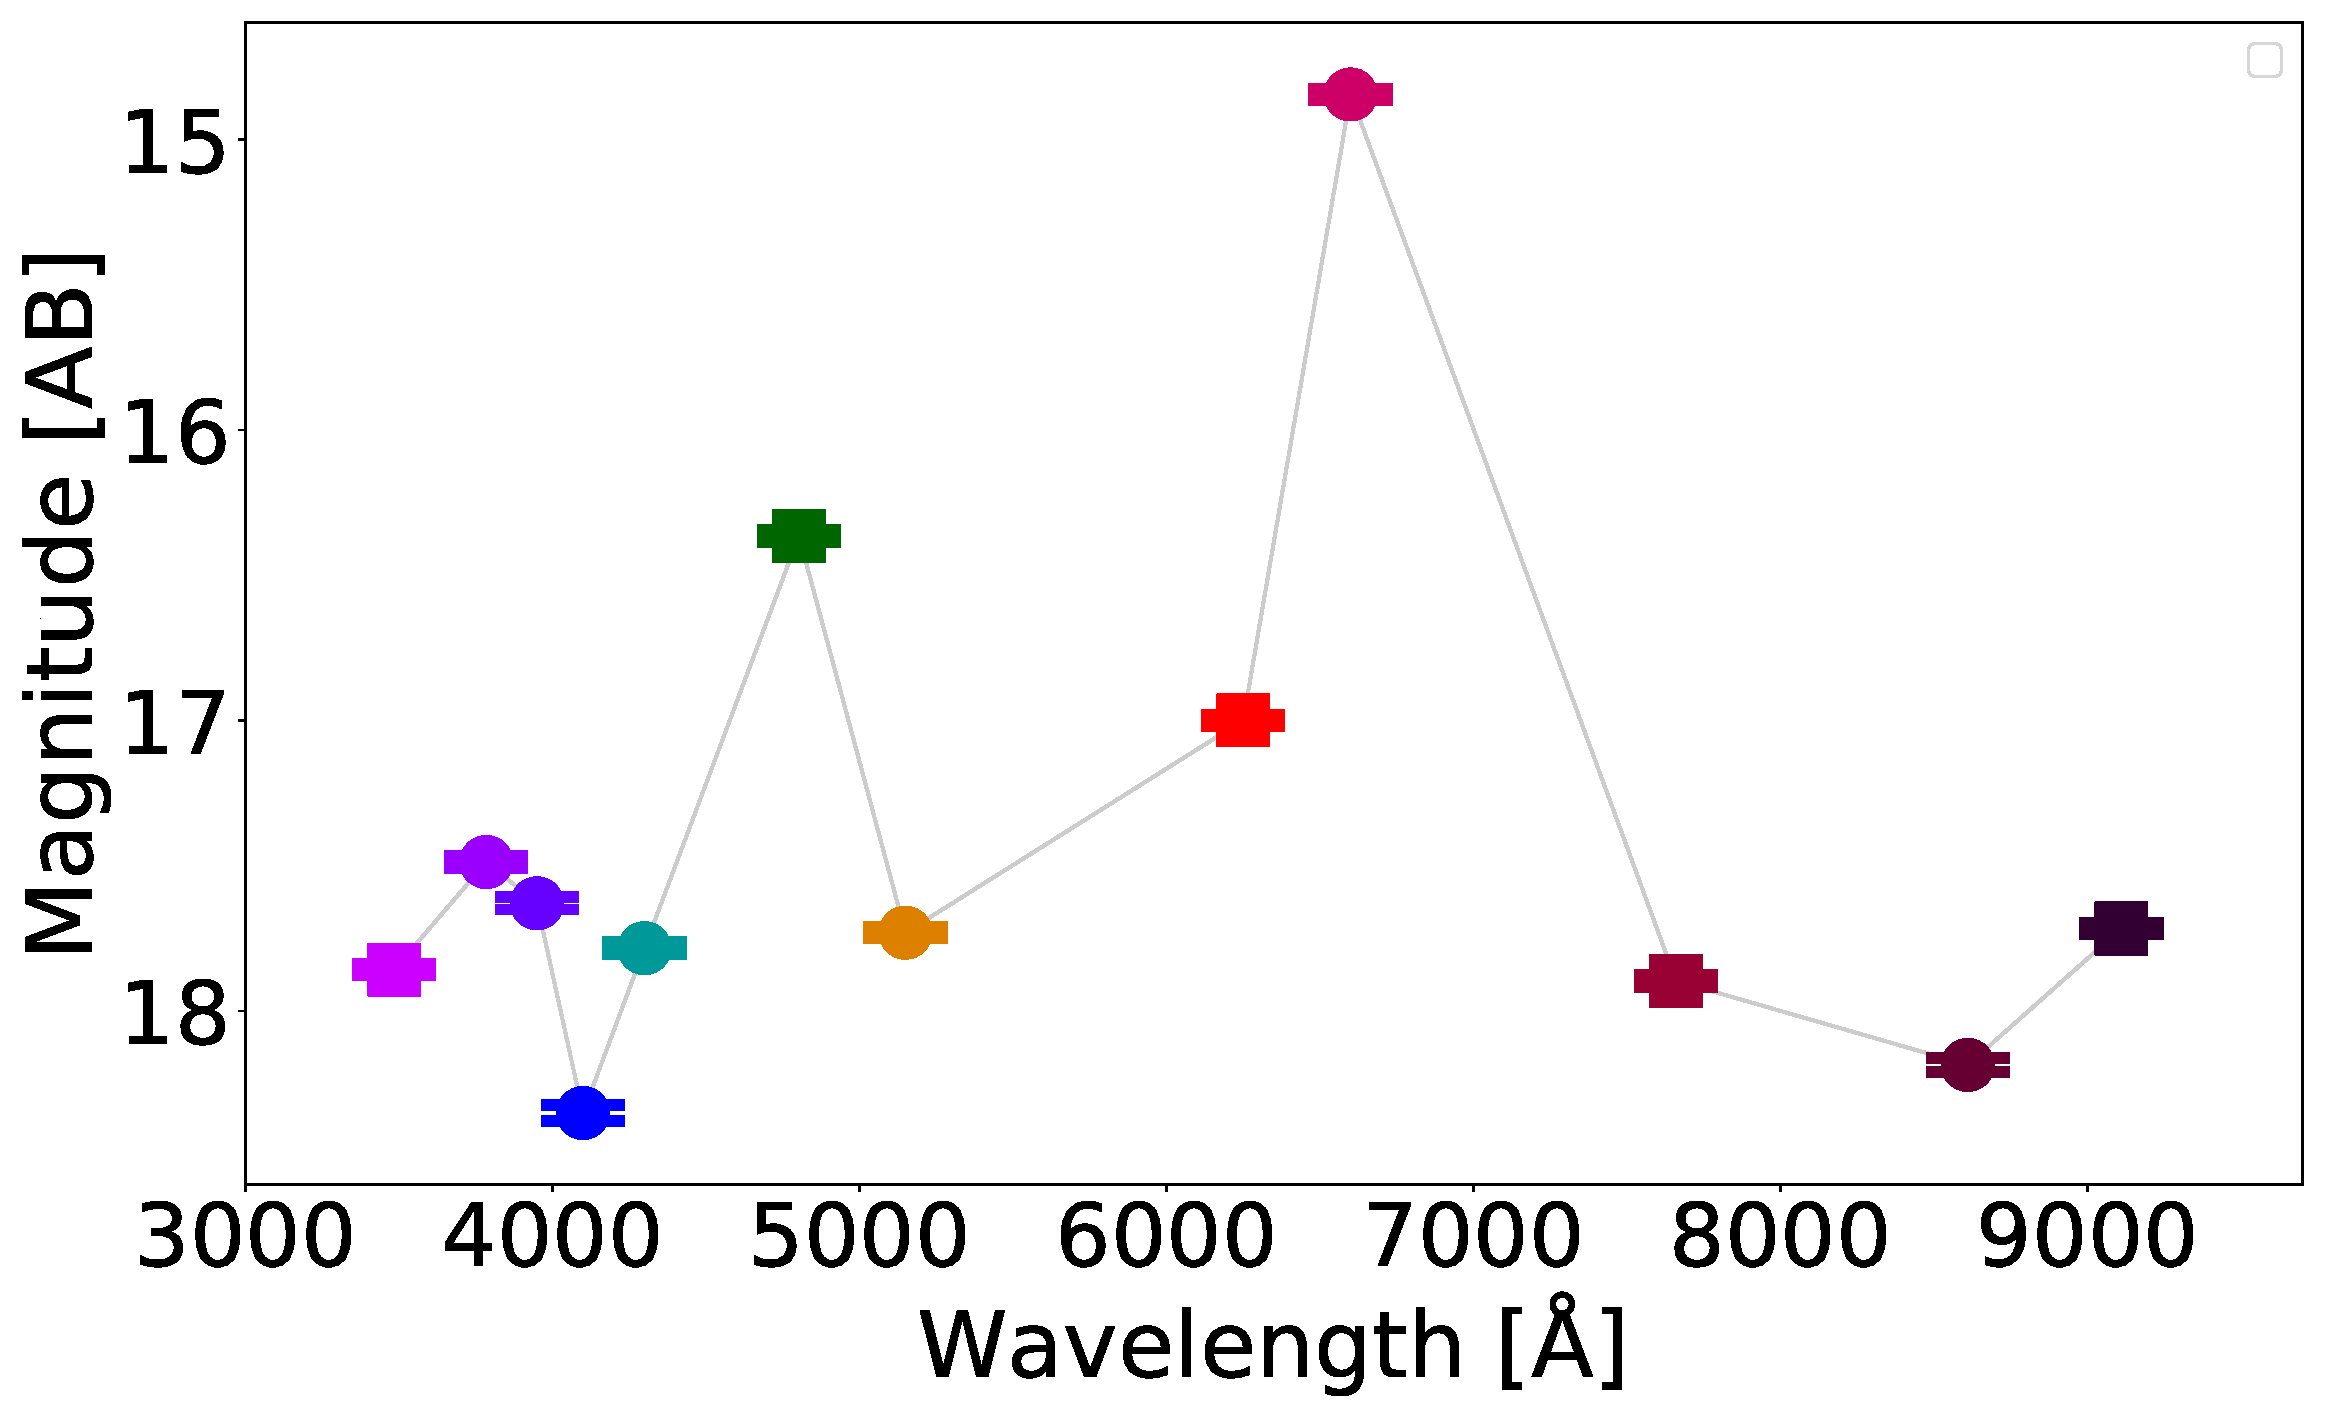
\includegraphics[width=0.3\linewidth, clip]{photopectrum_splus_MC0093-051819_aper.pdf} & 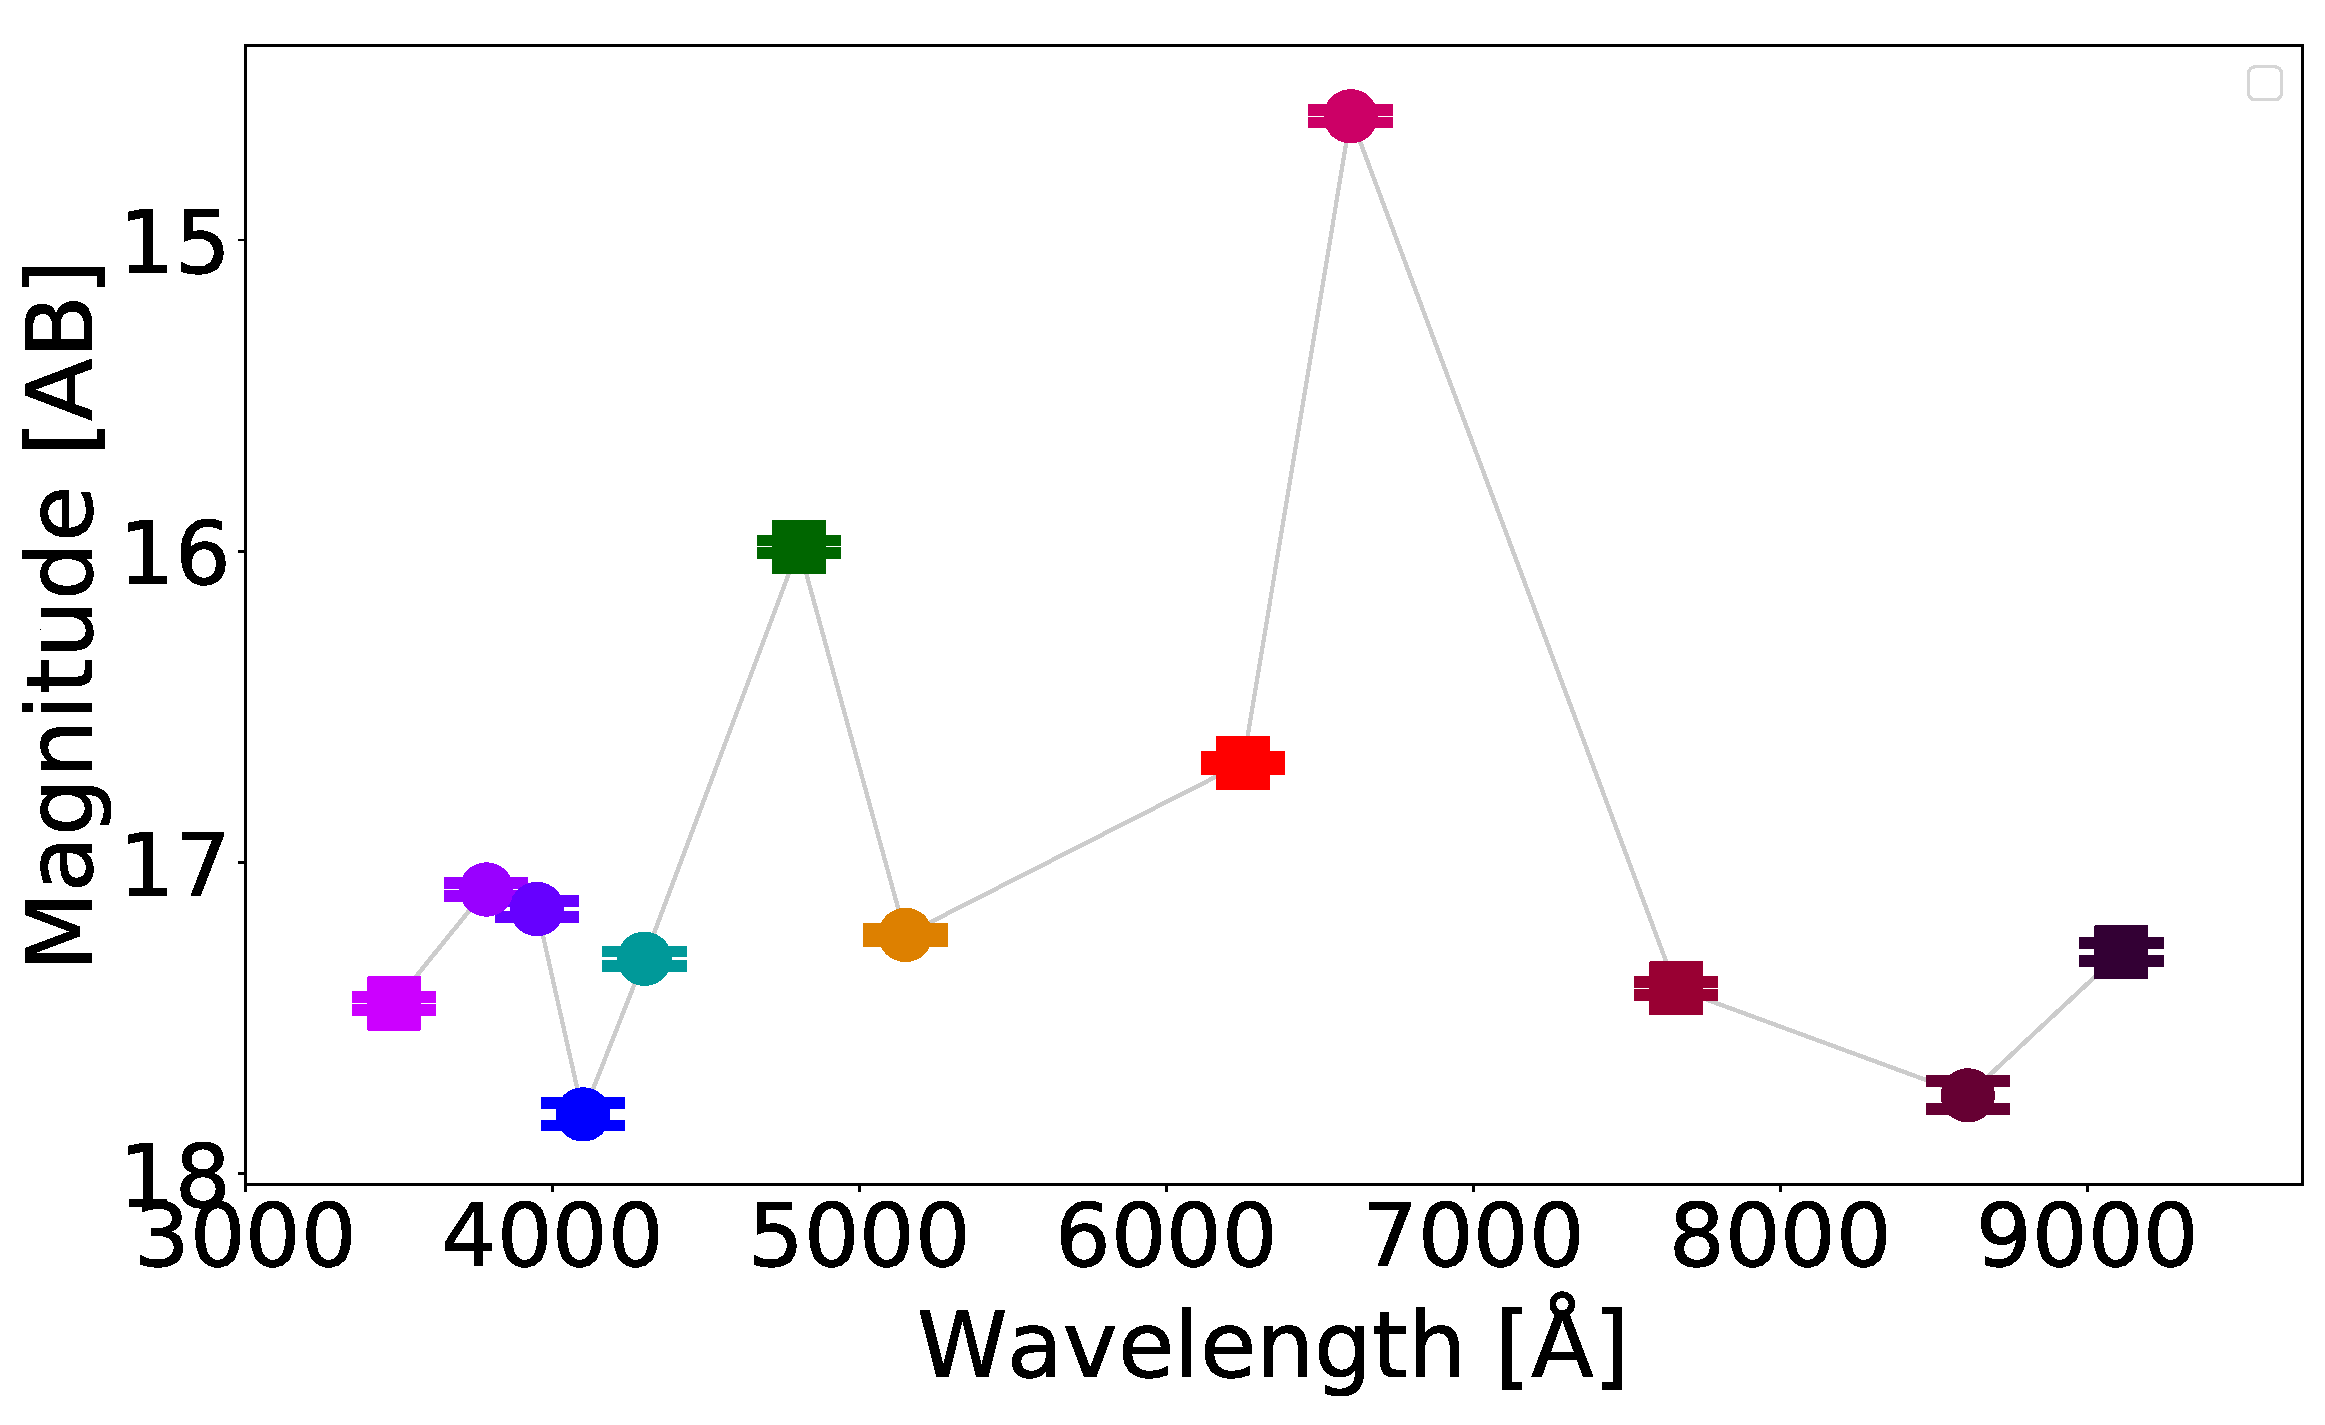
\includegraphics[width=0.3\linewidth, clip]{photopectrum_splus_MC0093-051819_auto.pdf} & 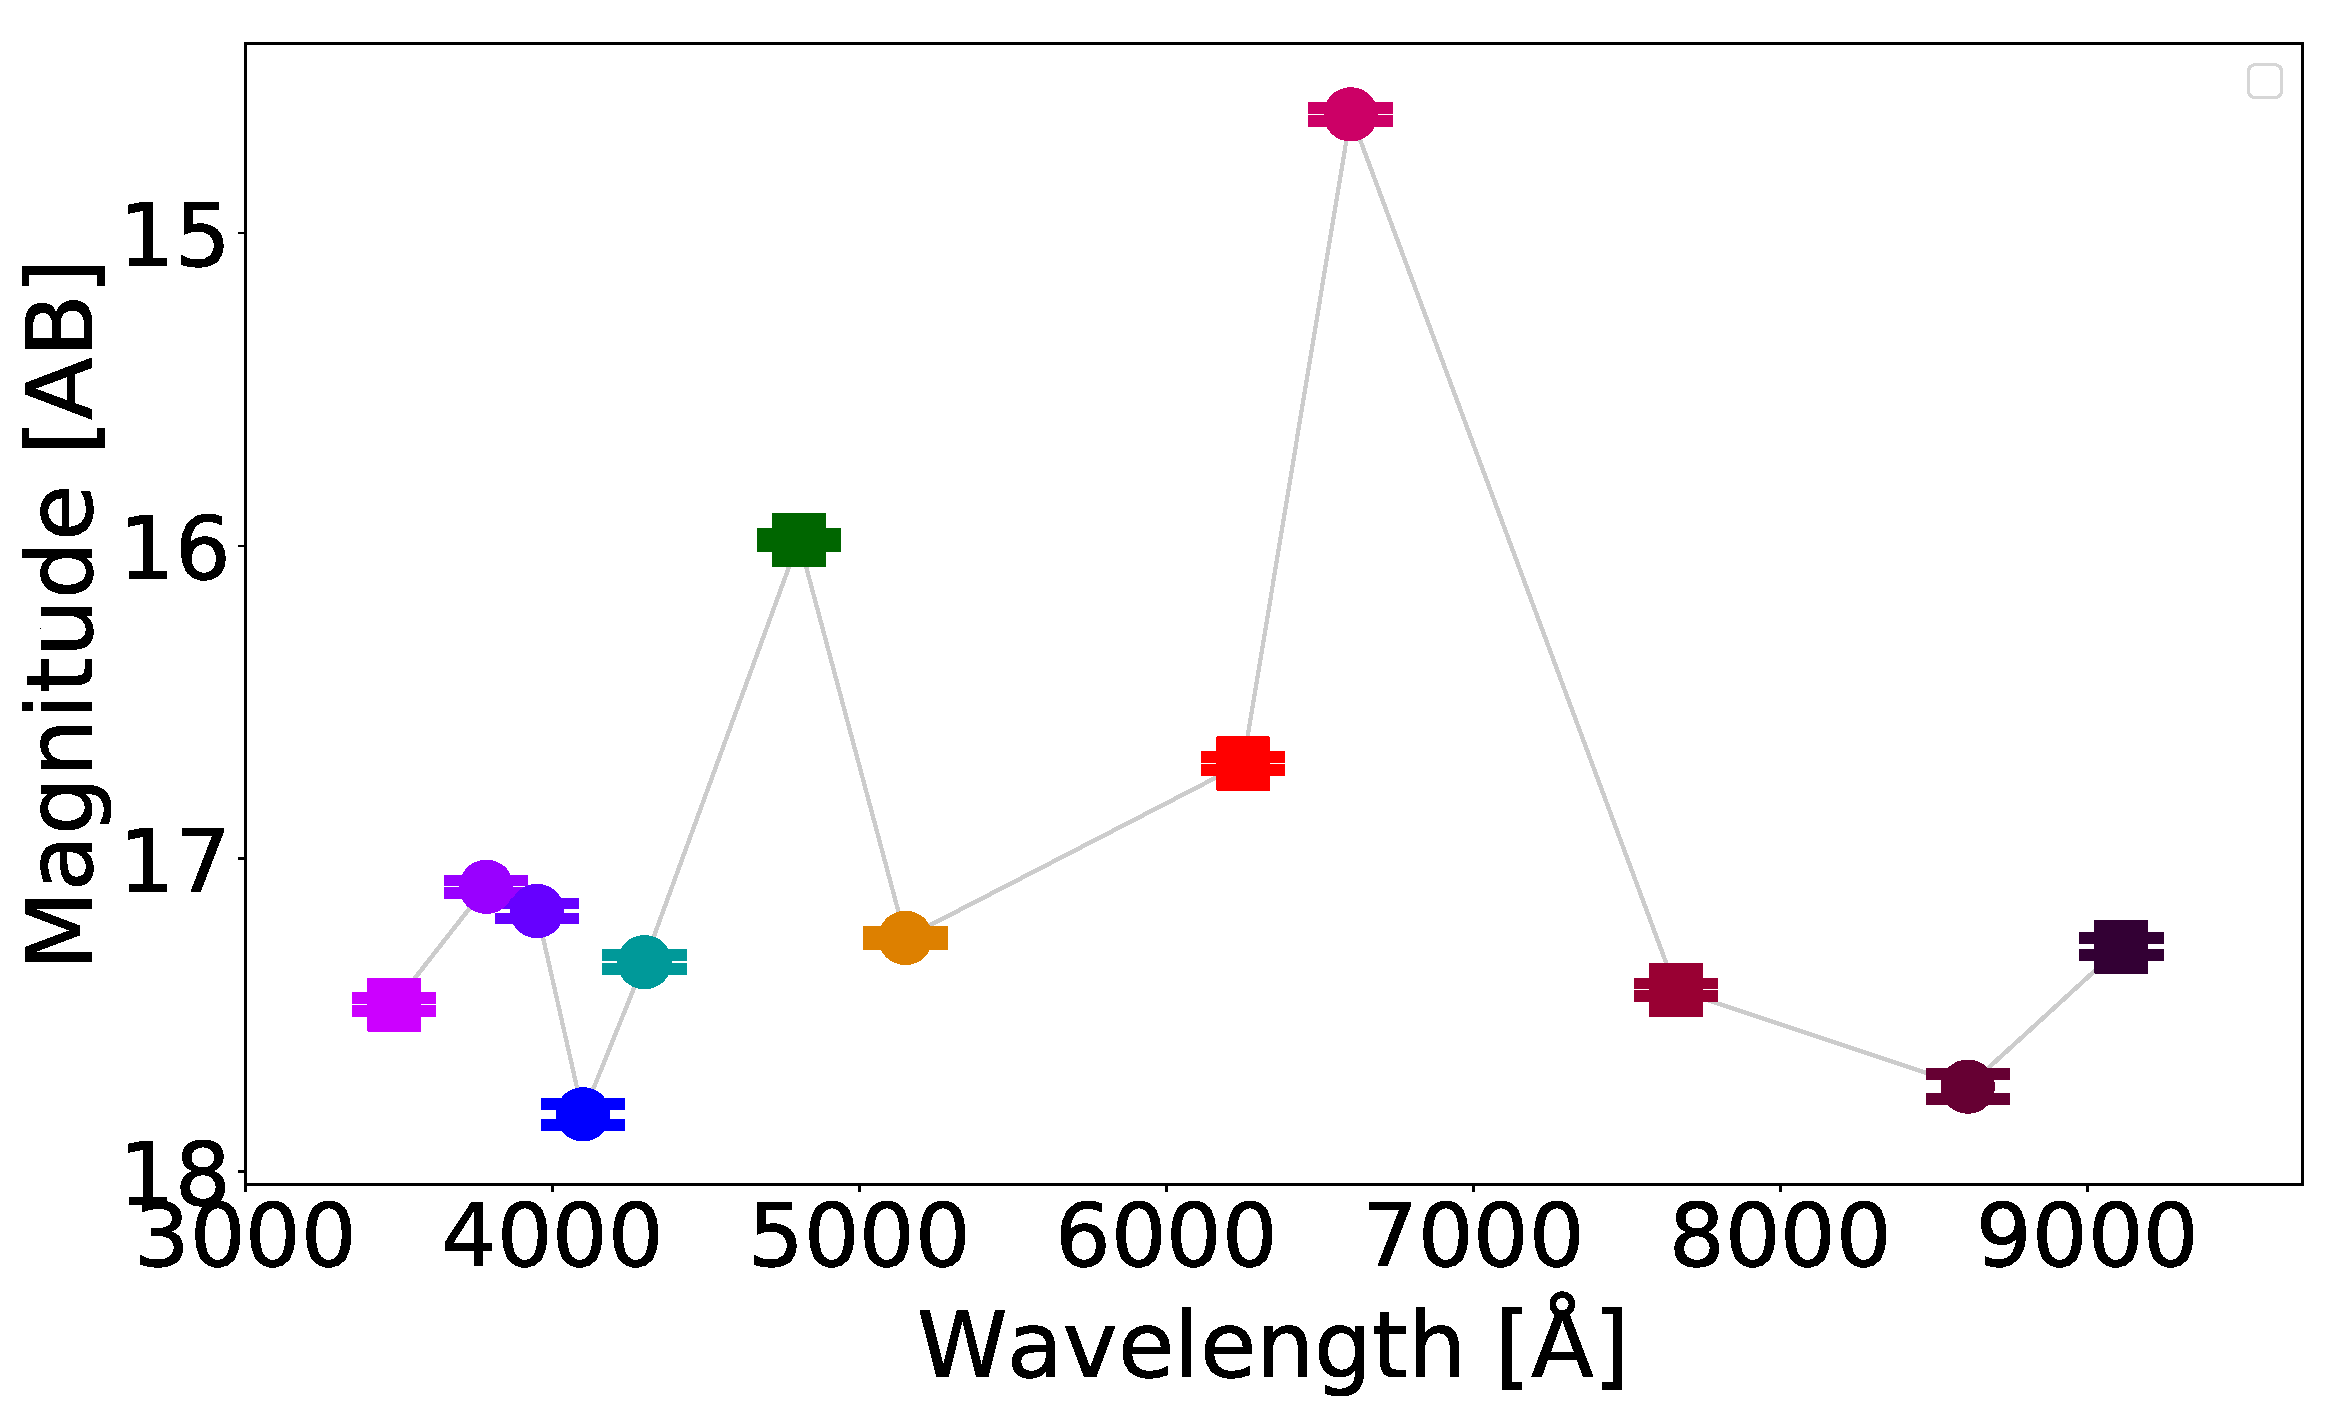
\includegraphics[width=0.3\linewidth, clip]{photopectrum_splus_MC0093-051819_petro.pdf} \\
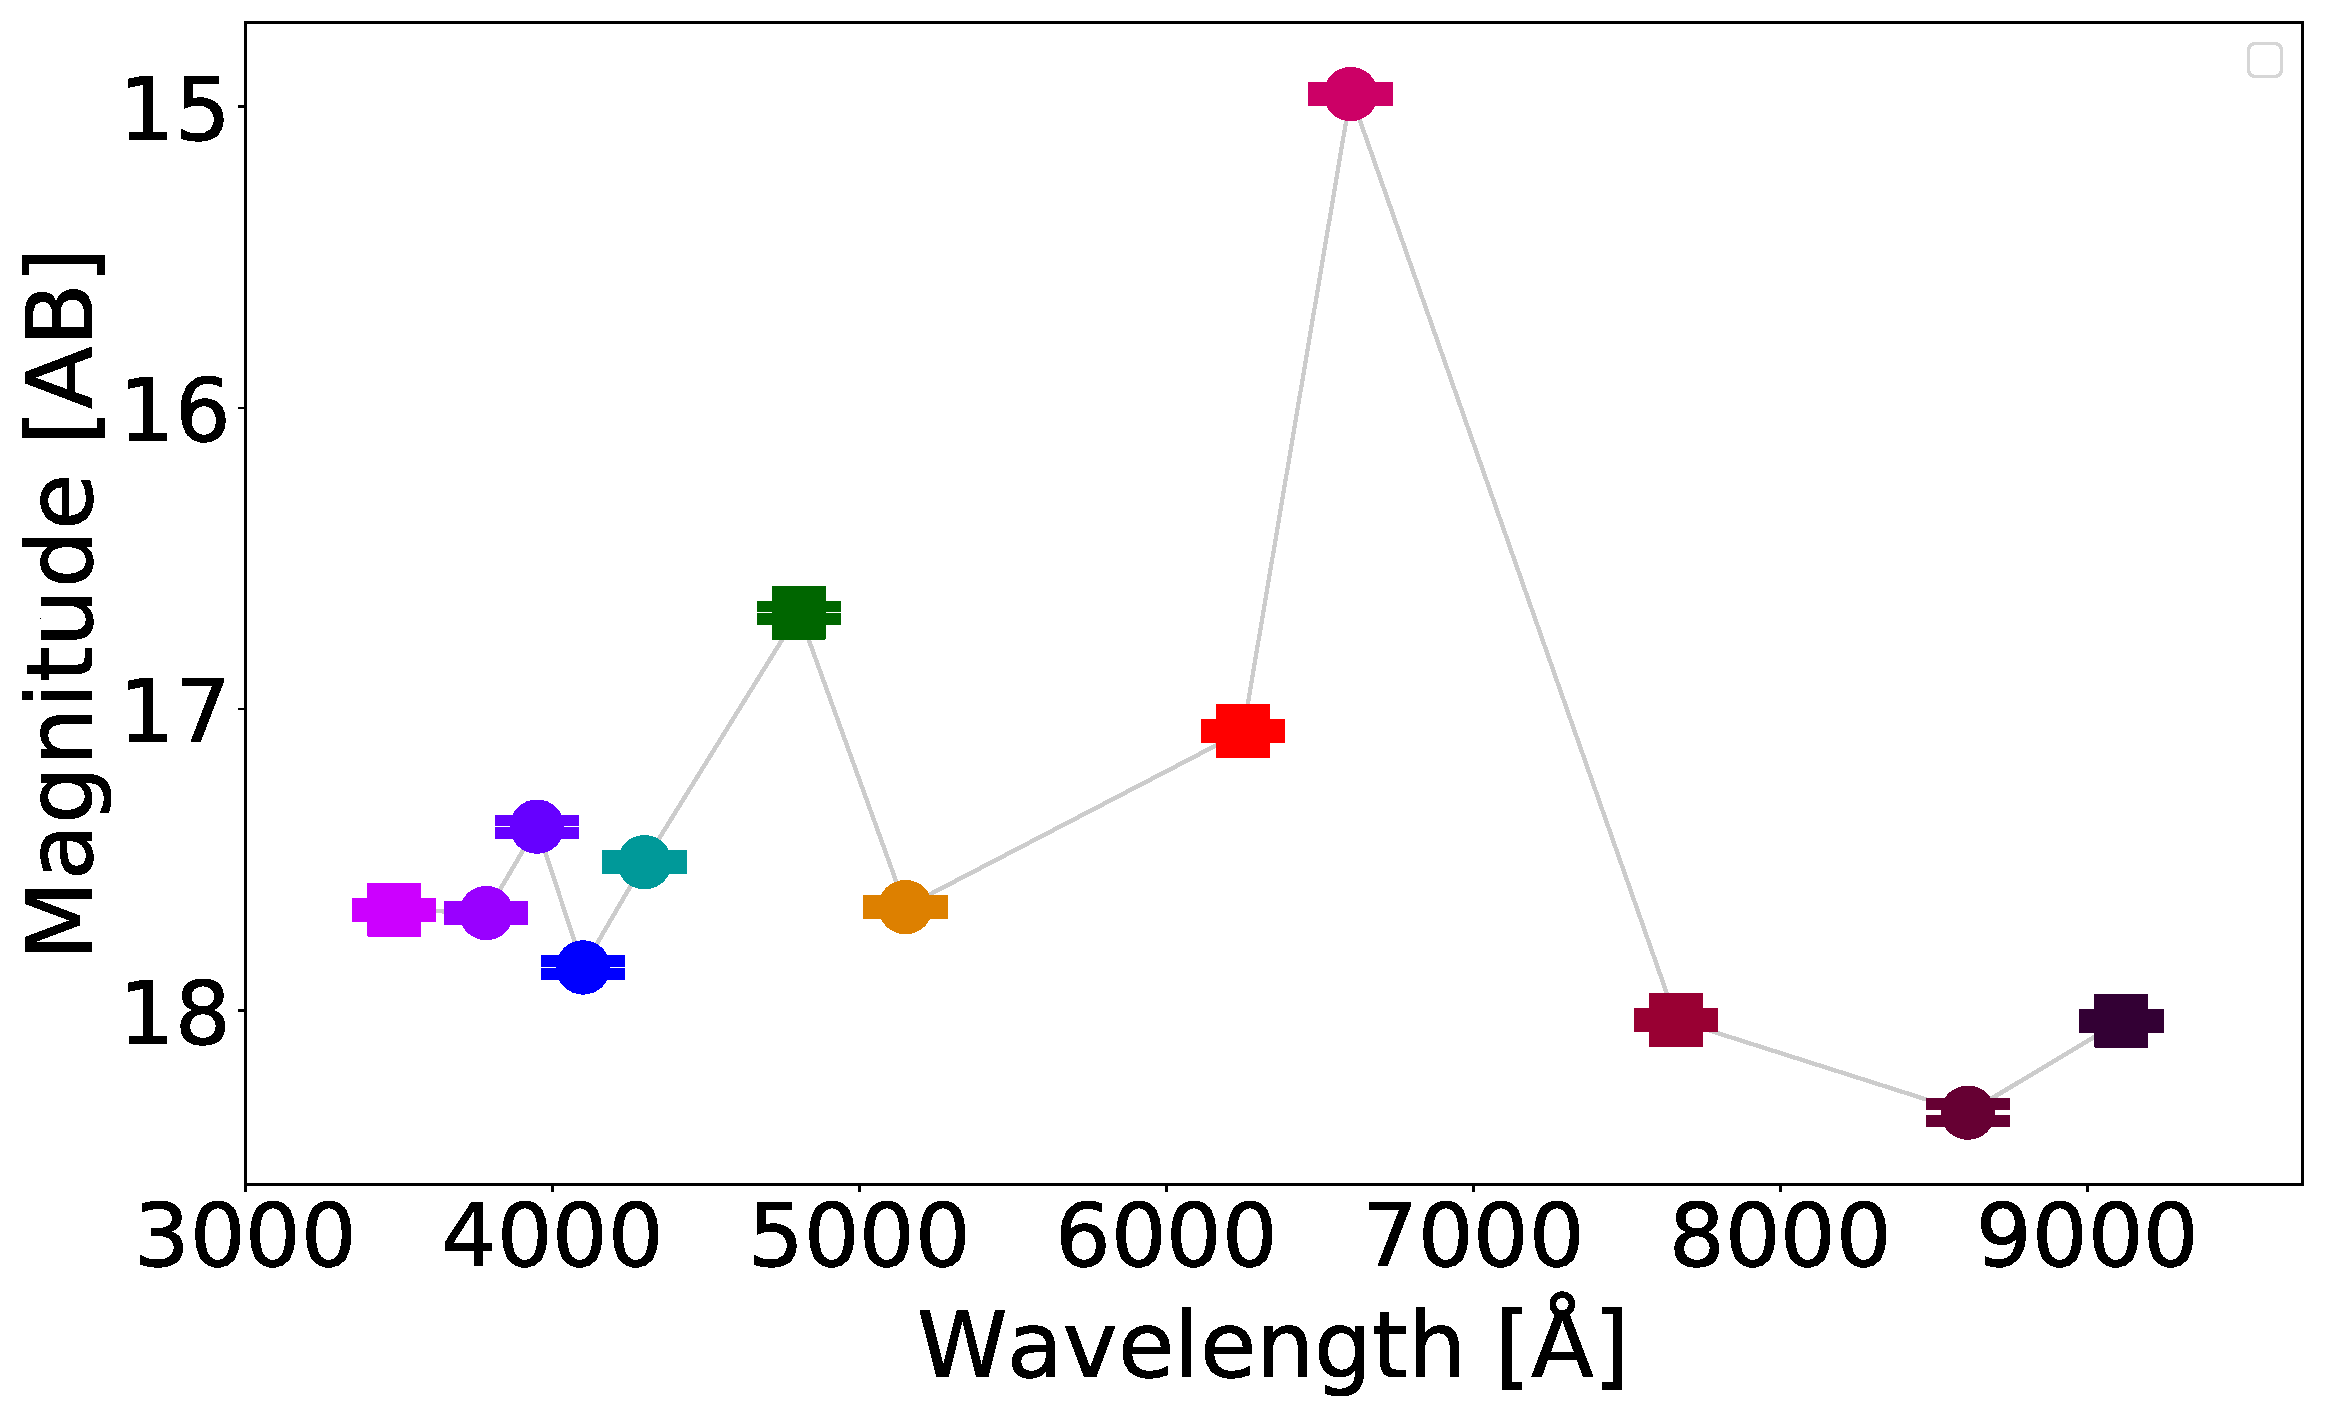
\includegraphics[width=0.3\linewidth, clip]{photopectrum_splus_MC0093-085620_aper.pdf} & 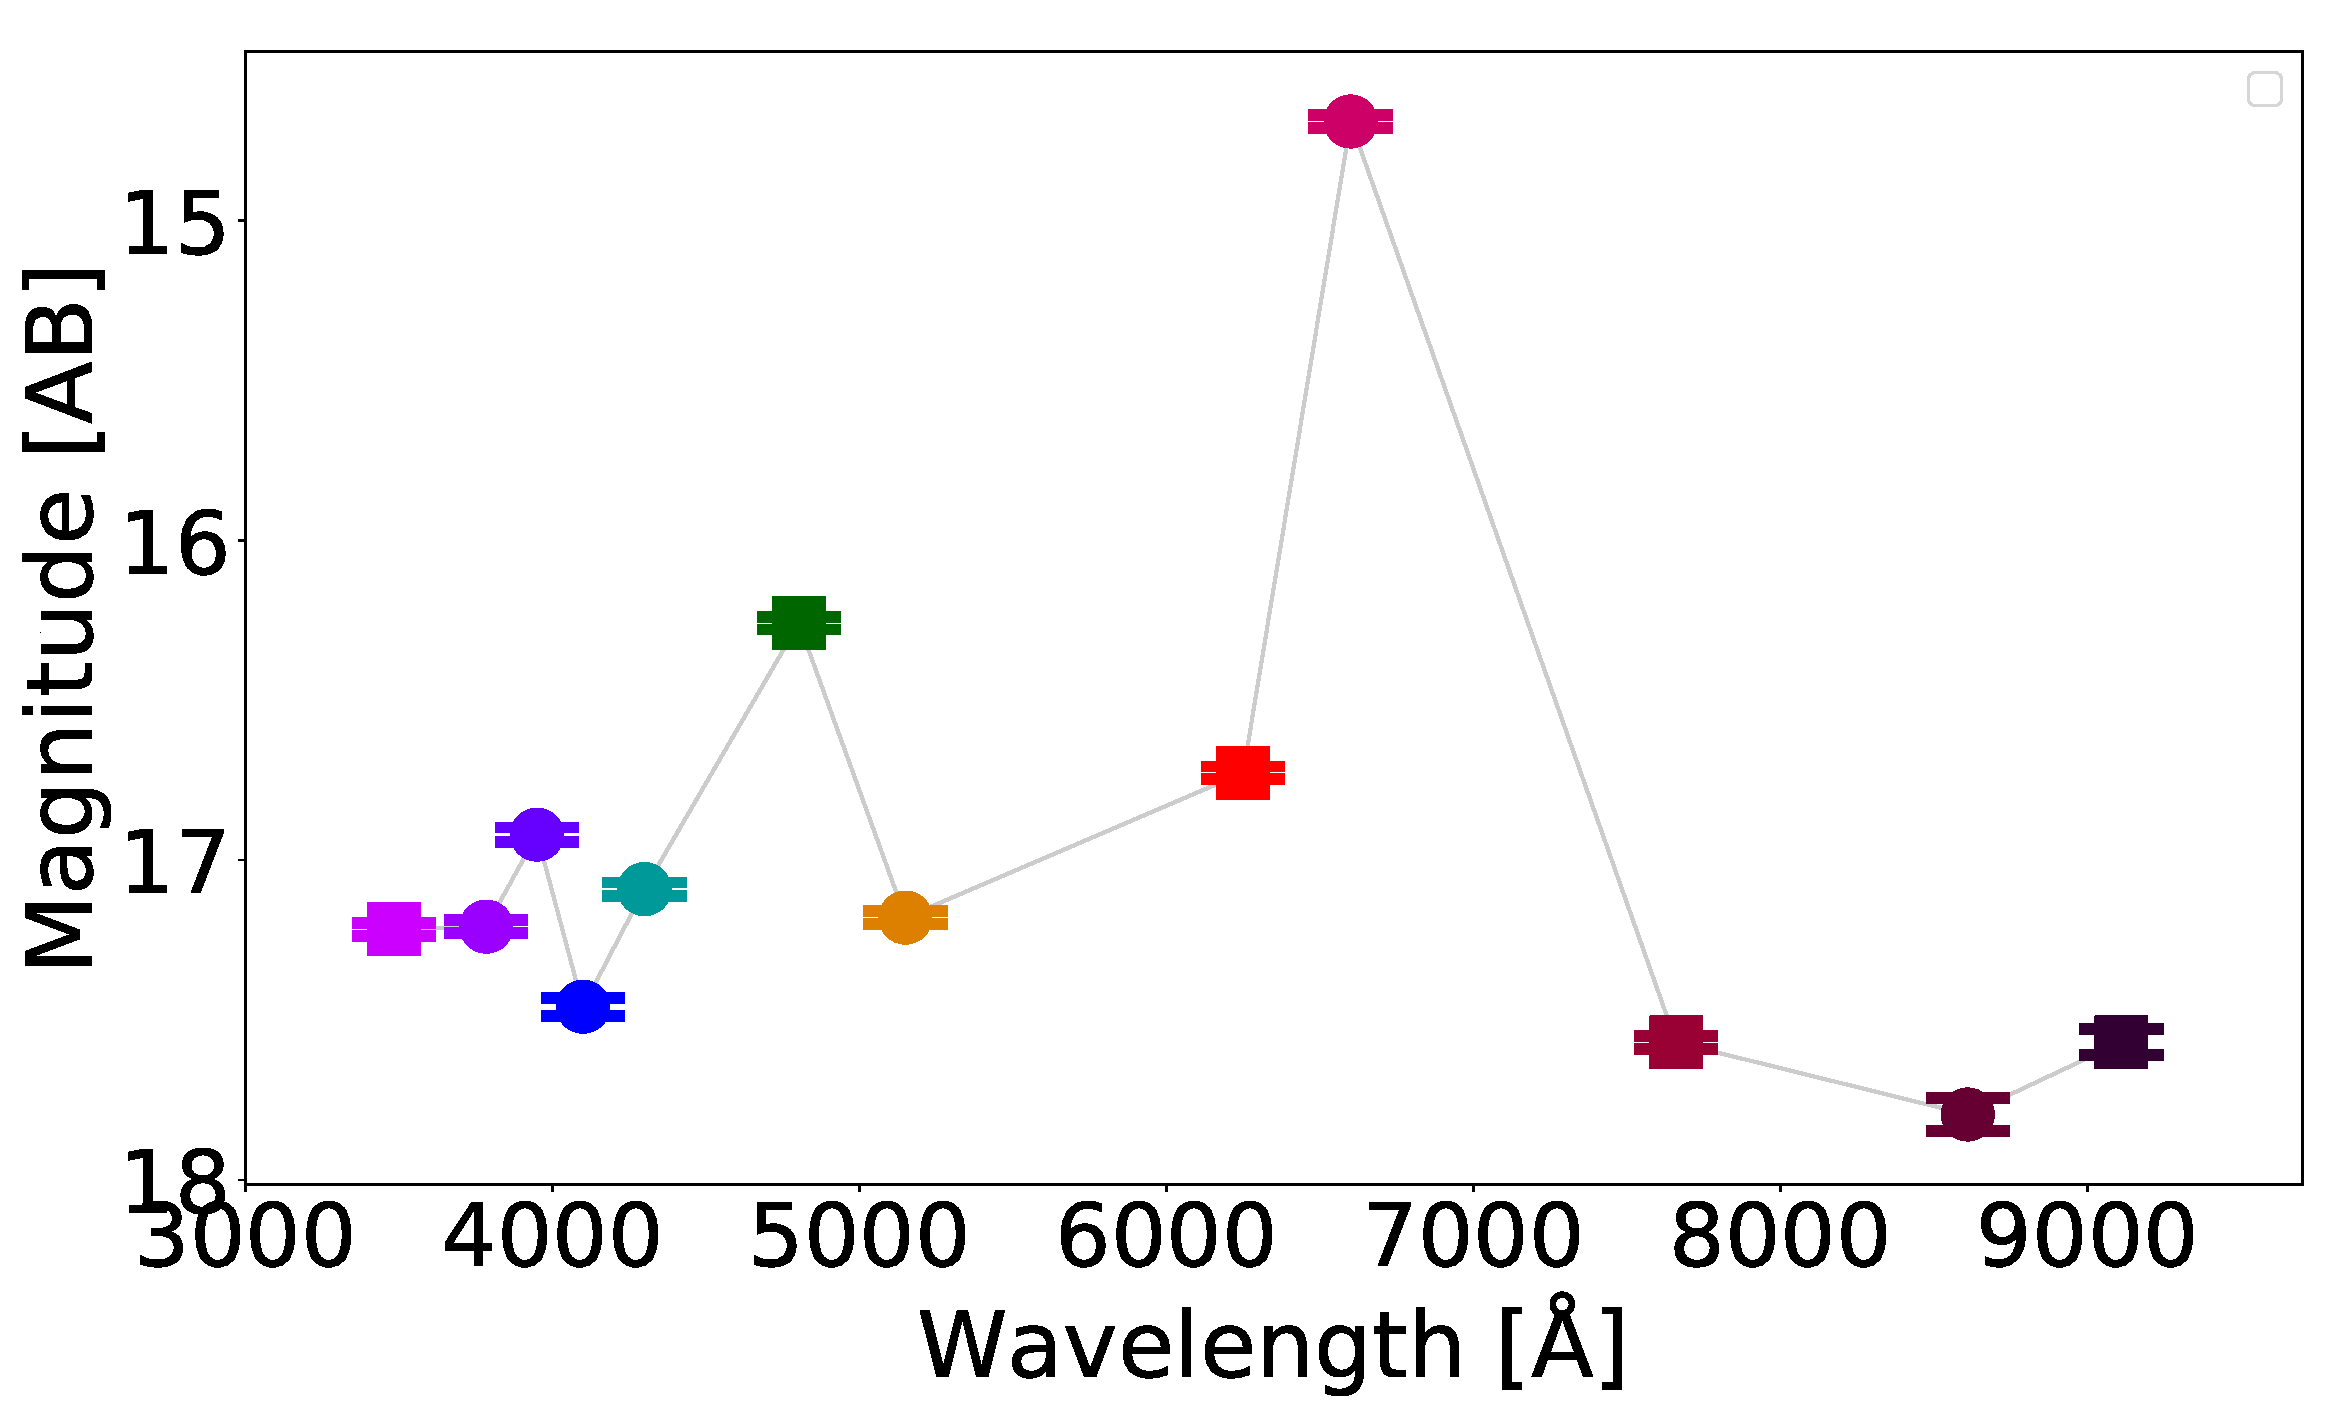
\includegraphics[width=0.3\linewidth, clip]{photopectrum_splus_MC0093-085620_auto.pdf} & 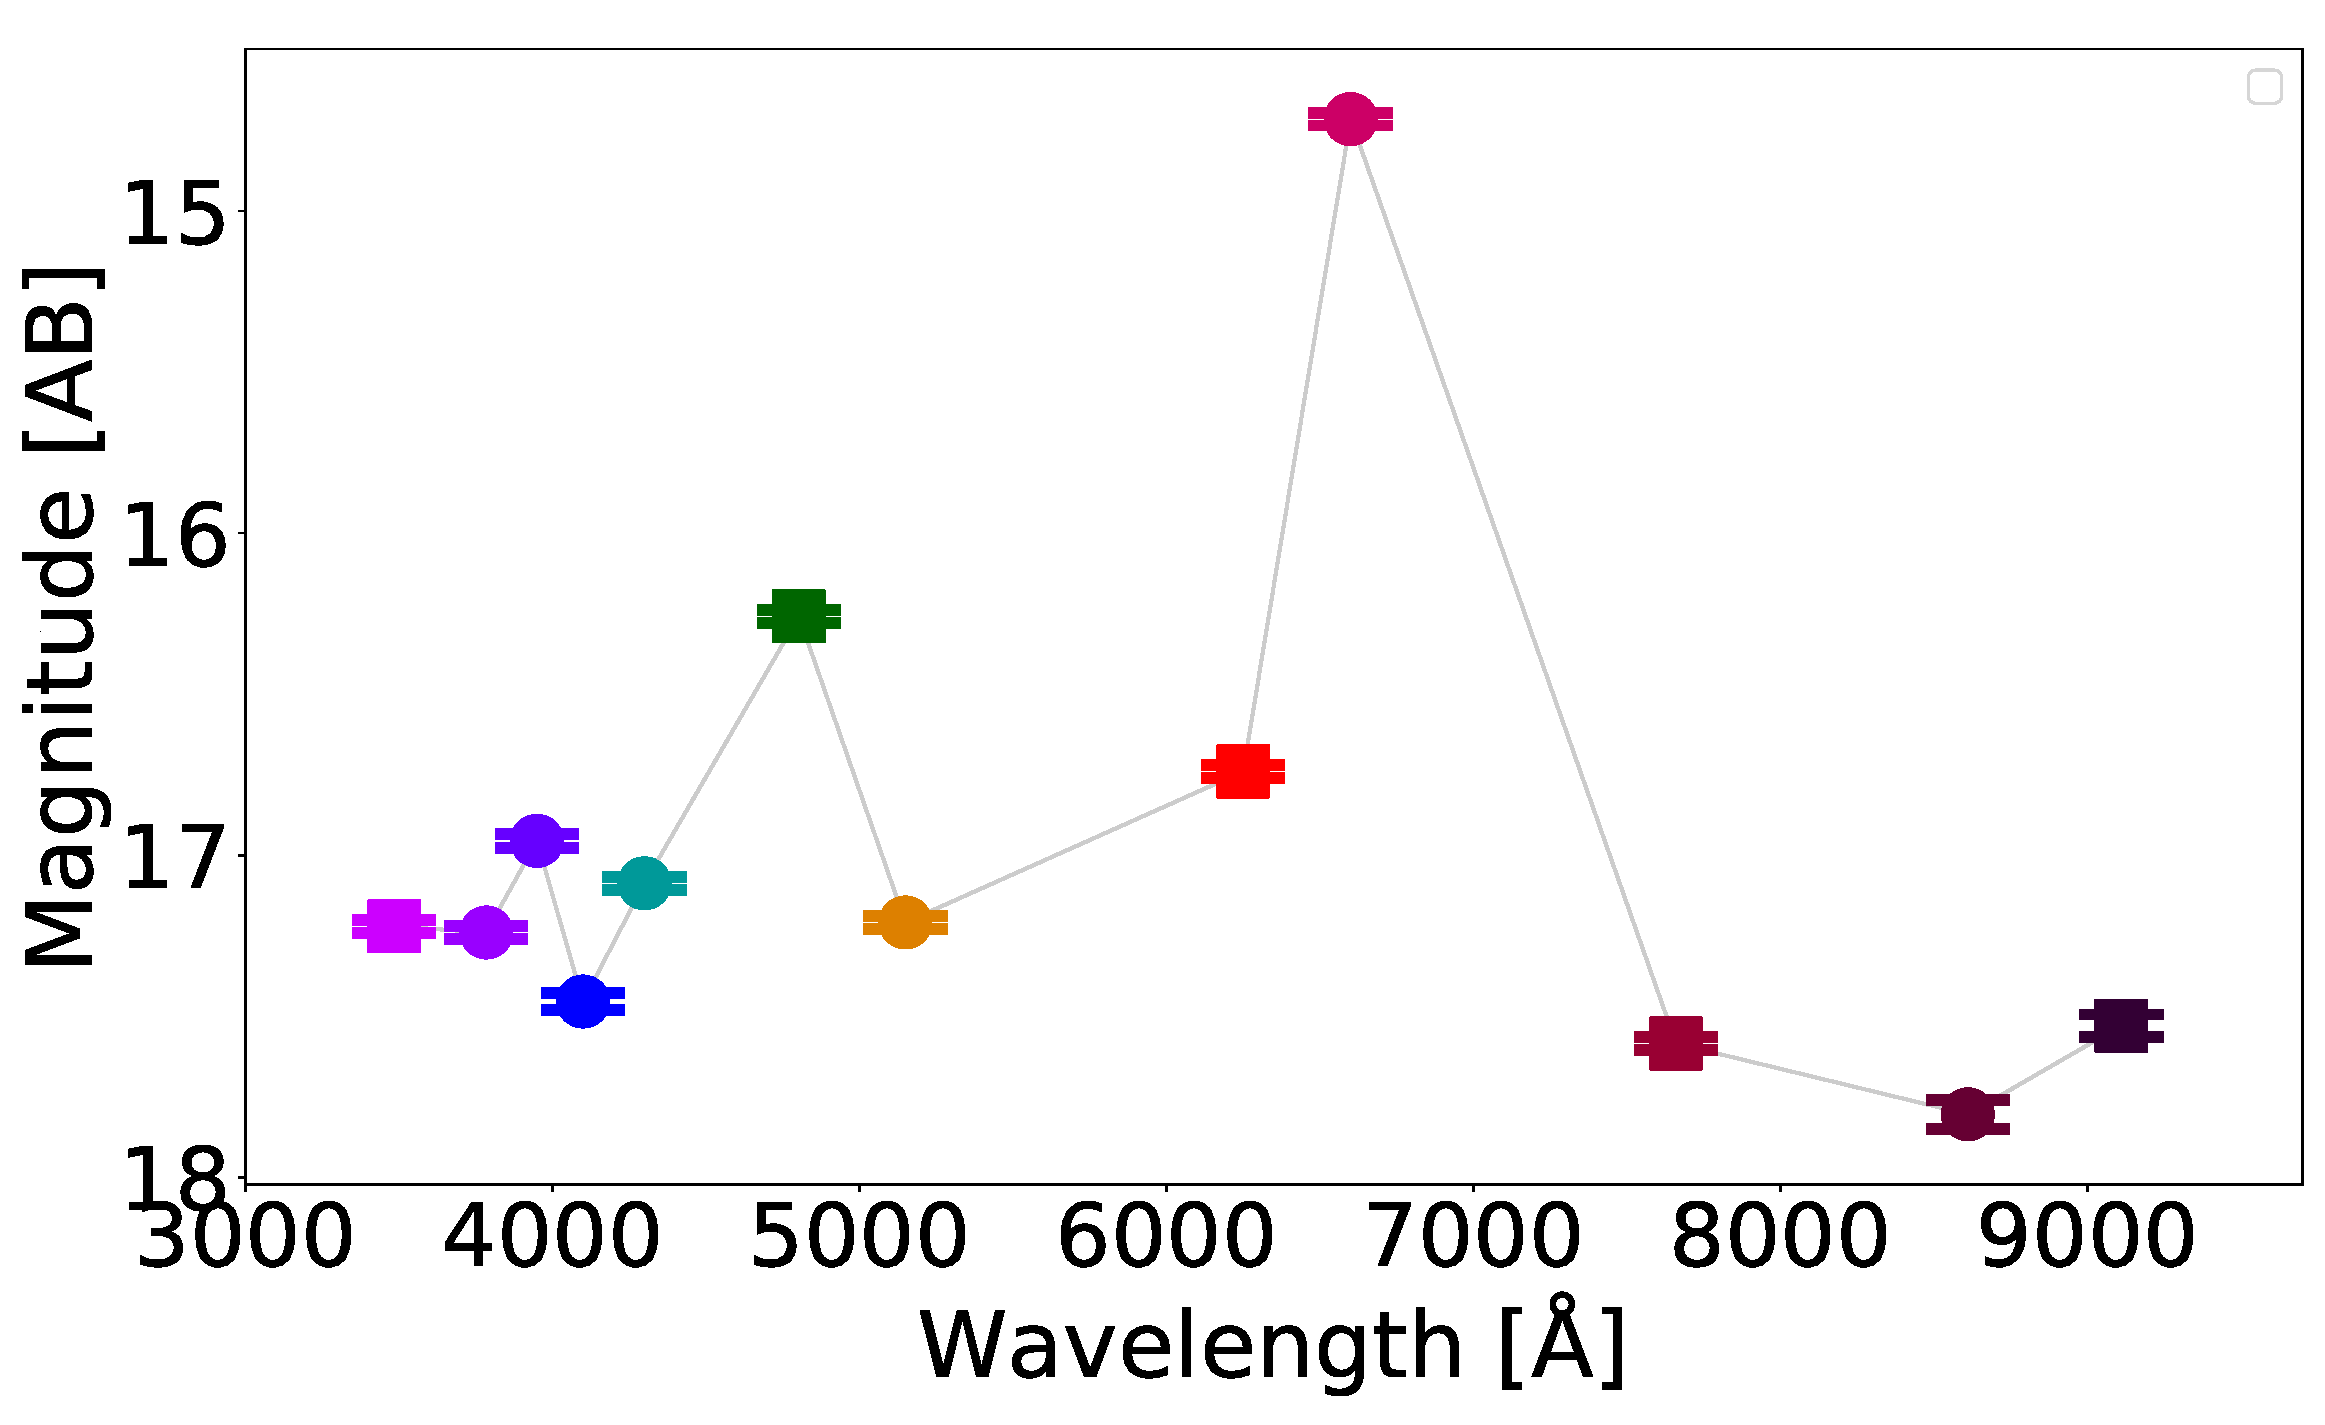
\includegraphics[width=0.3\linewidth, clip]{photopectrum_splus_MC0093-085620_petro.pdf} \\
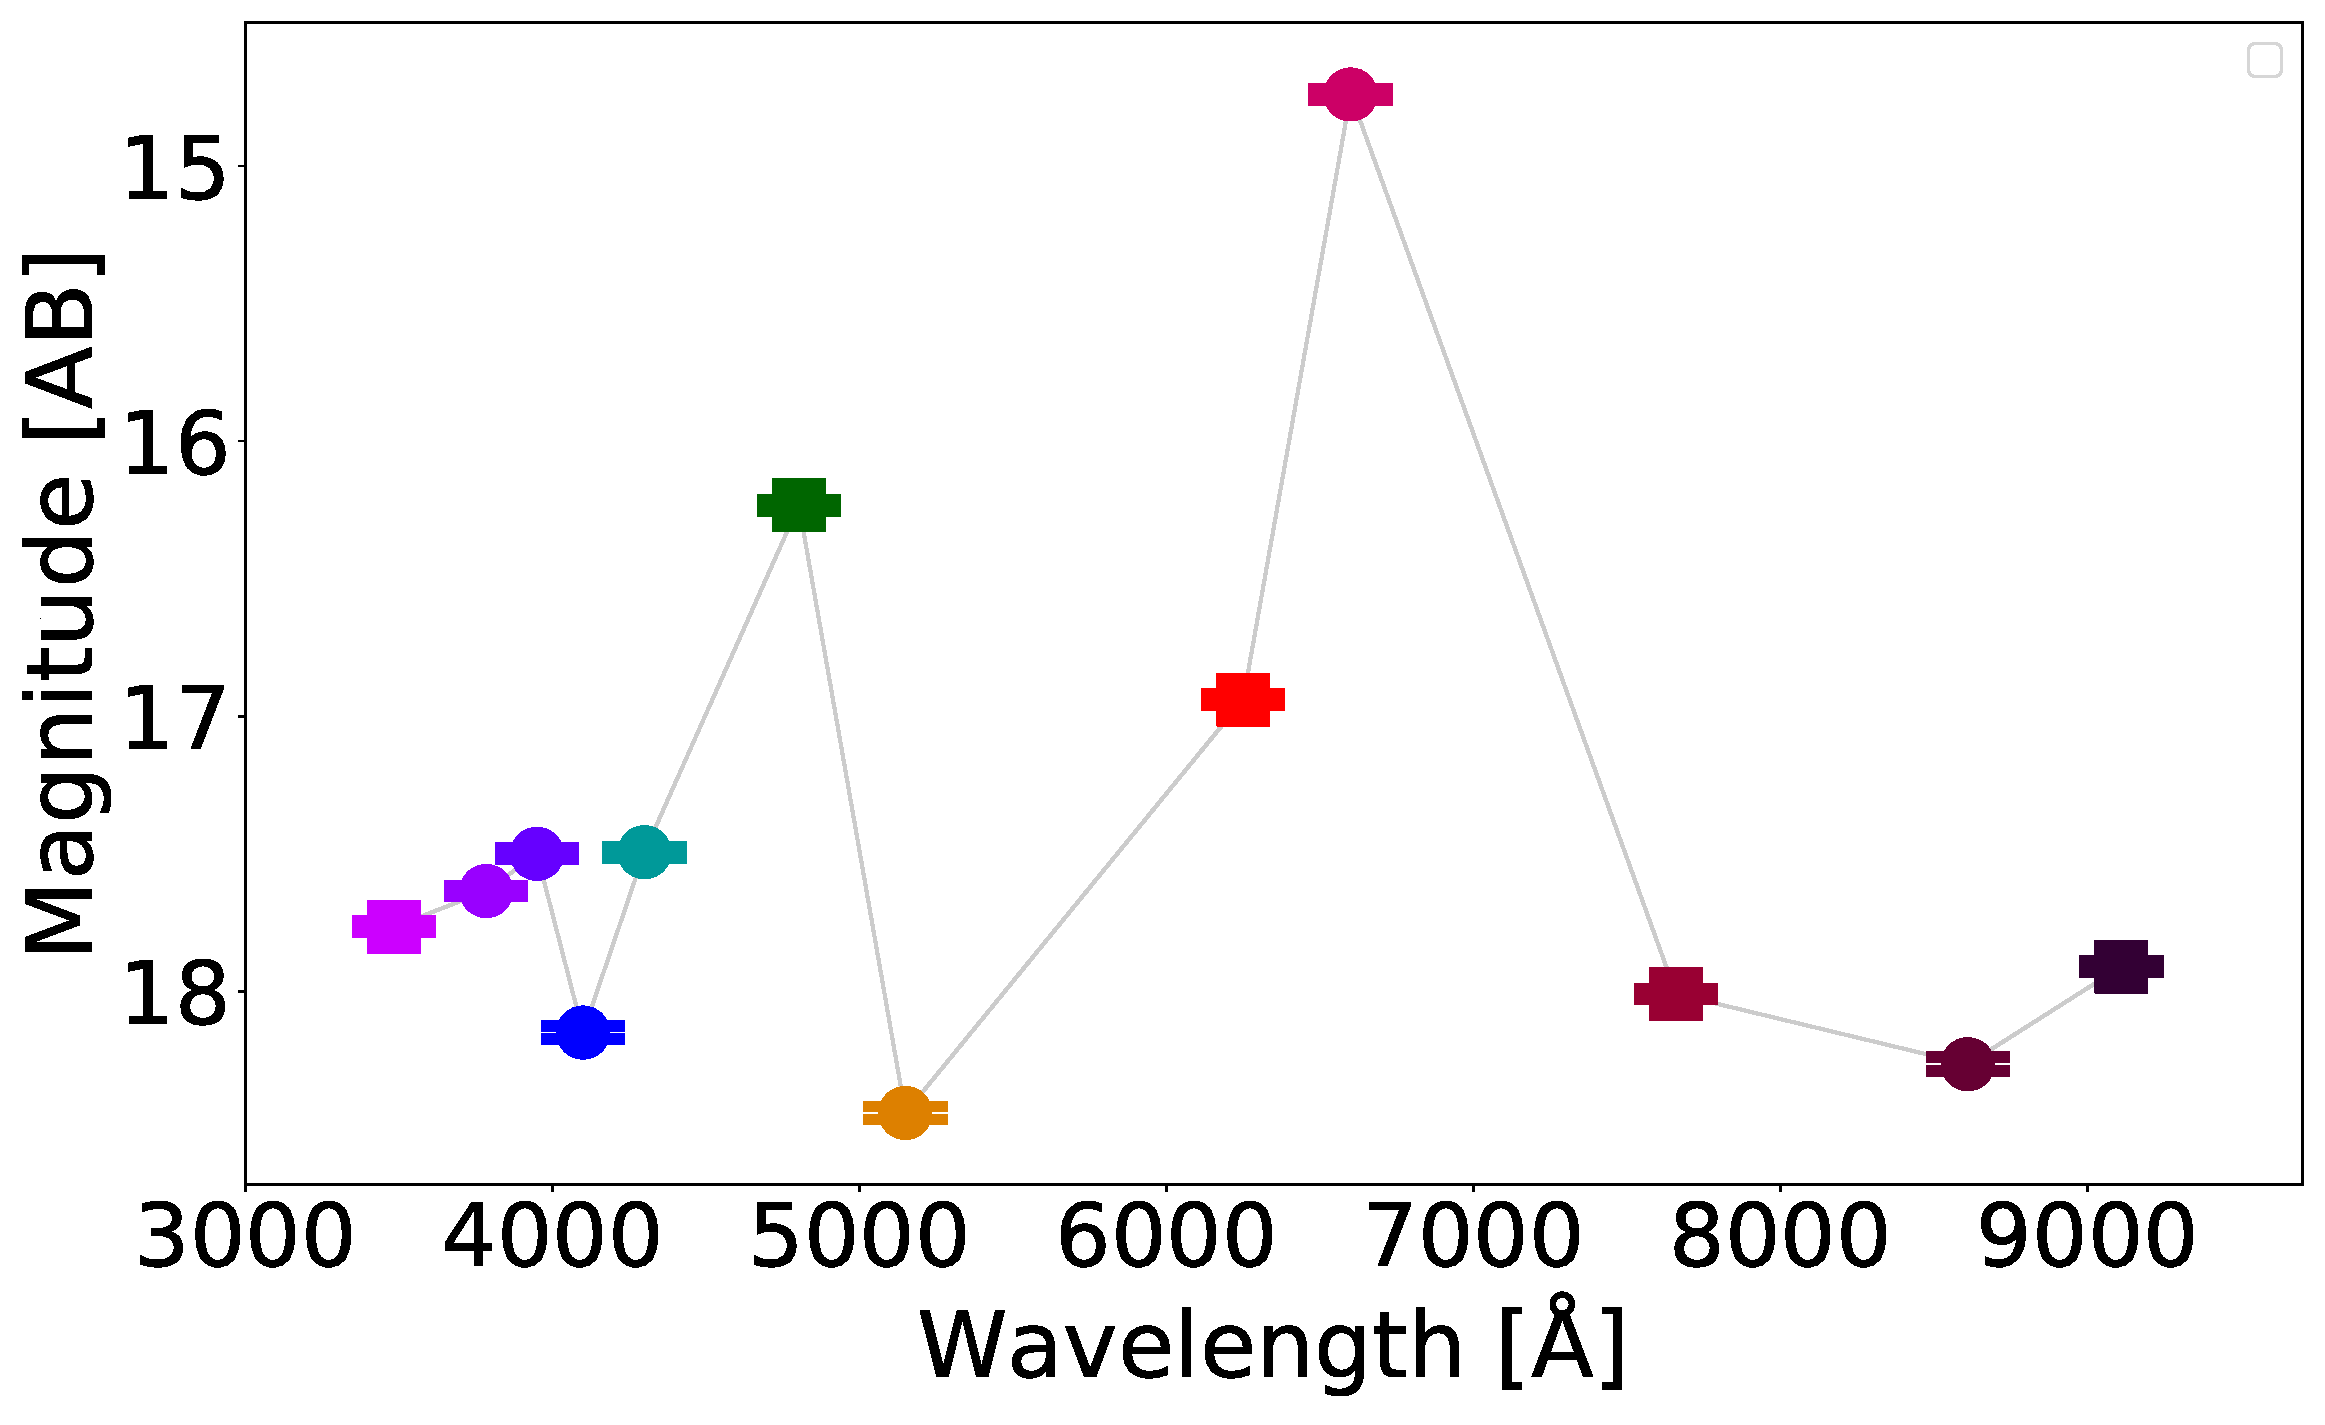
\includegraphics[width=0.3\linewidth, clip]{photopectrum_splus_MC0093-295870_aper.pdf} & 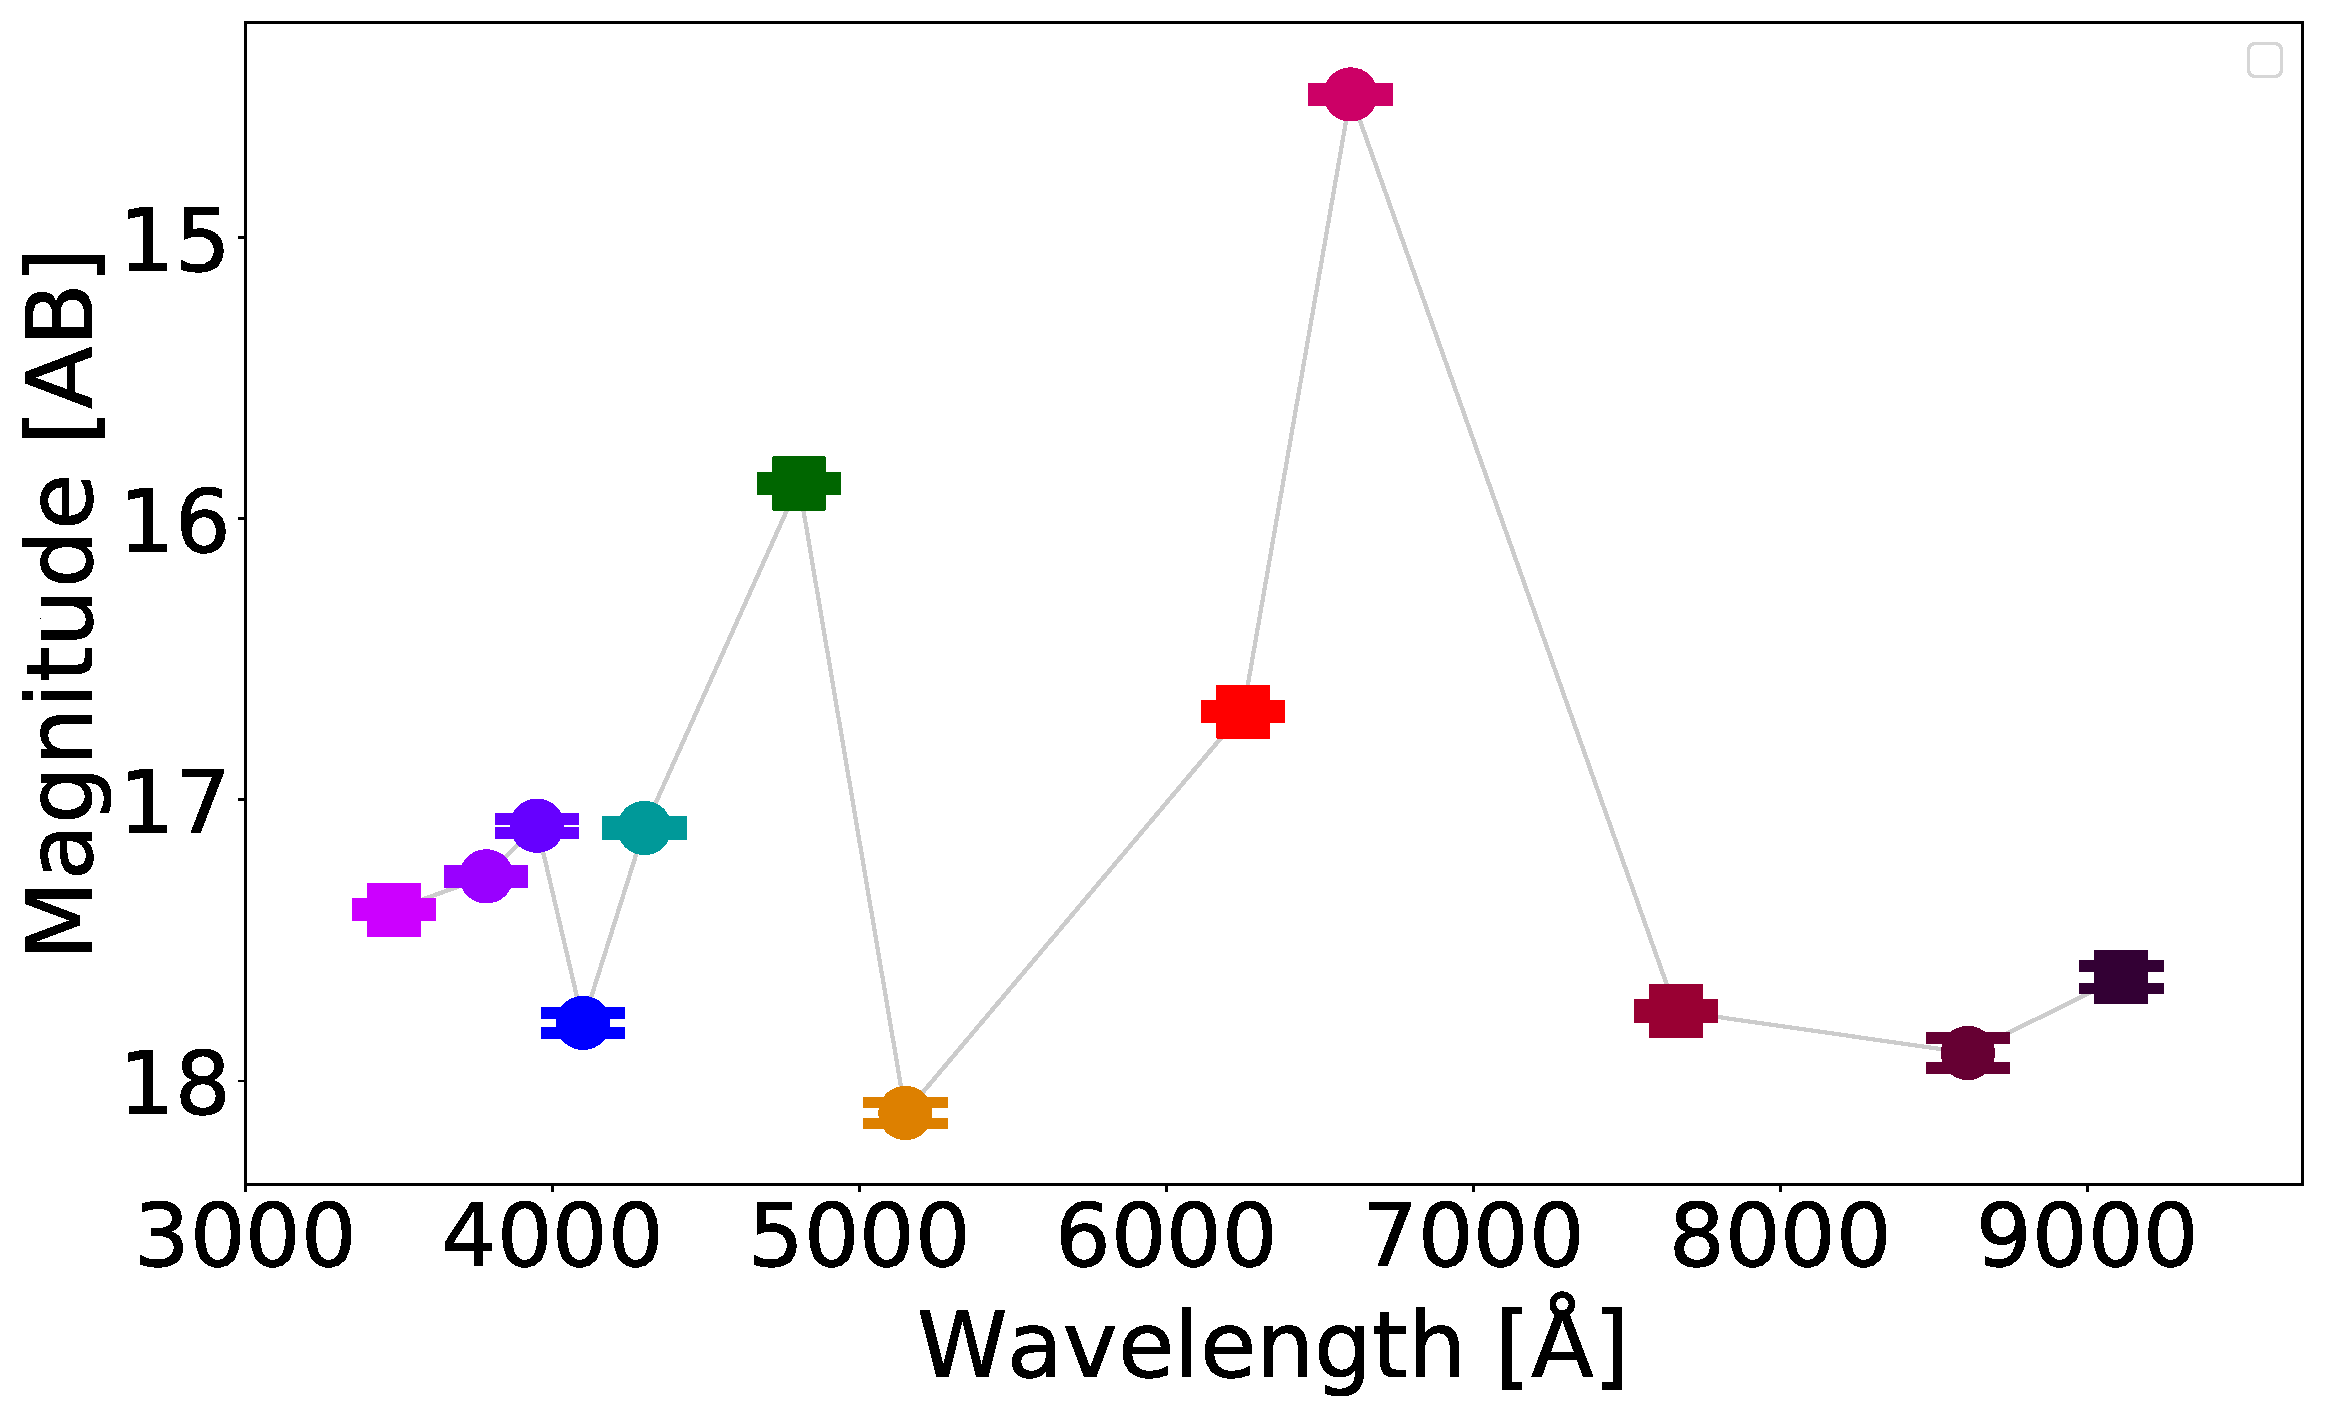
\includegraphics[width=0.3\linewidth, clip]{photopectrum_splus_MC0093-295870_auto.pdf} & 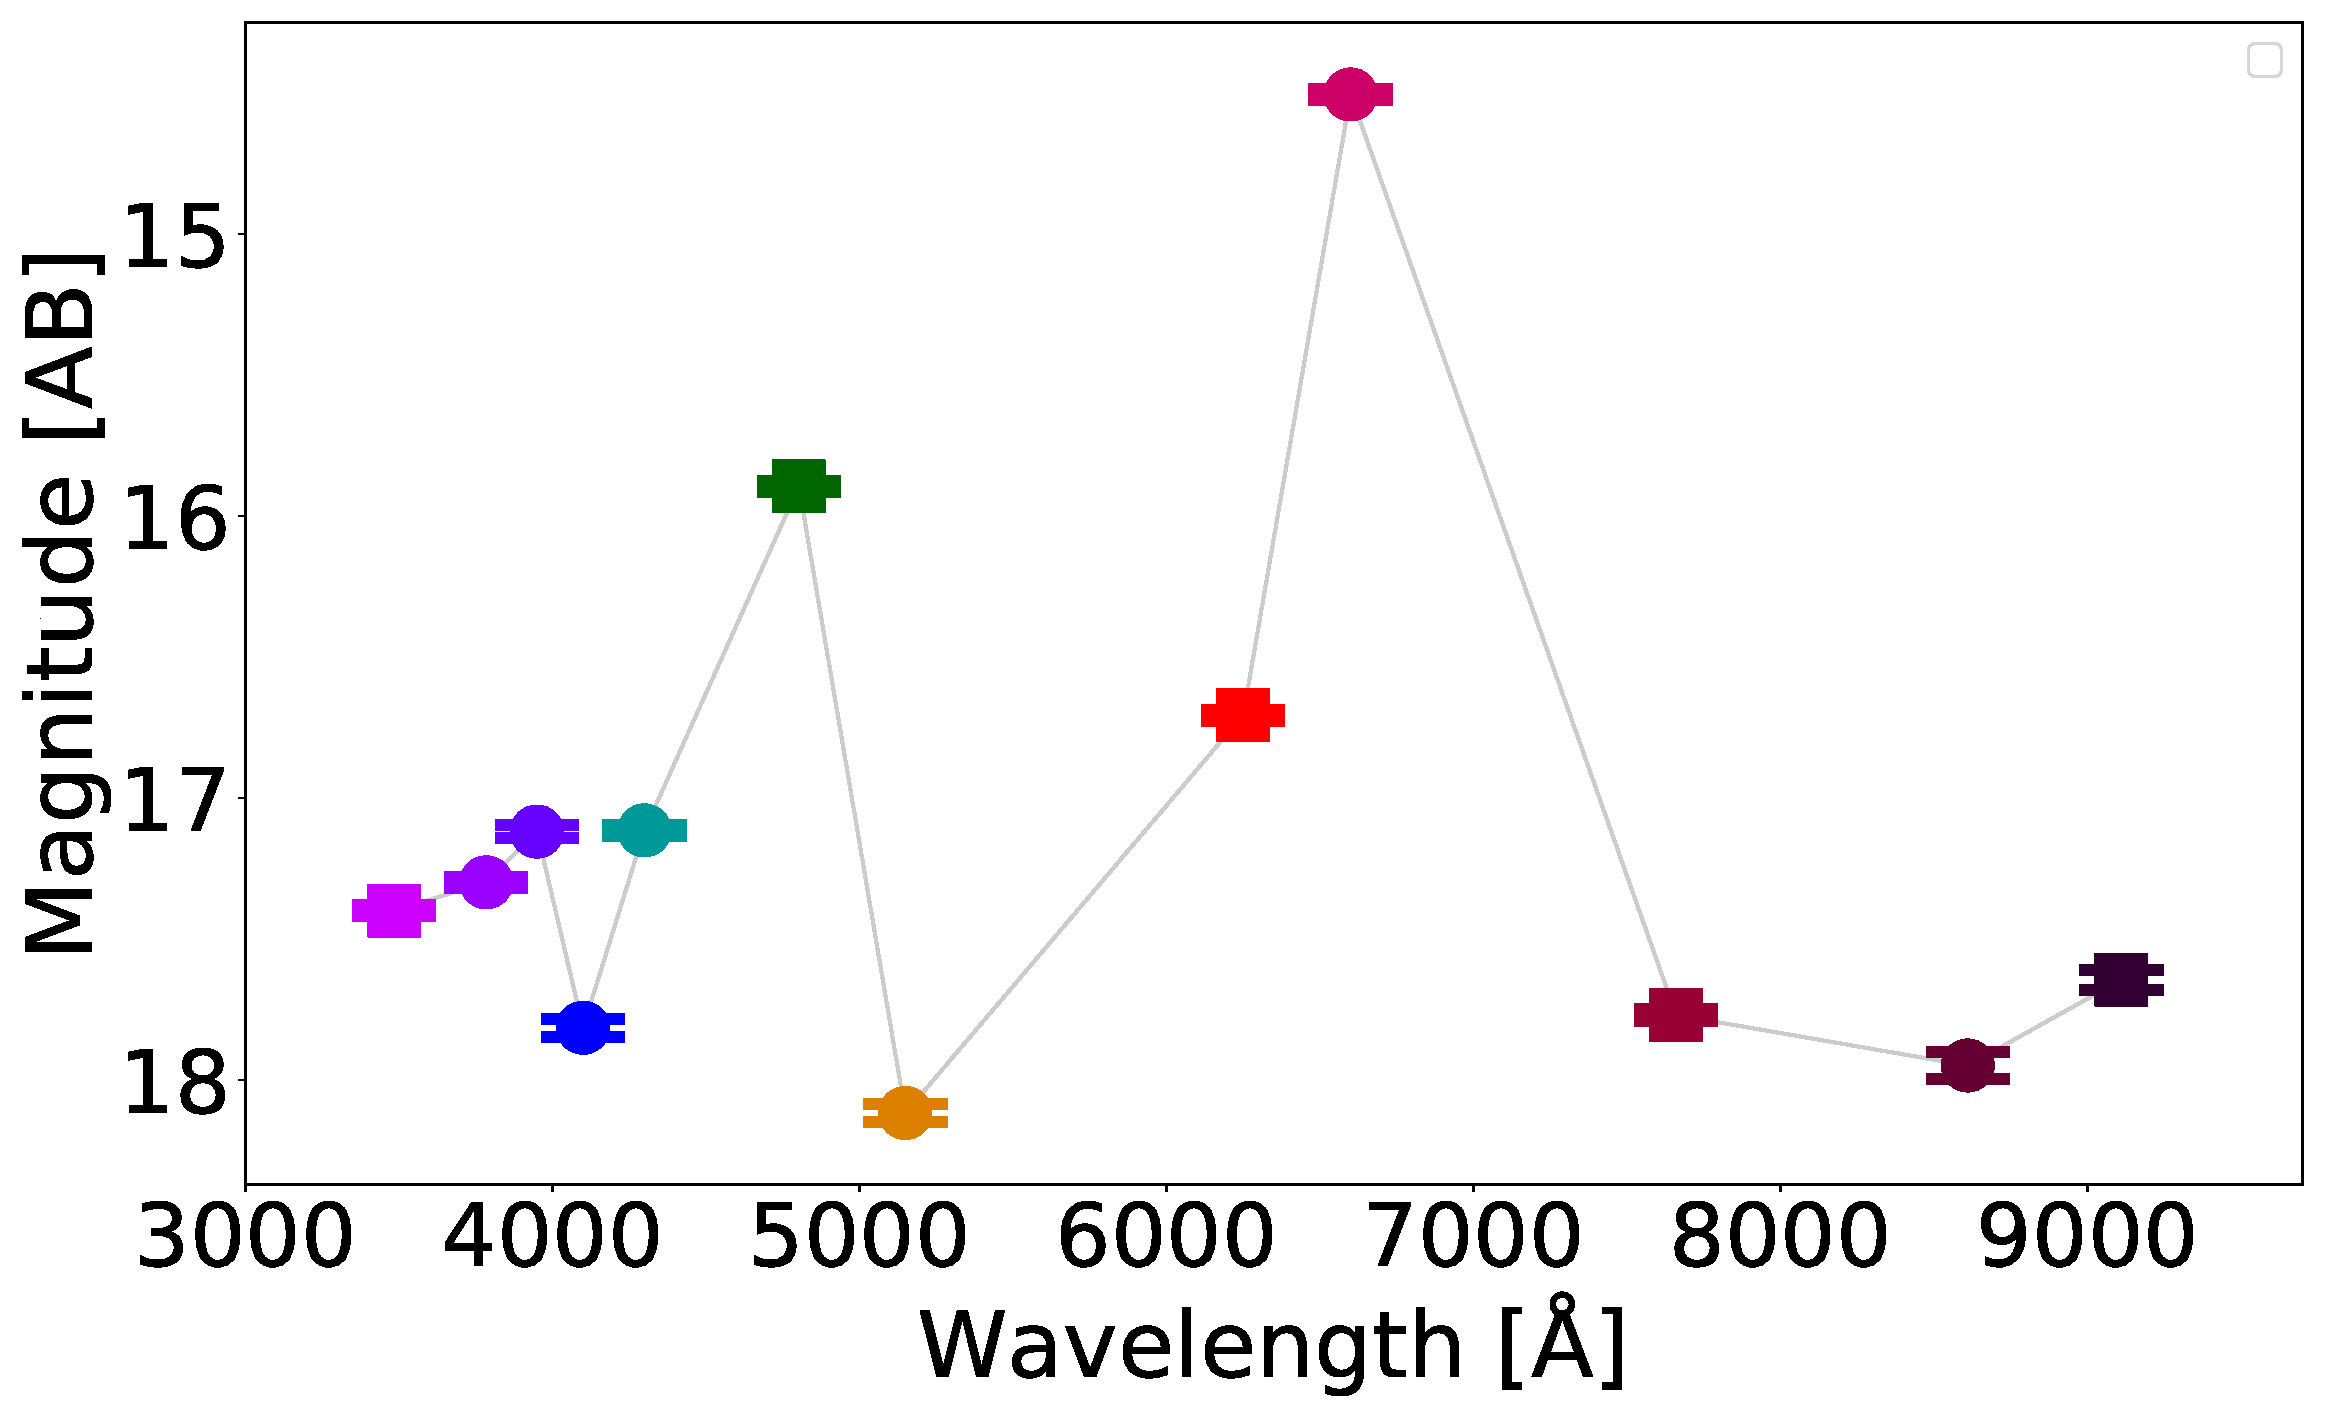
\includegraphics[width=0.3\linewidth, clip]{photopectrum_splus_MC0093-295870_petro.pdf} \\
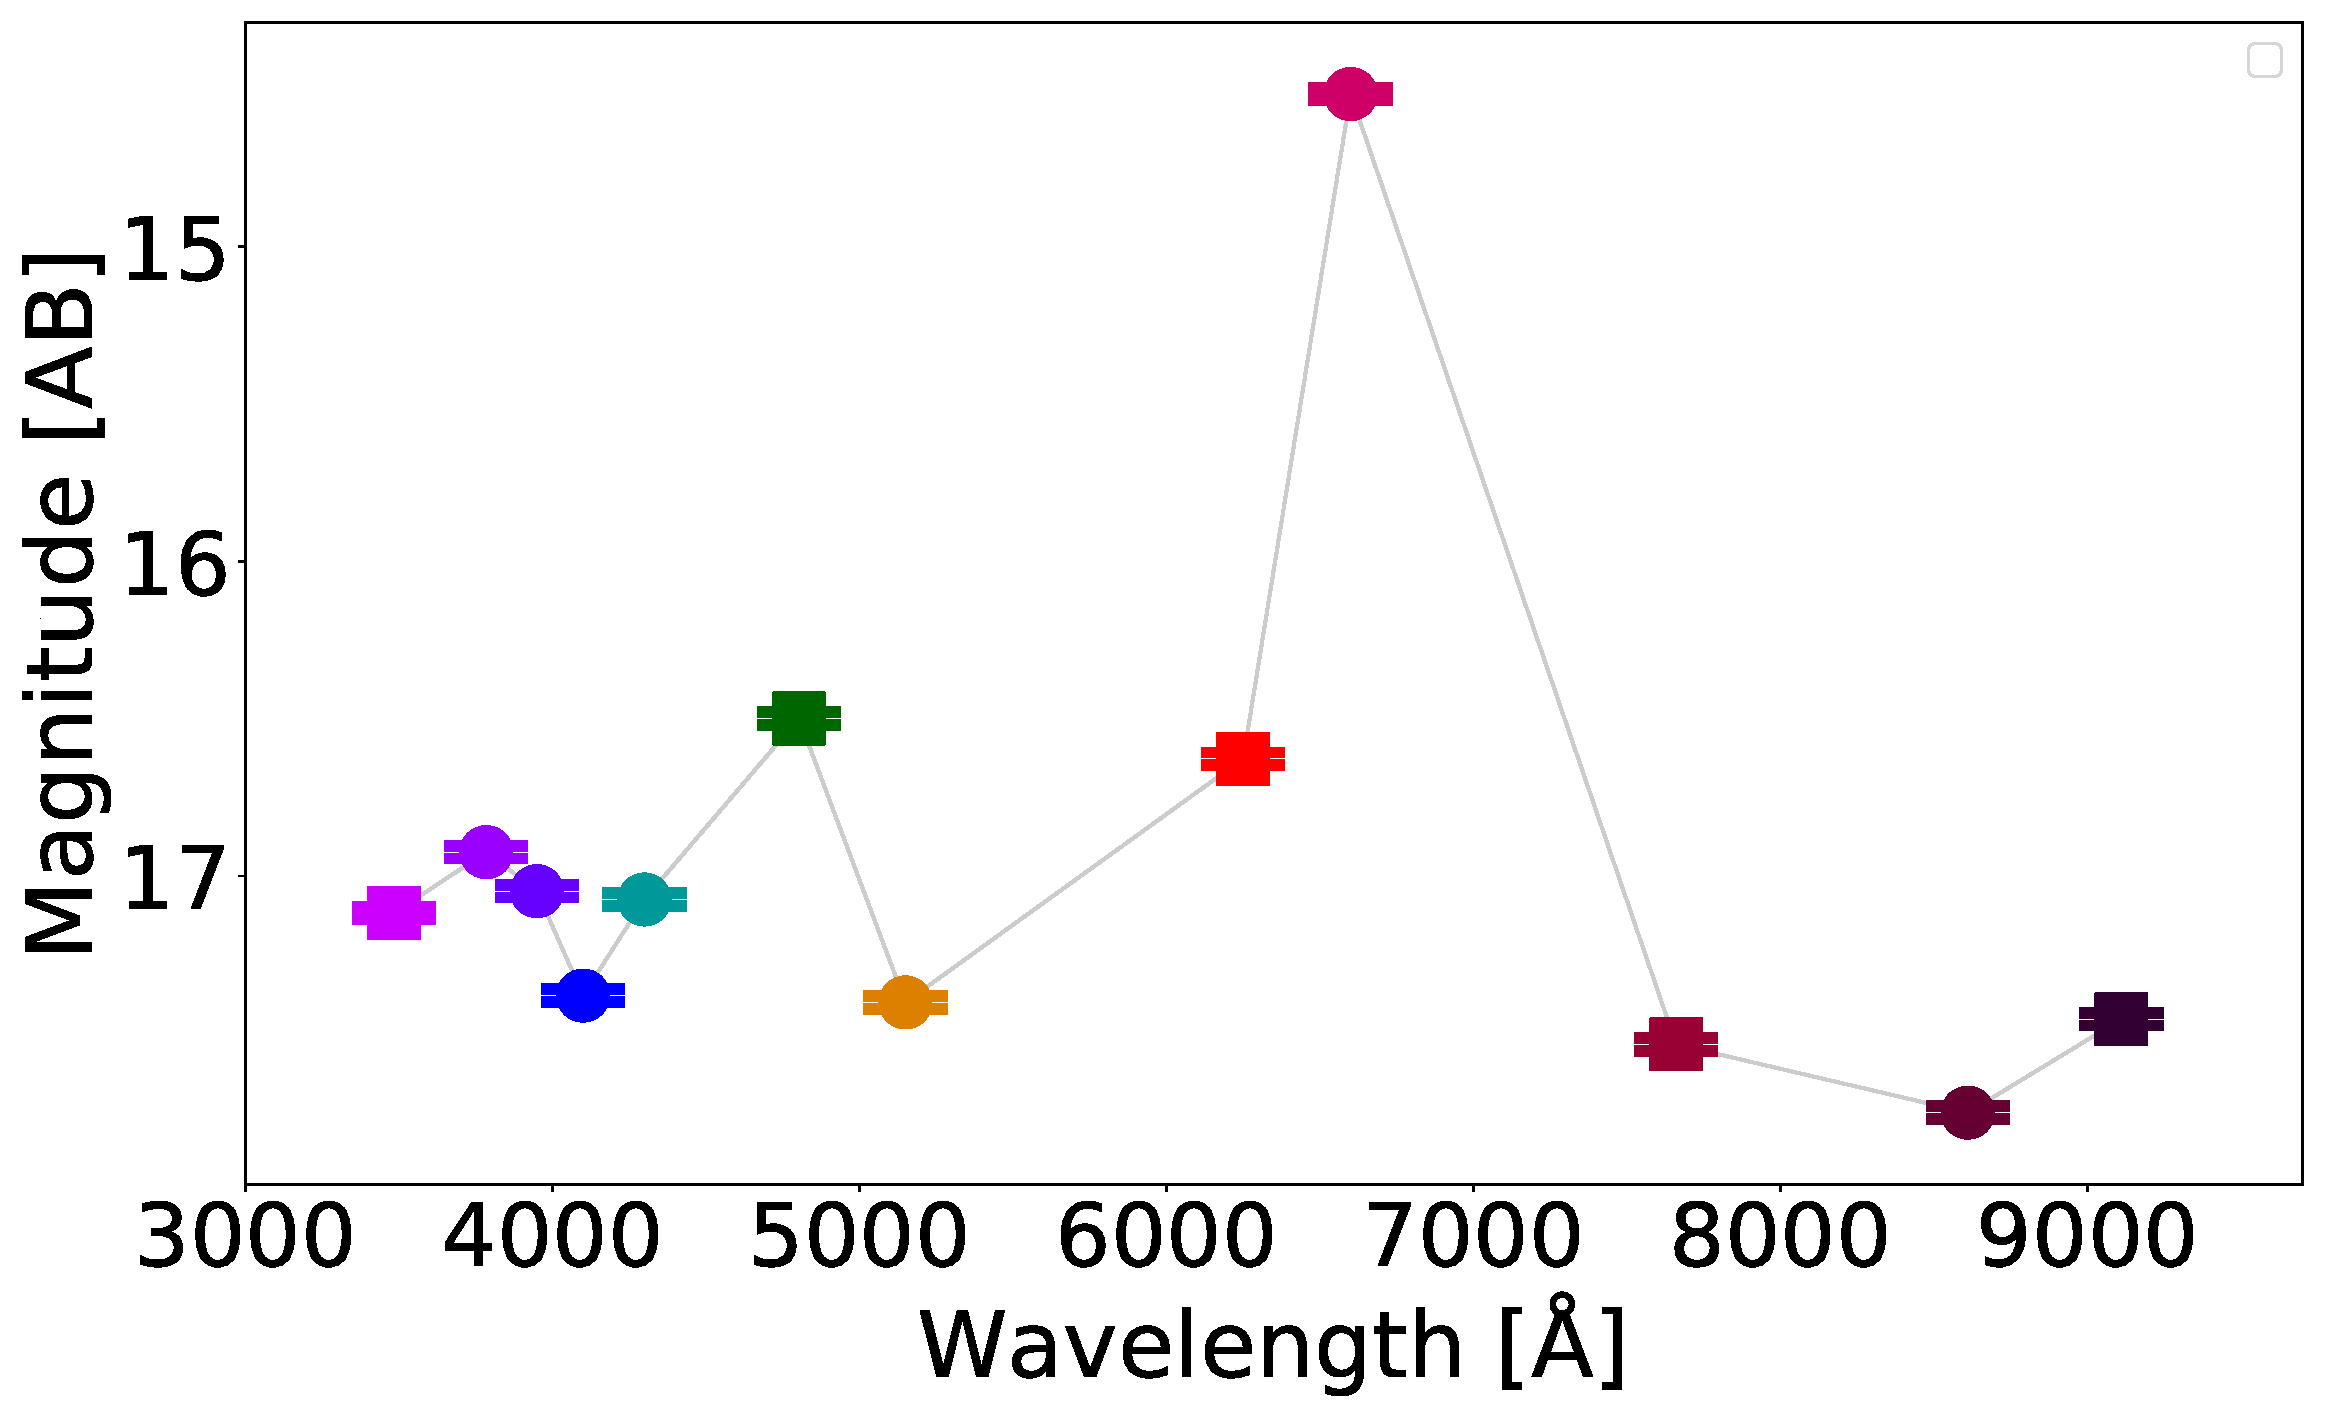
\includegraphics[width=0.3\linewidth, clip]{photopectrum_splus_MC0094-194143_aper.pdf} & 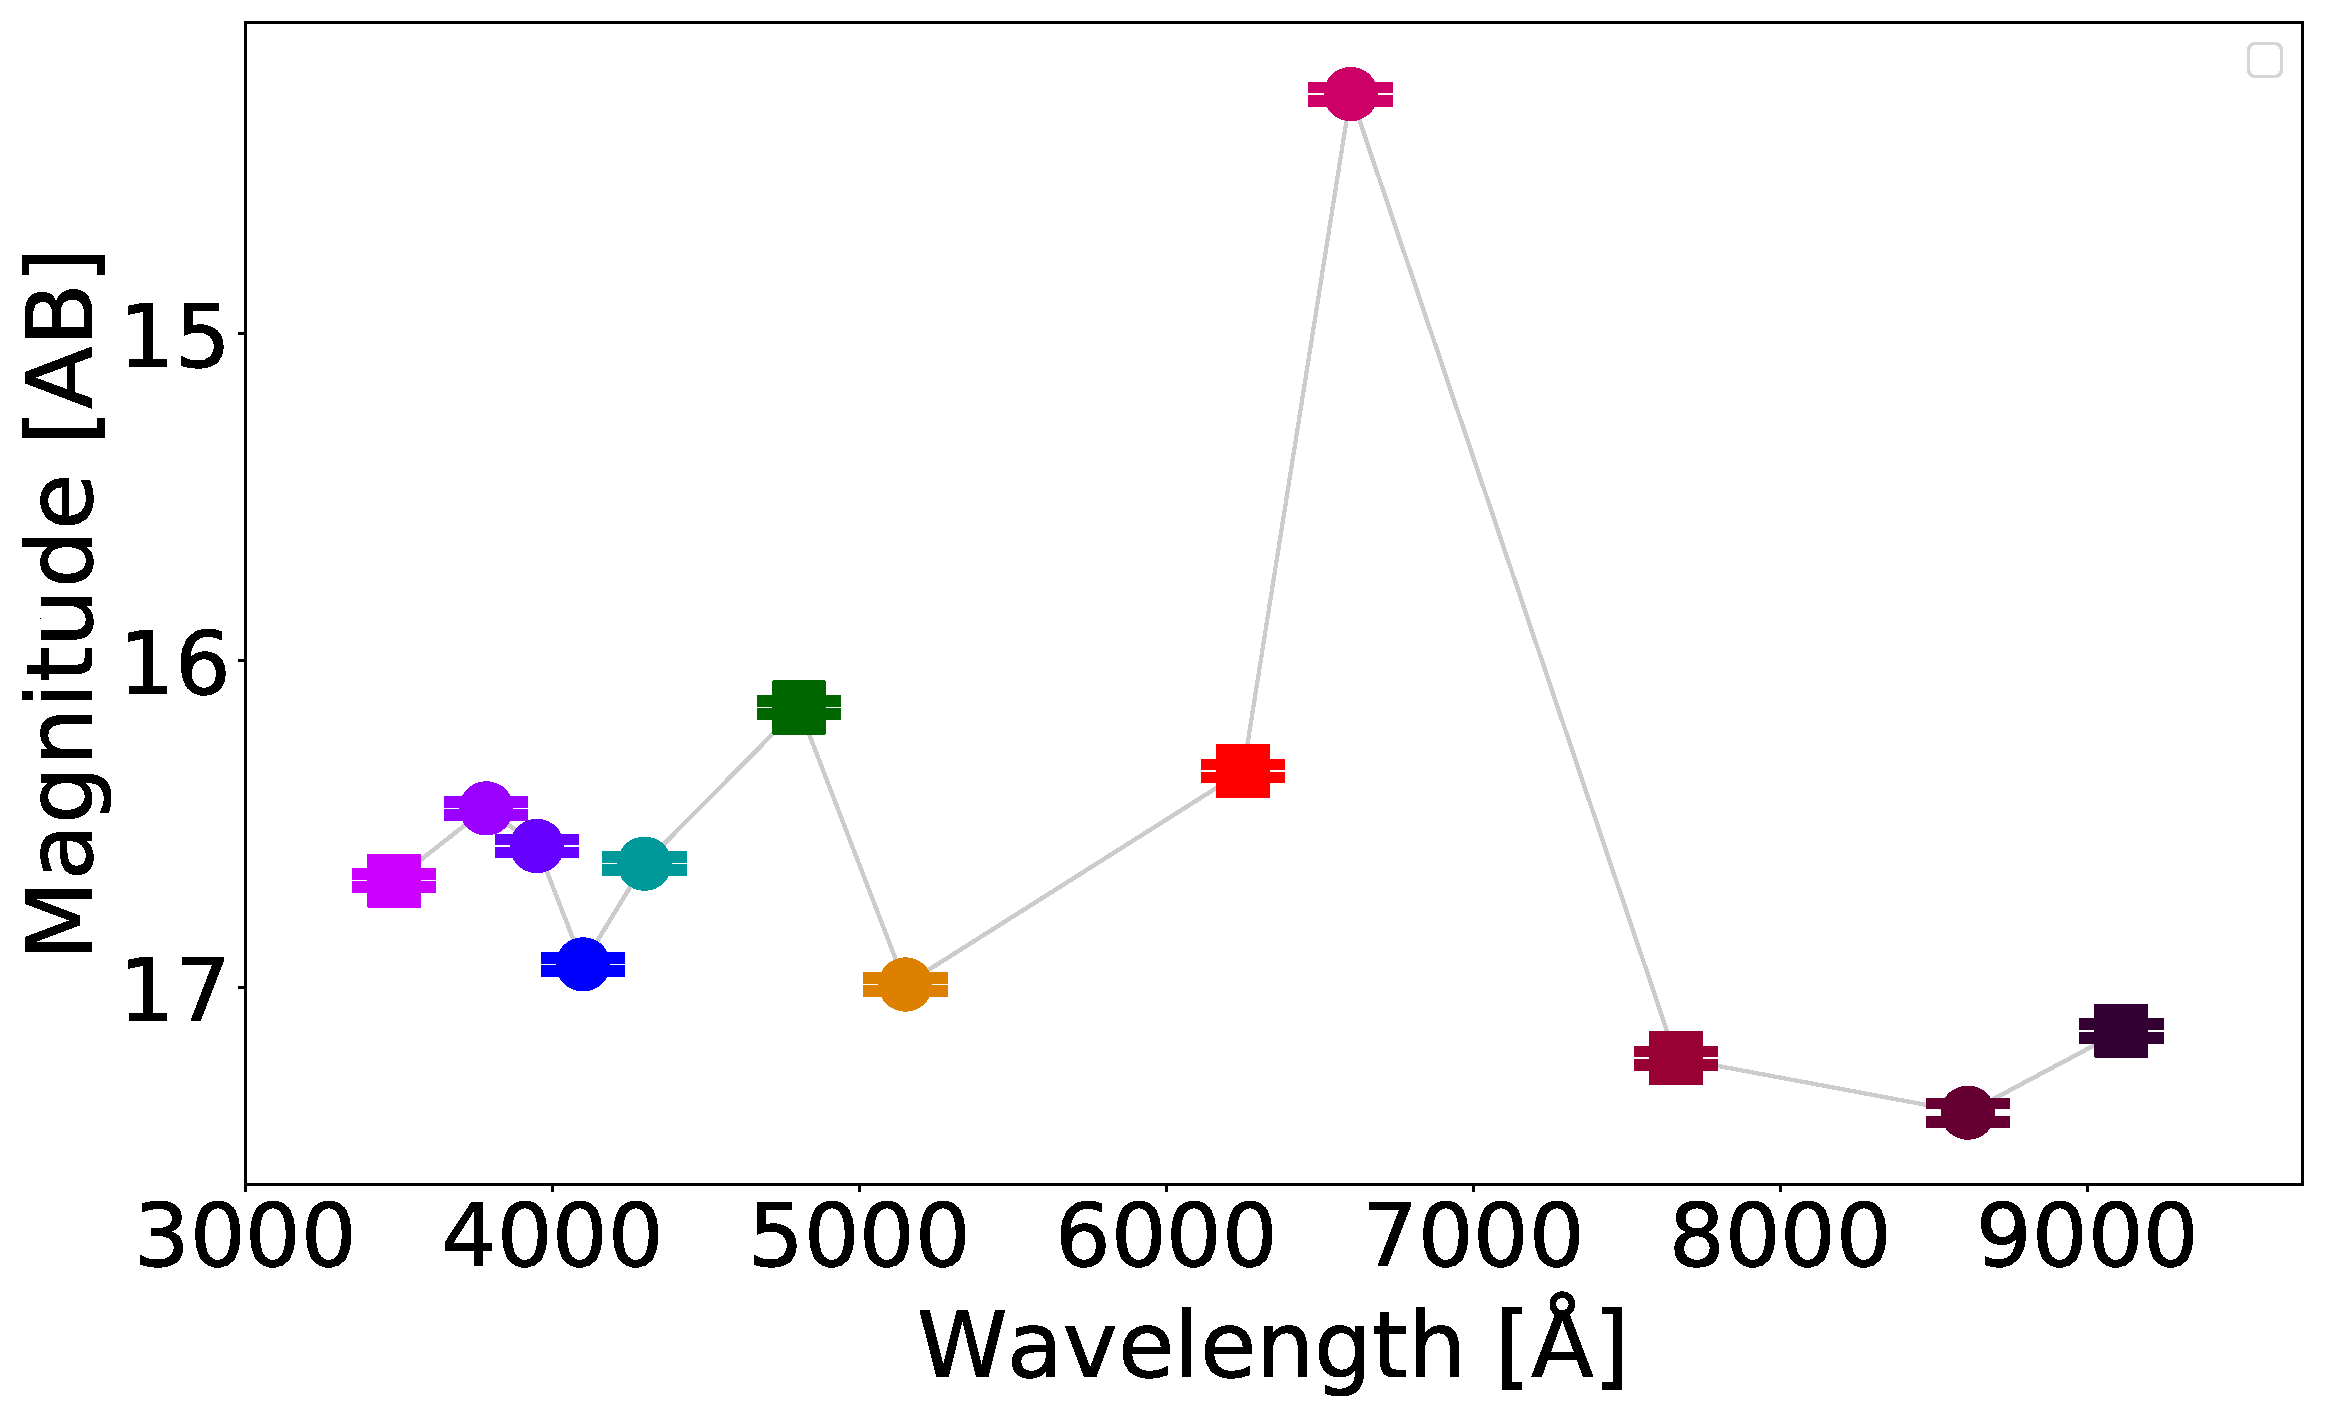
\includegraphics[width=0.3\linewidth, clip]{photopectrum_splus_MC0094-194143_auto.pdf} & 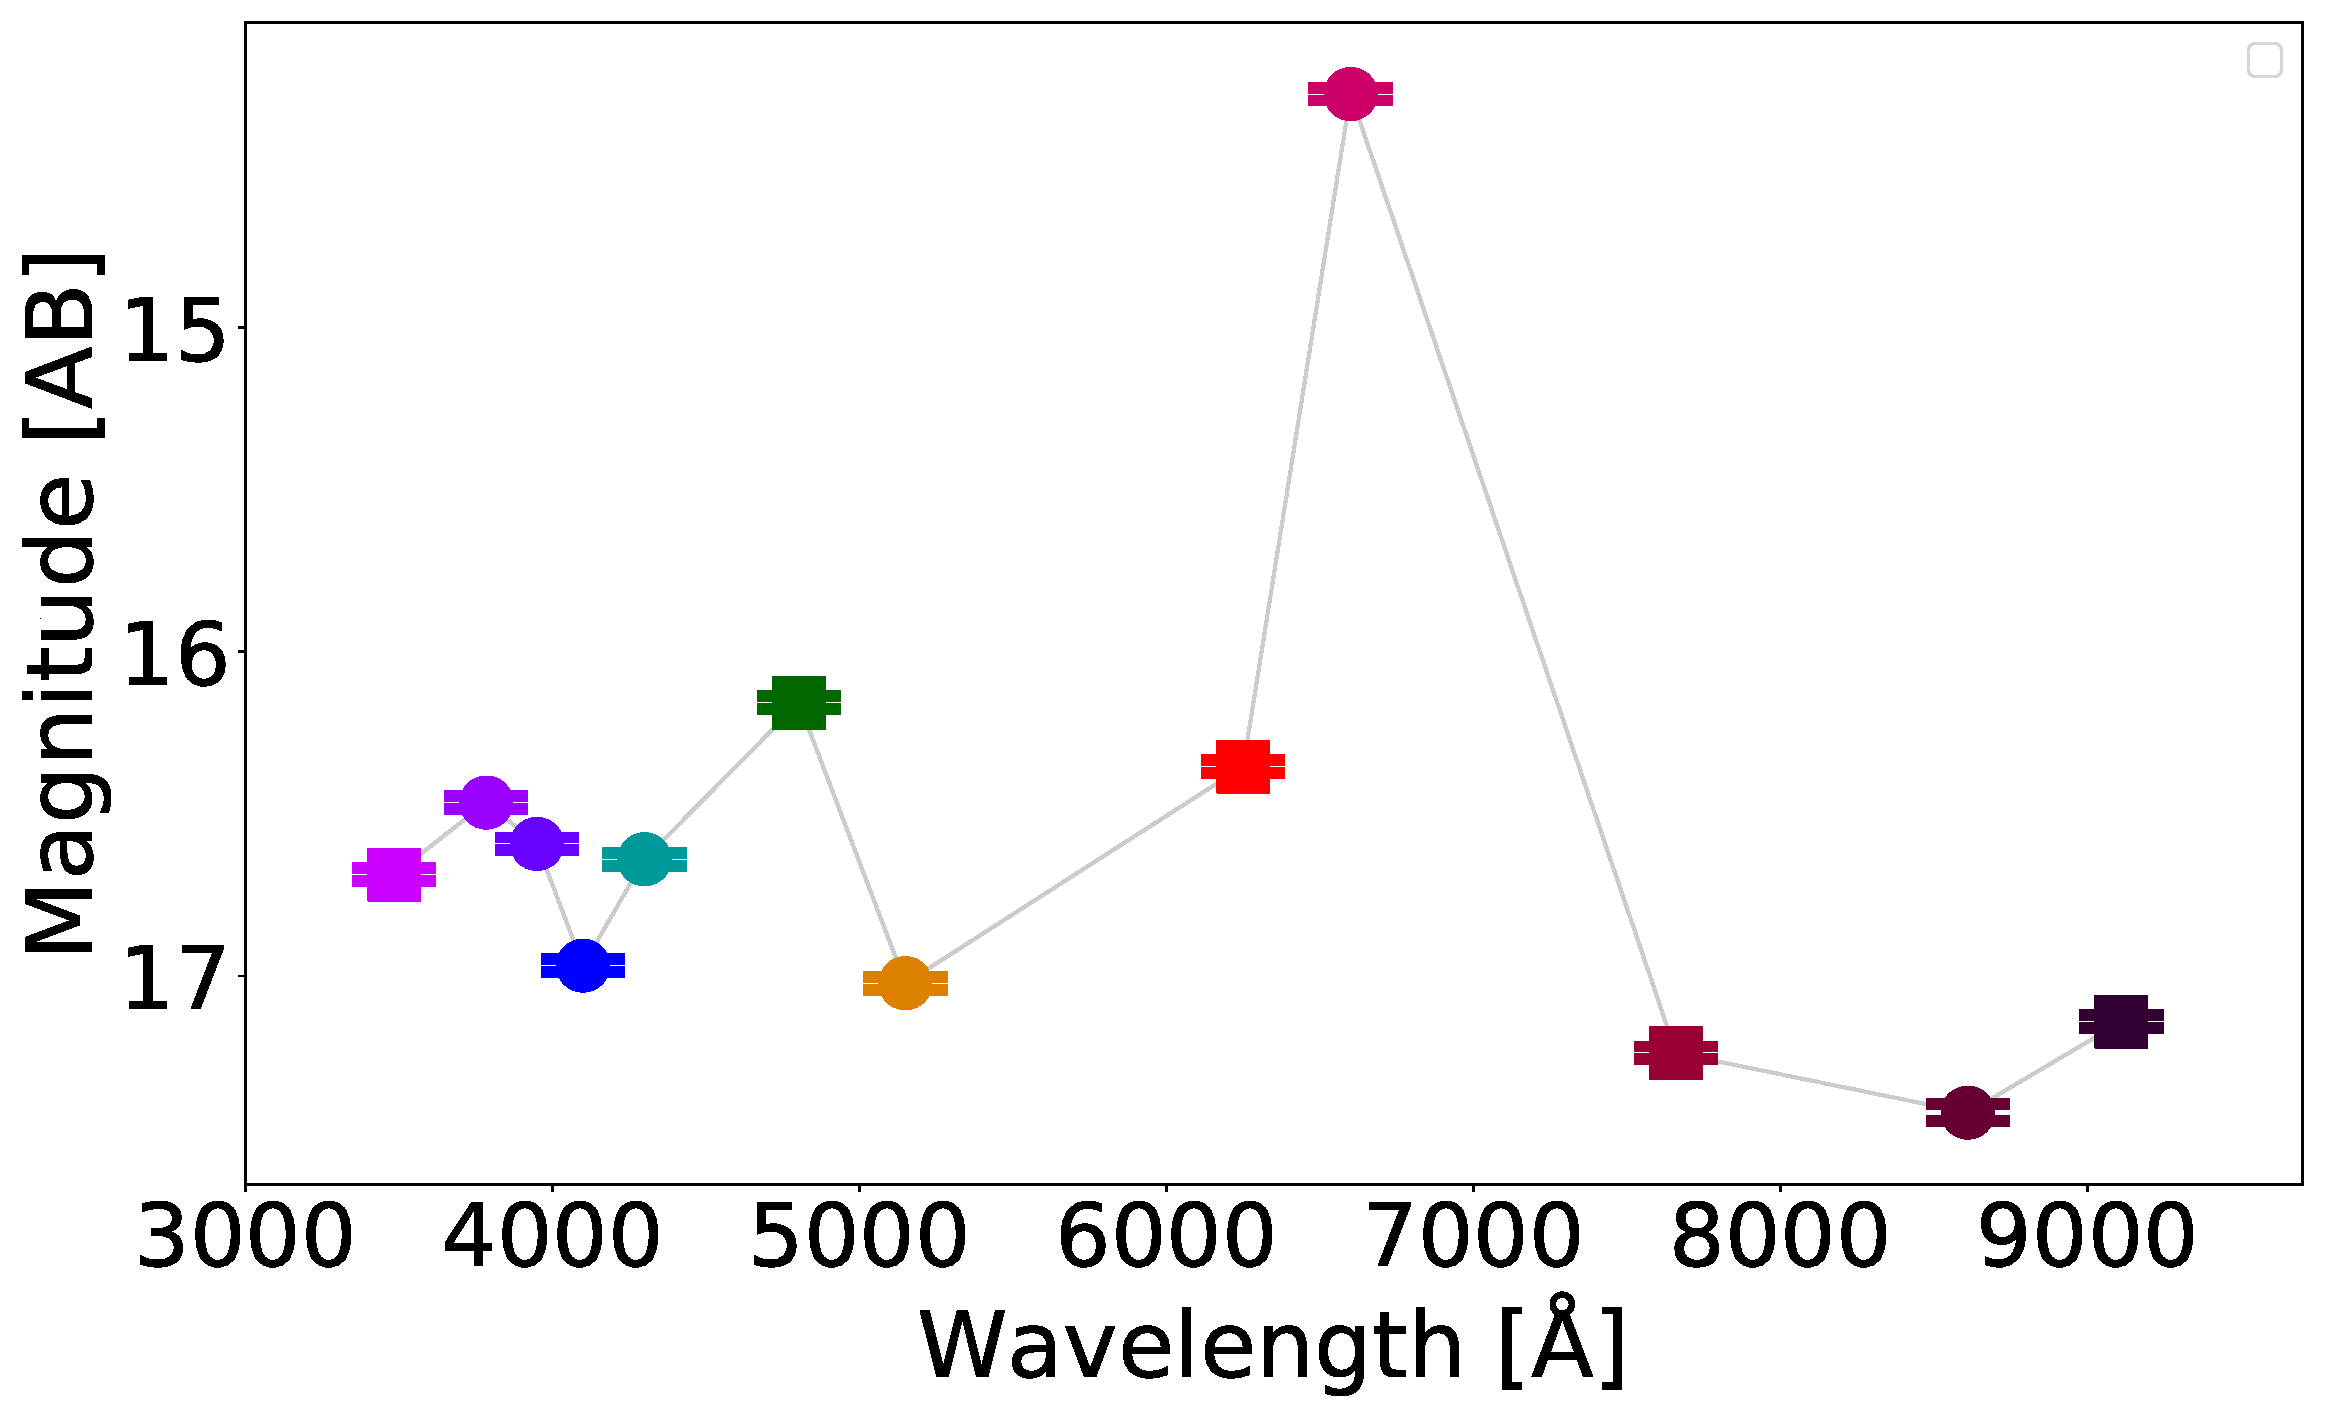
\includegraphics[width=0.3\linewidth, clip]{photopectrum_splus_MC0094-194143_petro.pdf} \\
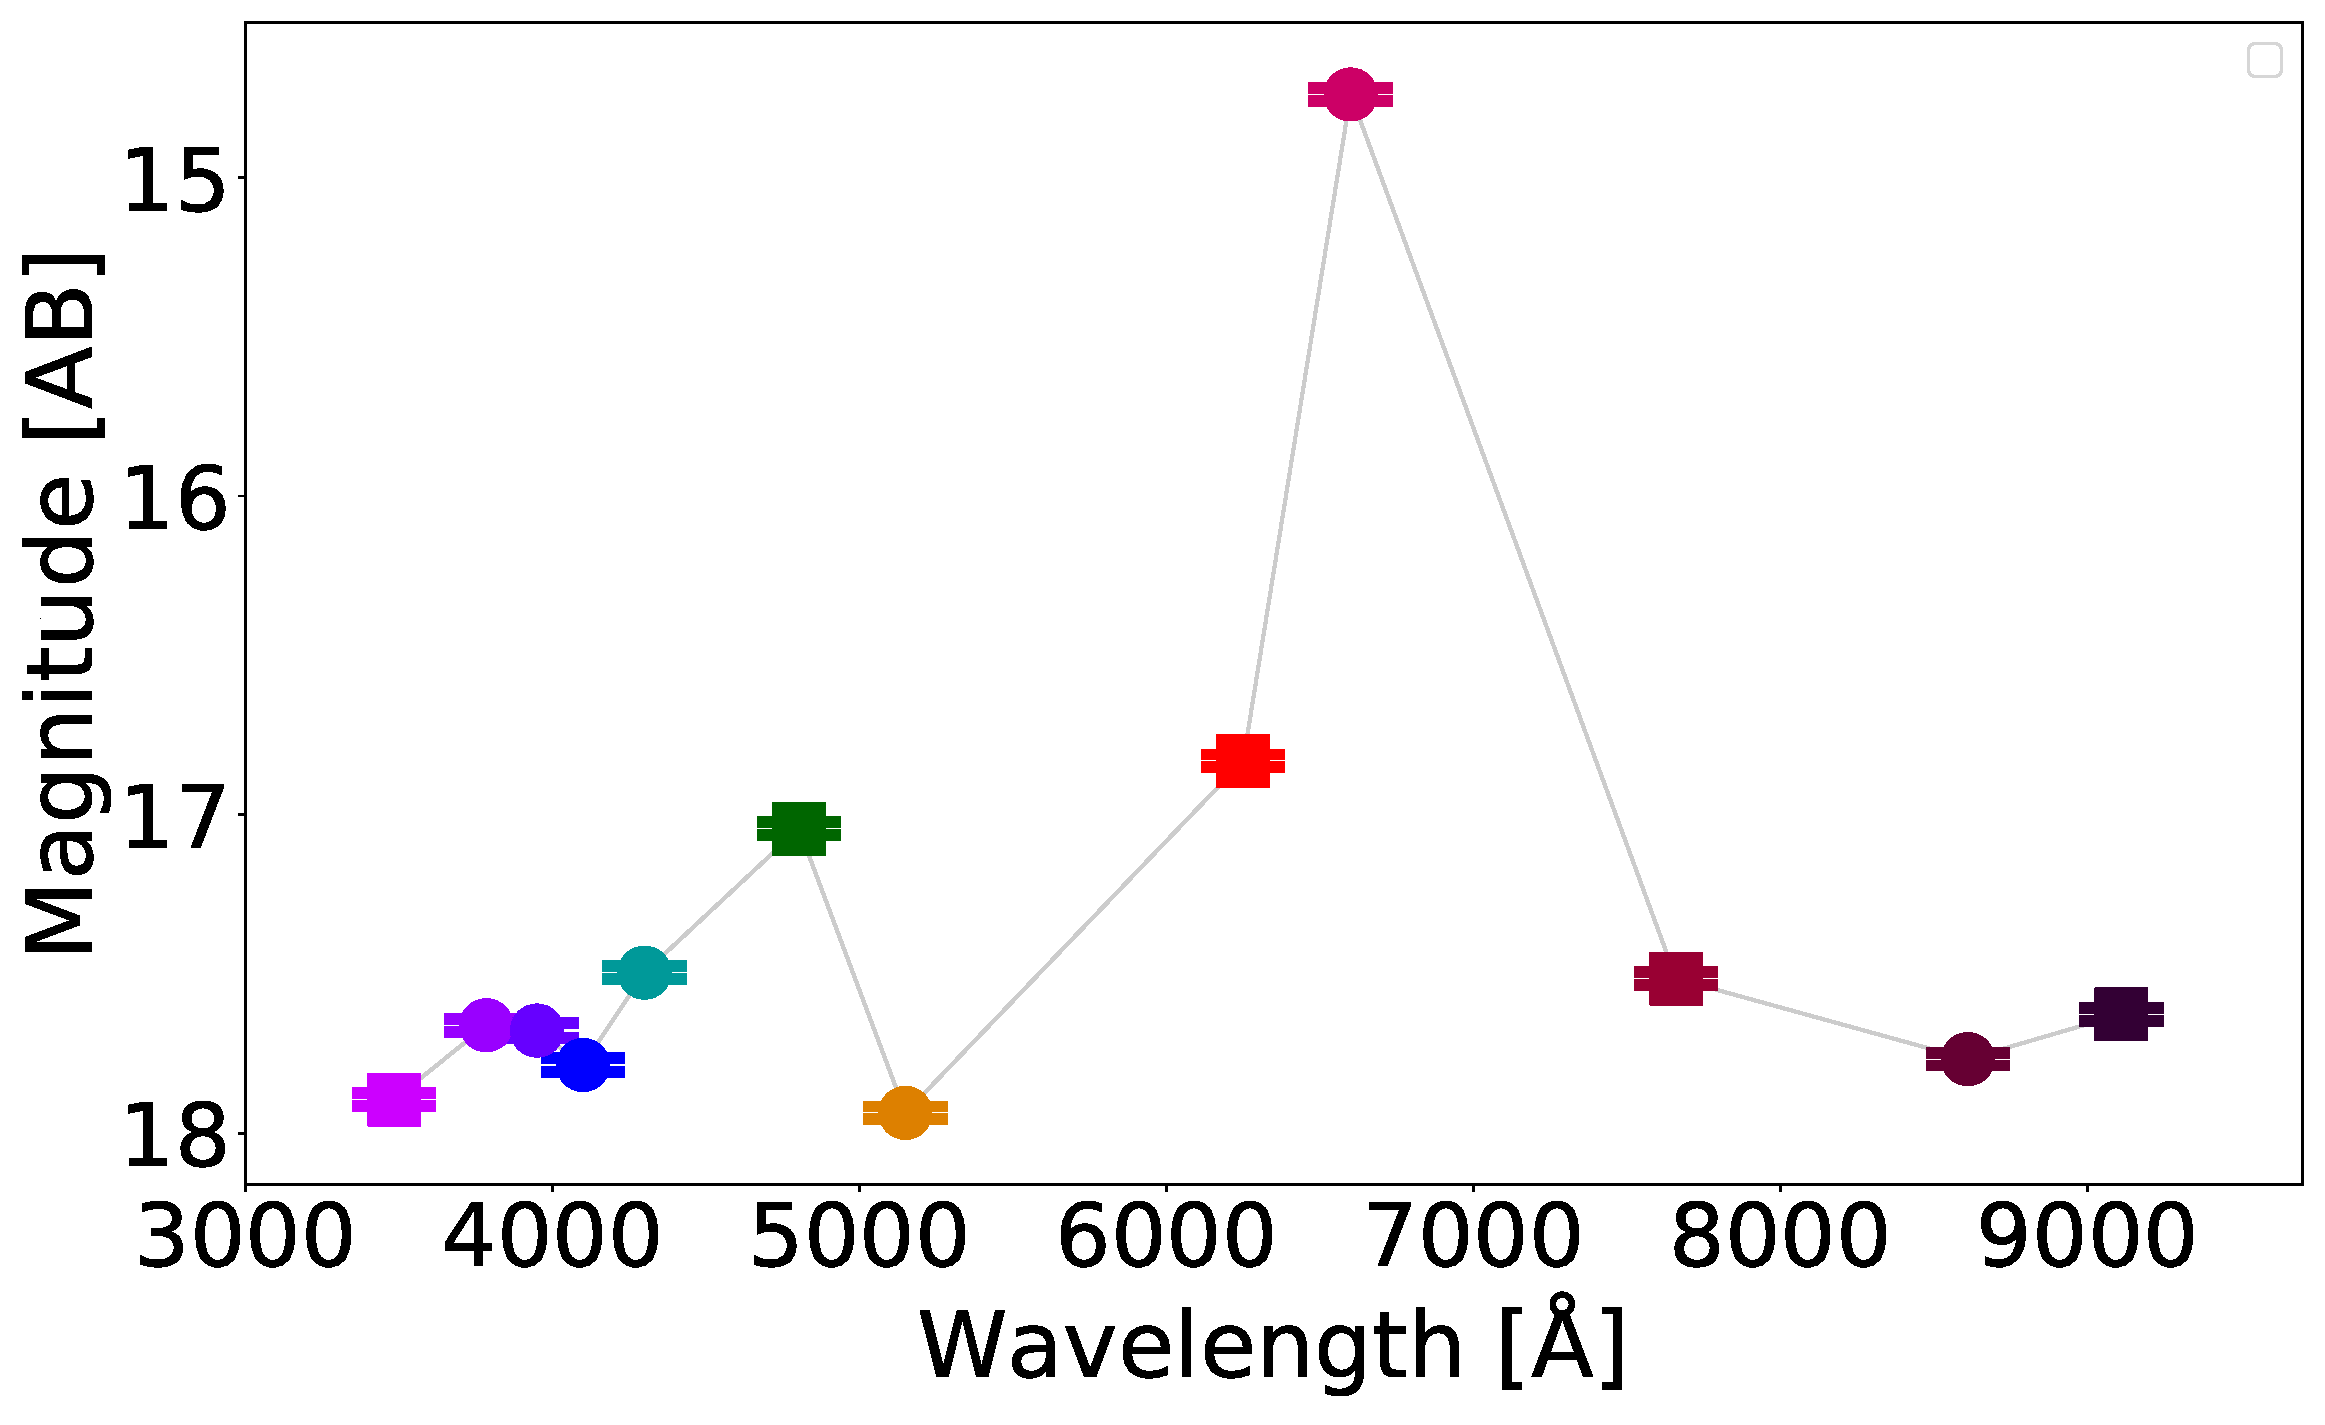
\includegraphics[width=0.3\linewidth, clip]{photopectrum_splus_MC0113-084466_aper.pdf} & 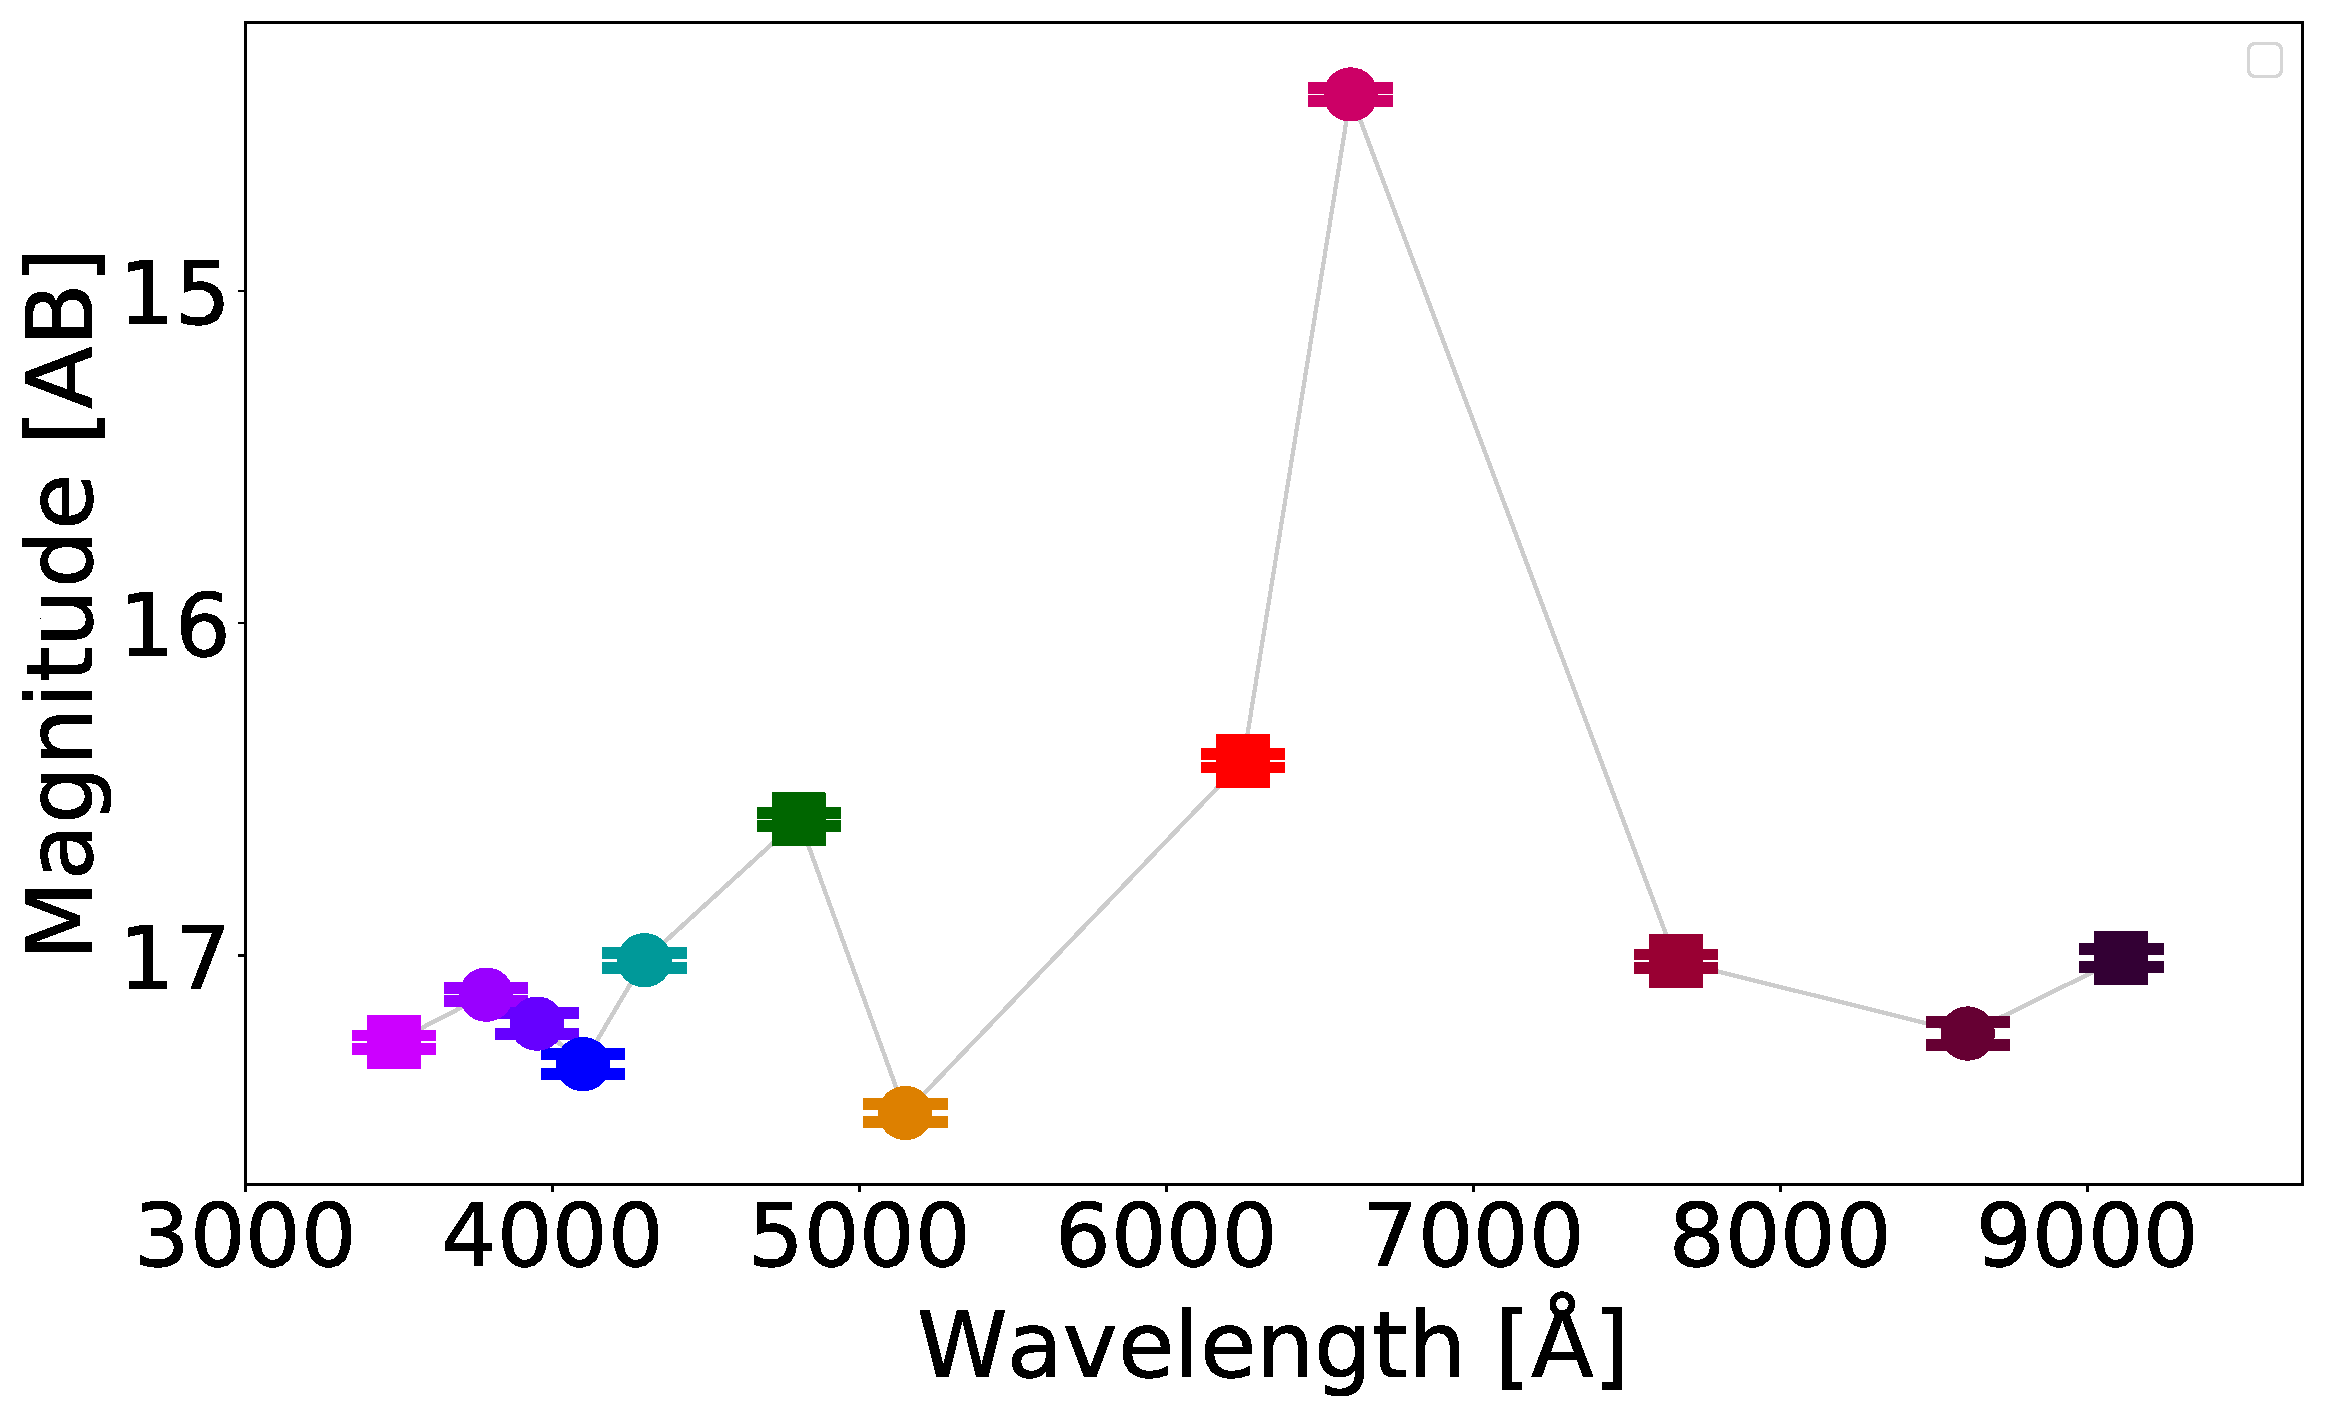
\includegraphics[width=0.3\linewidth, clip]{photopectrum_splus_MC0113-084466_auto.pdf} & 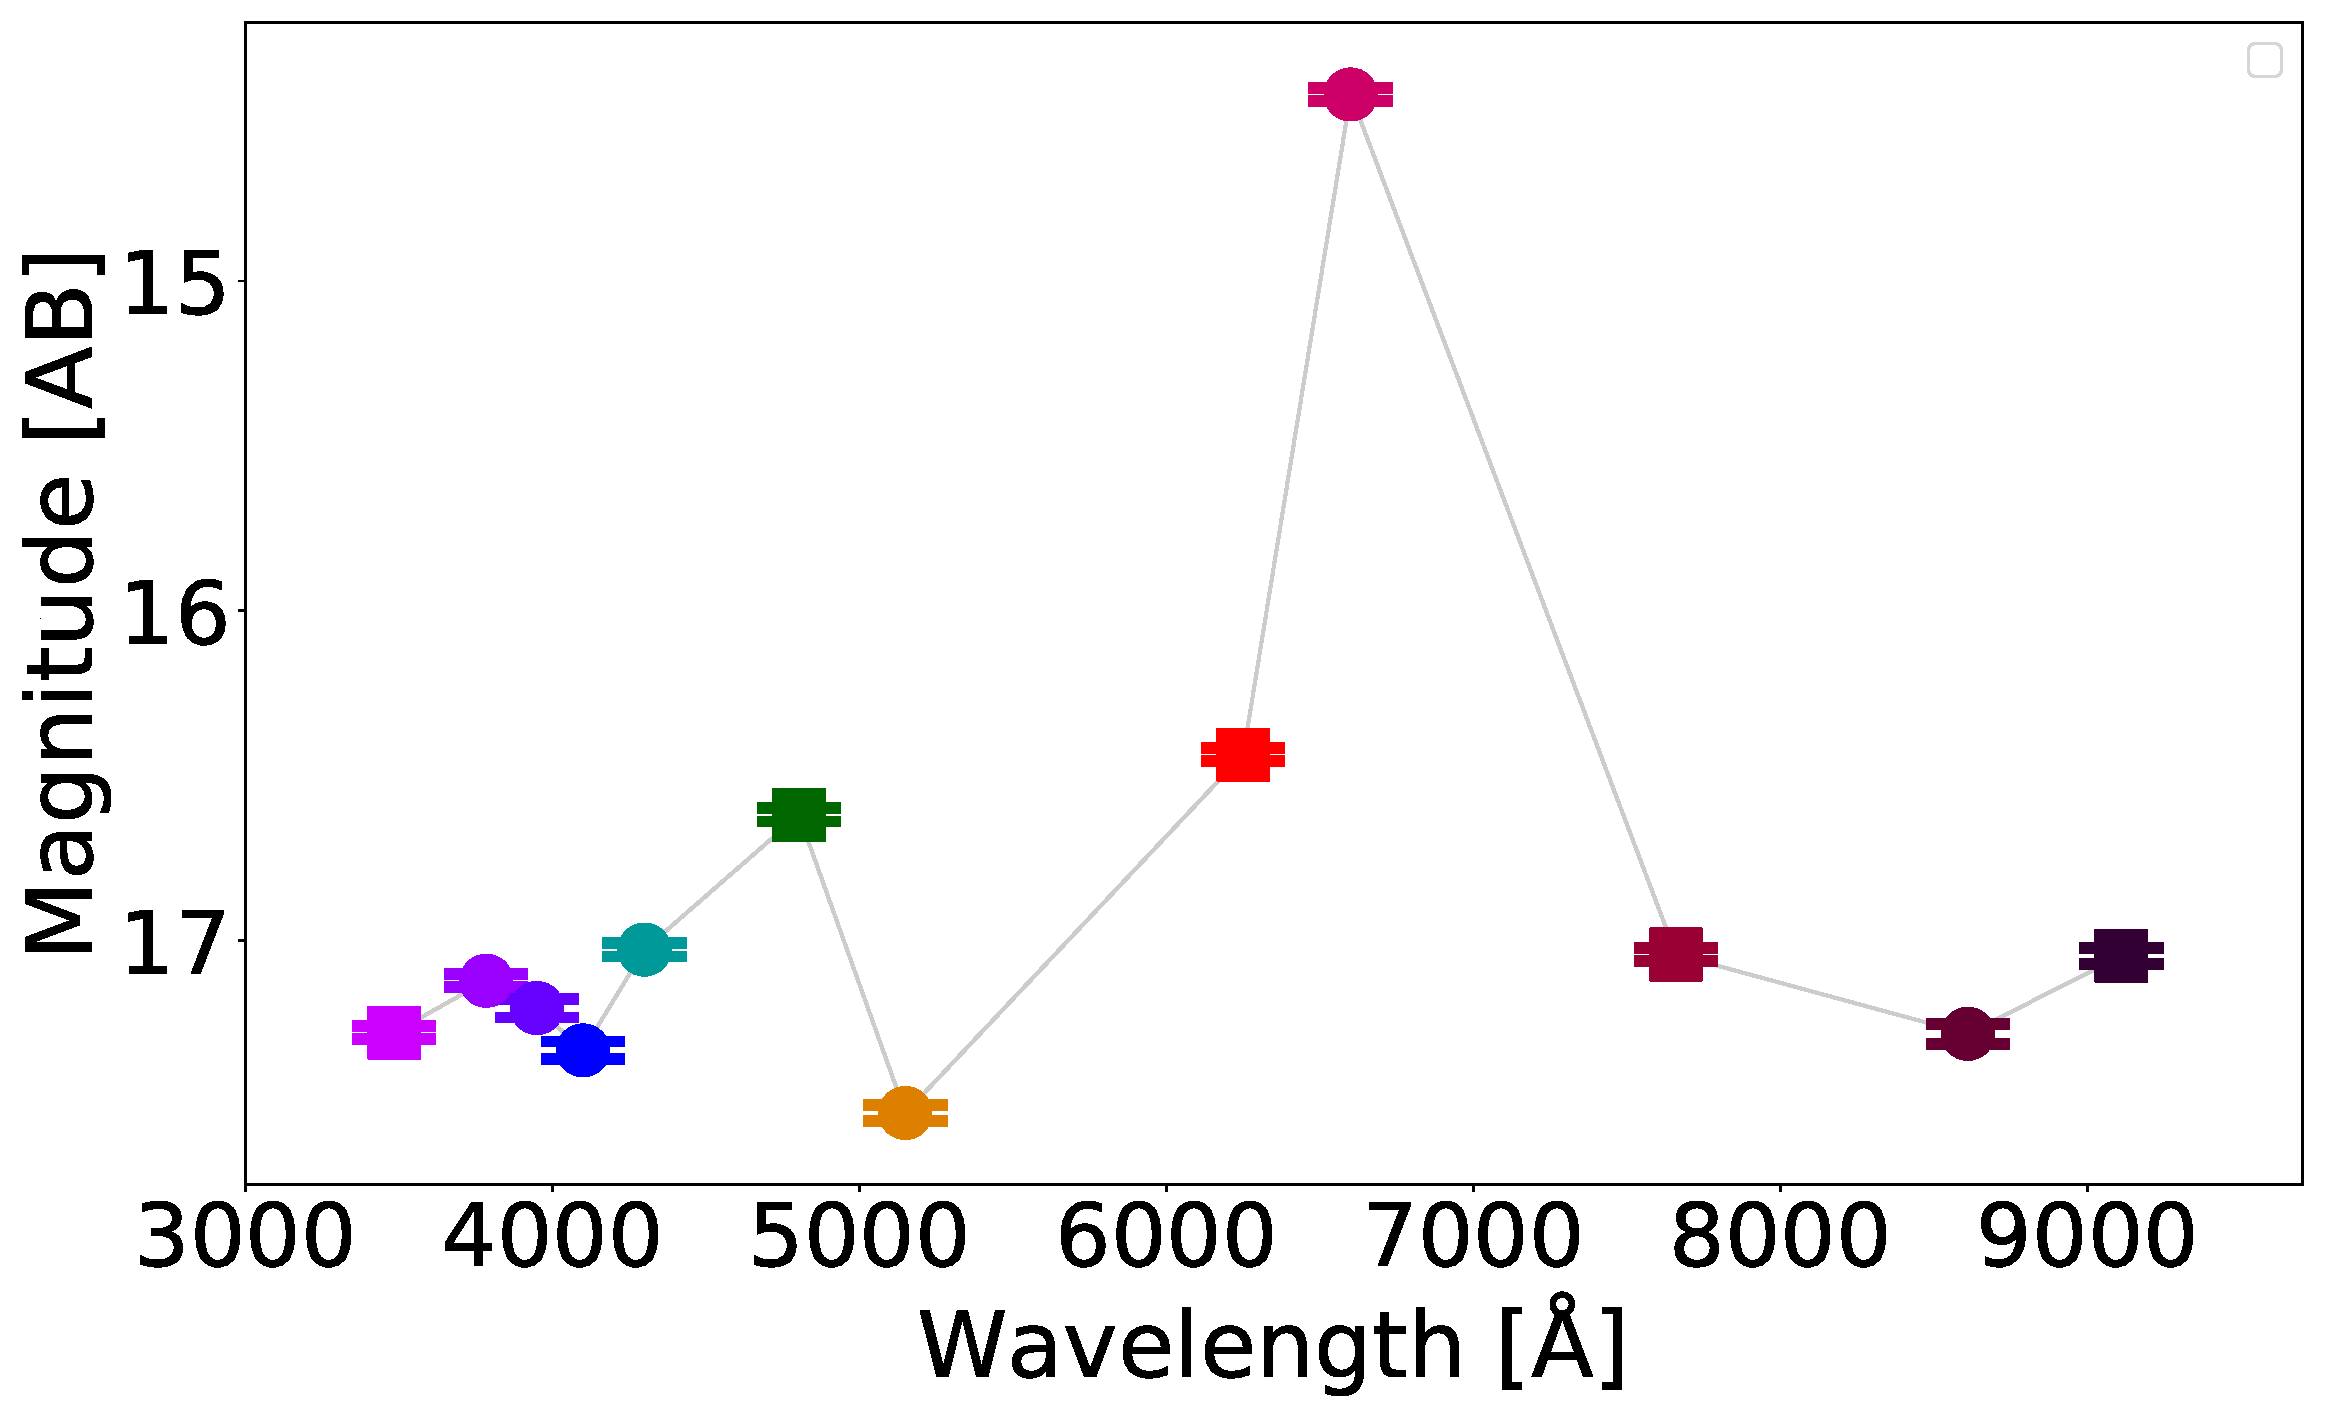
\includegraphics[width=0.3\linewidth, clip]{photopectrum_splus_MC0113-084466_petro.pdf} \\
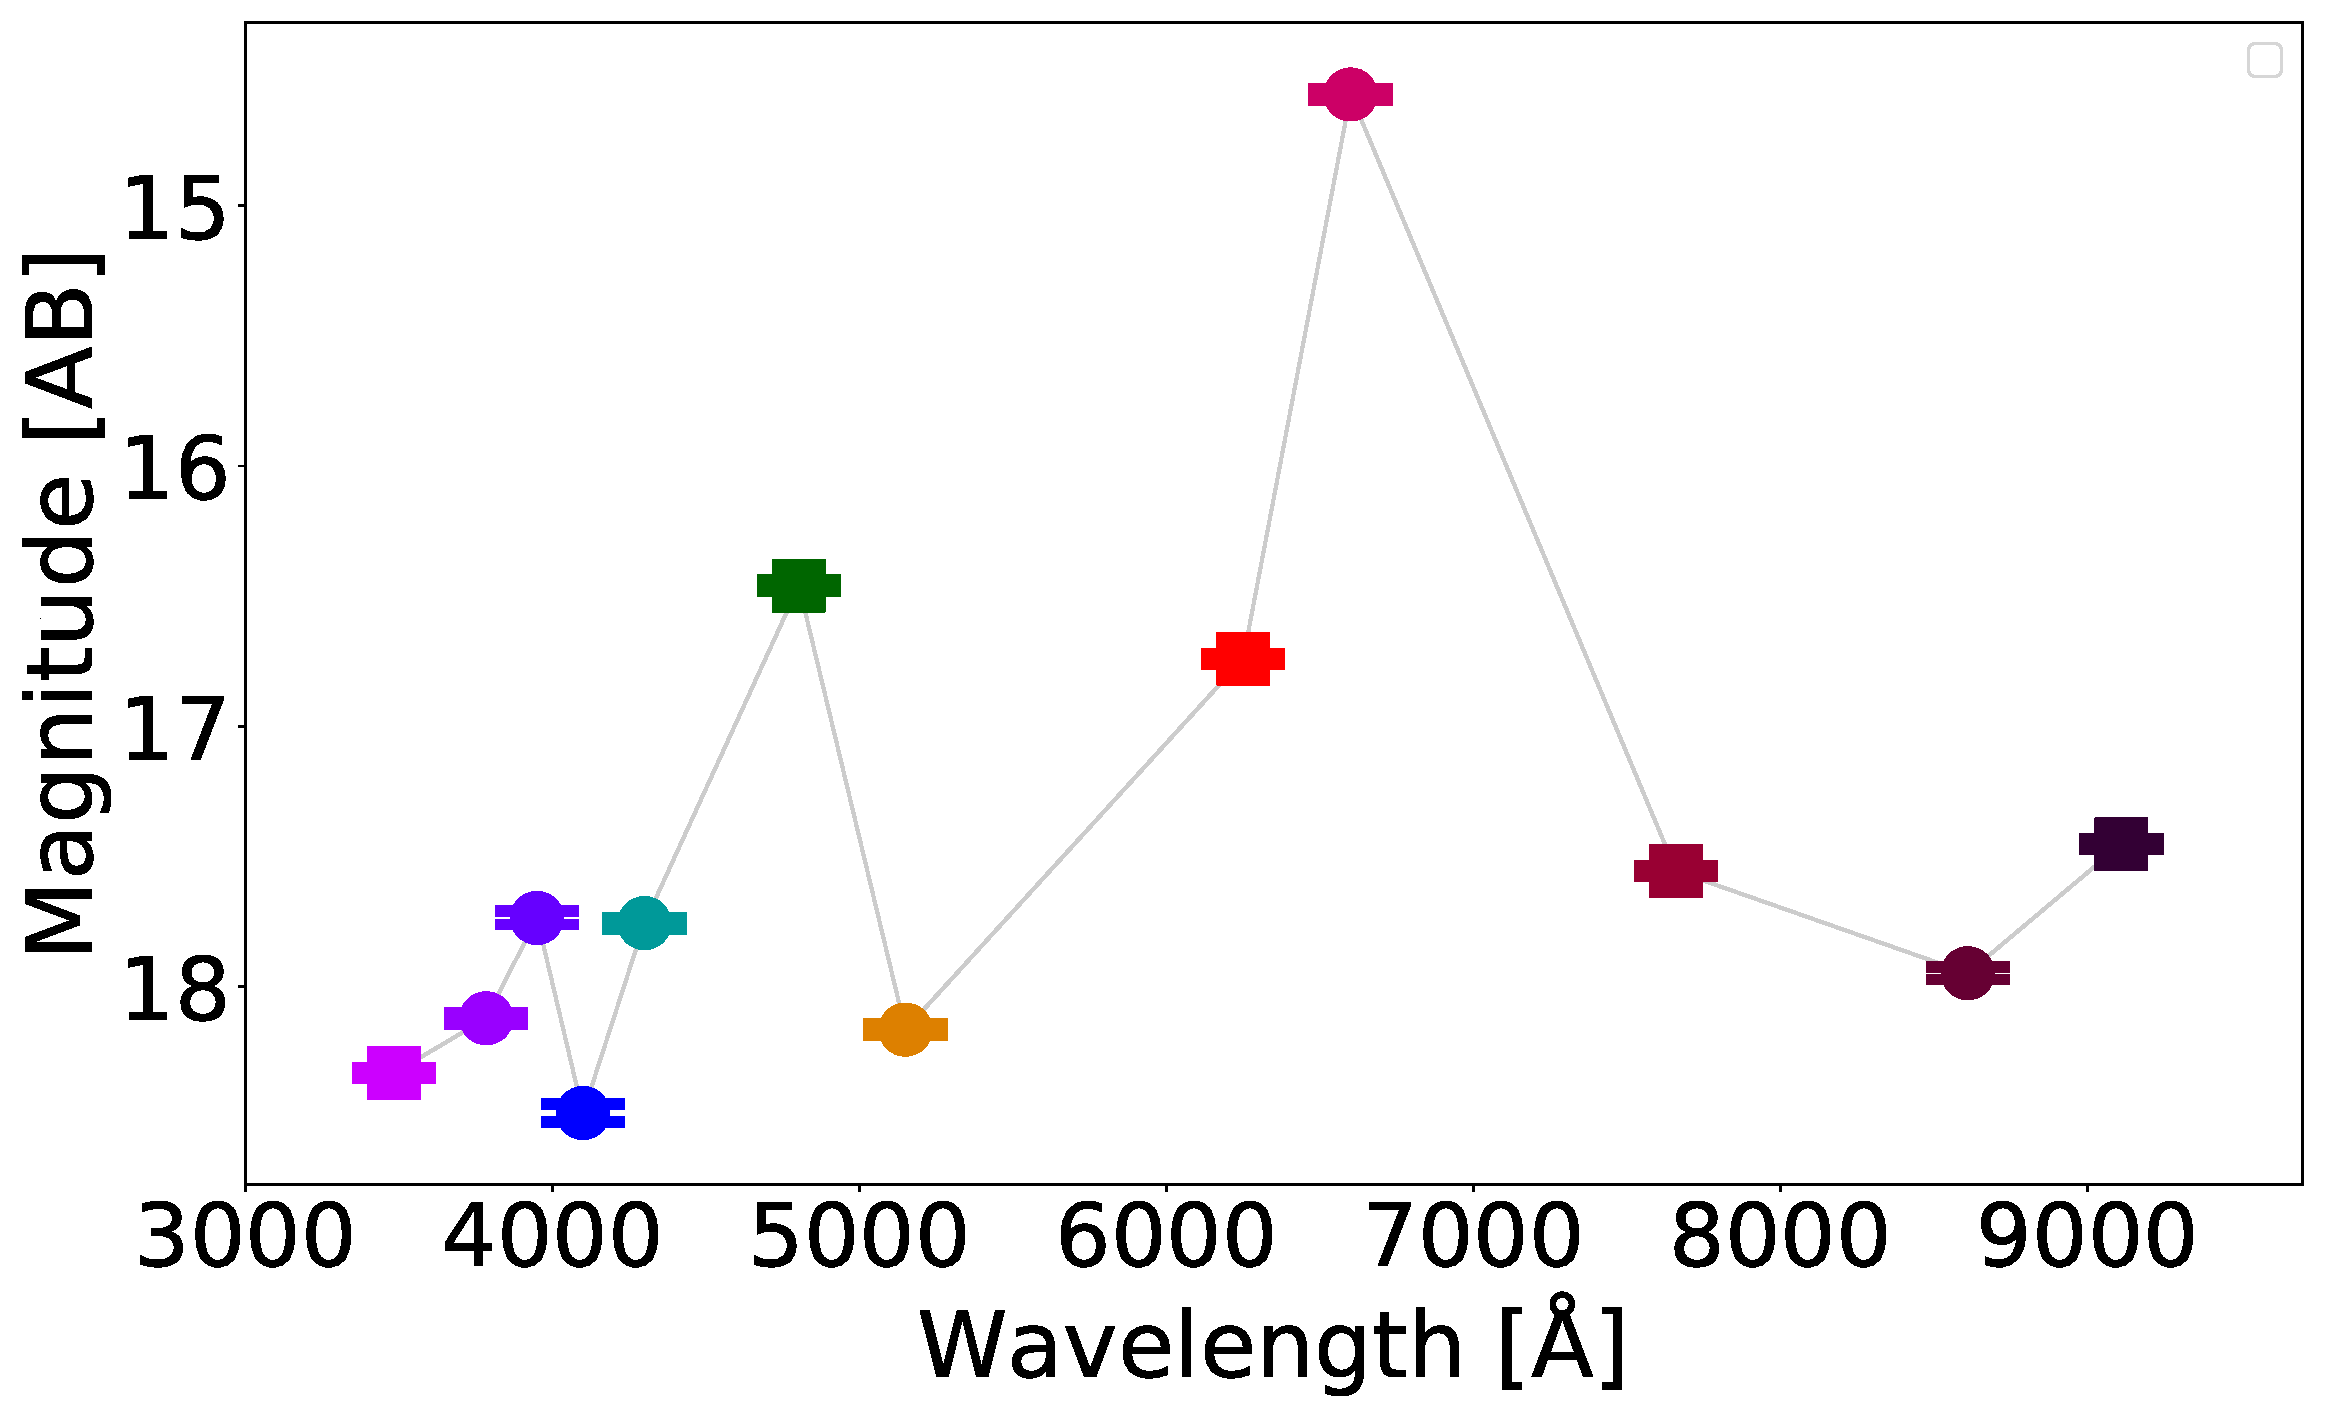
\includegraphics[width=0.3\linewidth, clip]{photopectrum_splus_MC0114-113862_aper.pdf} & 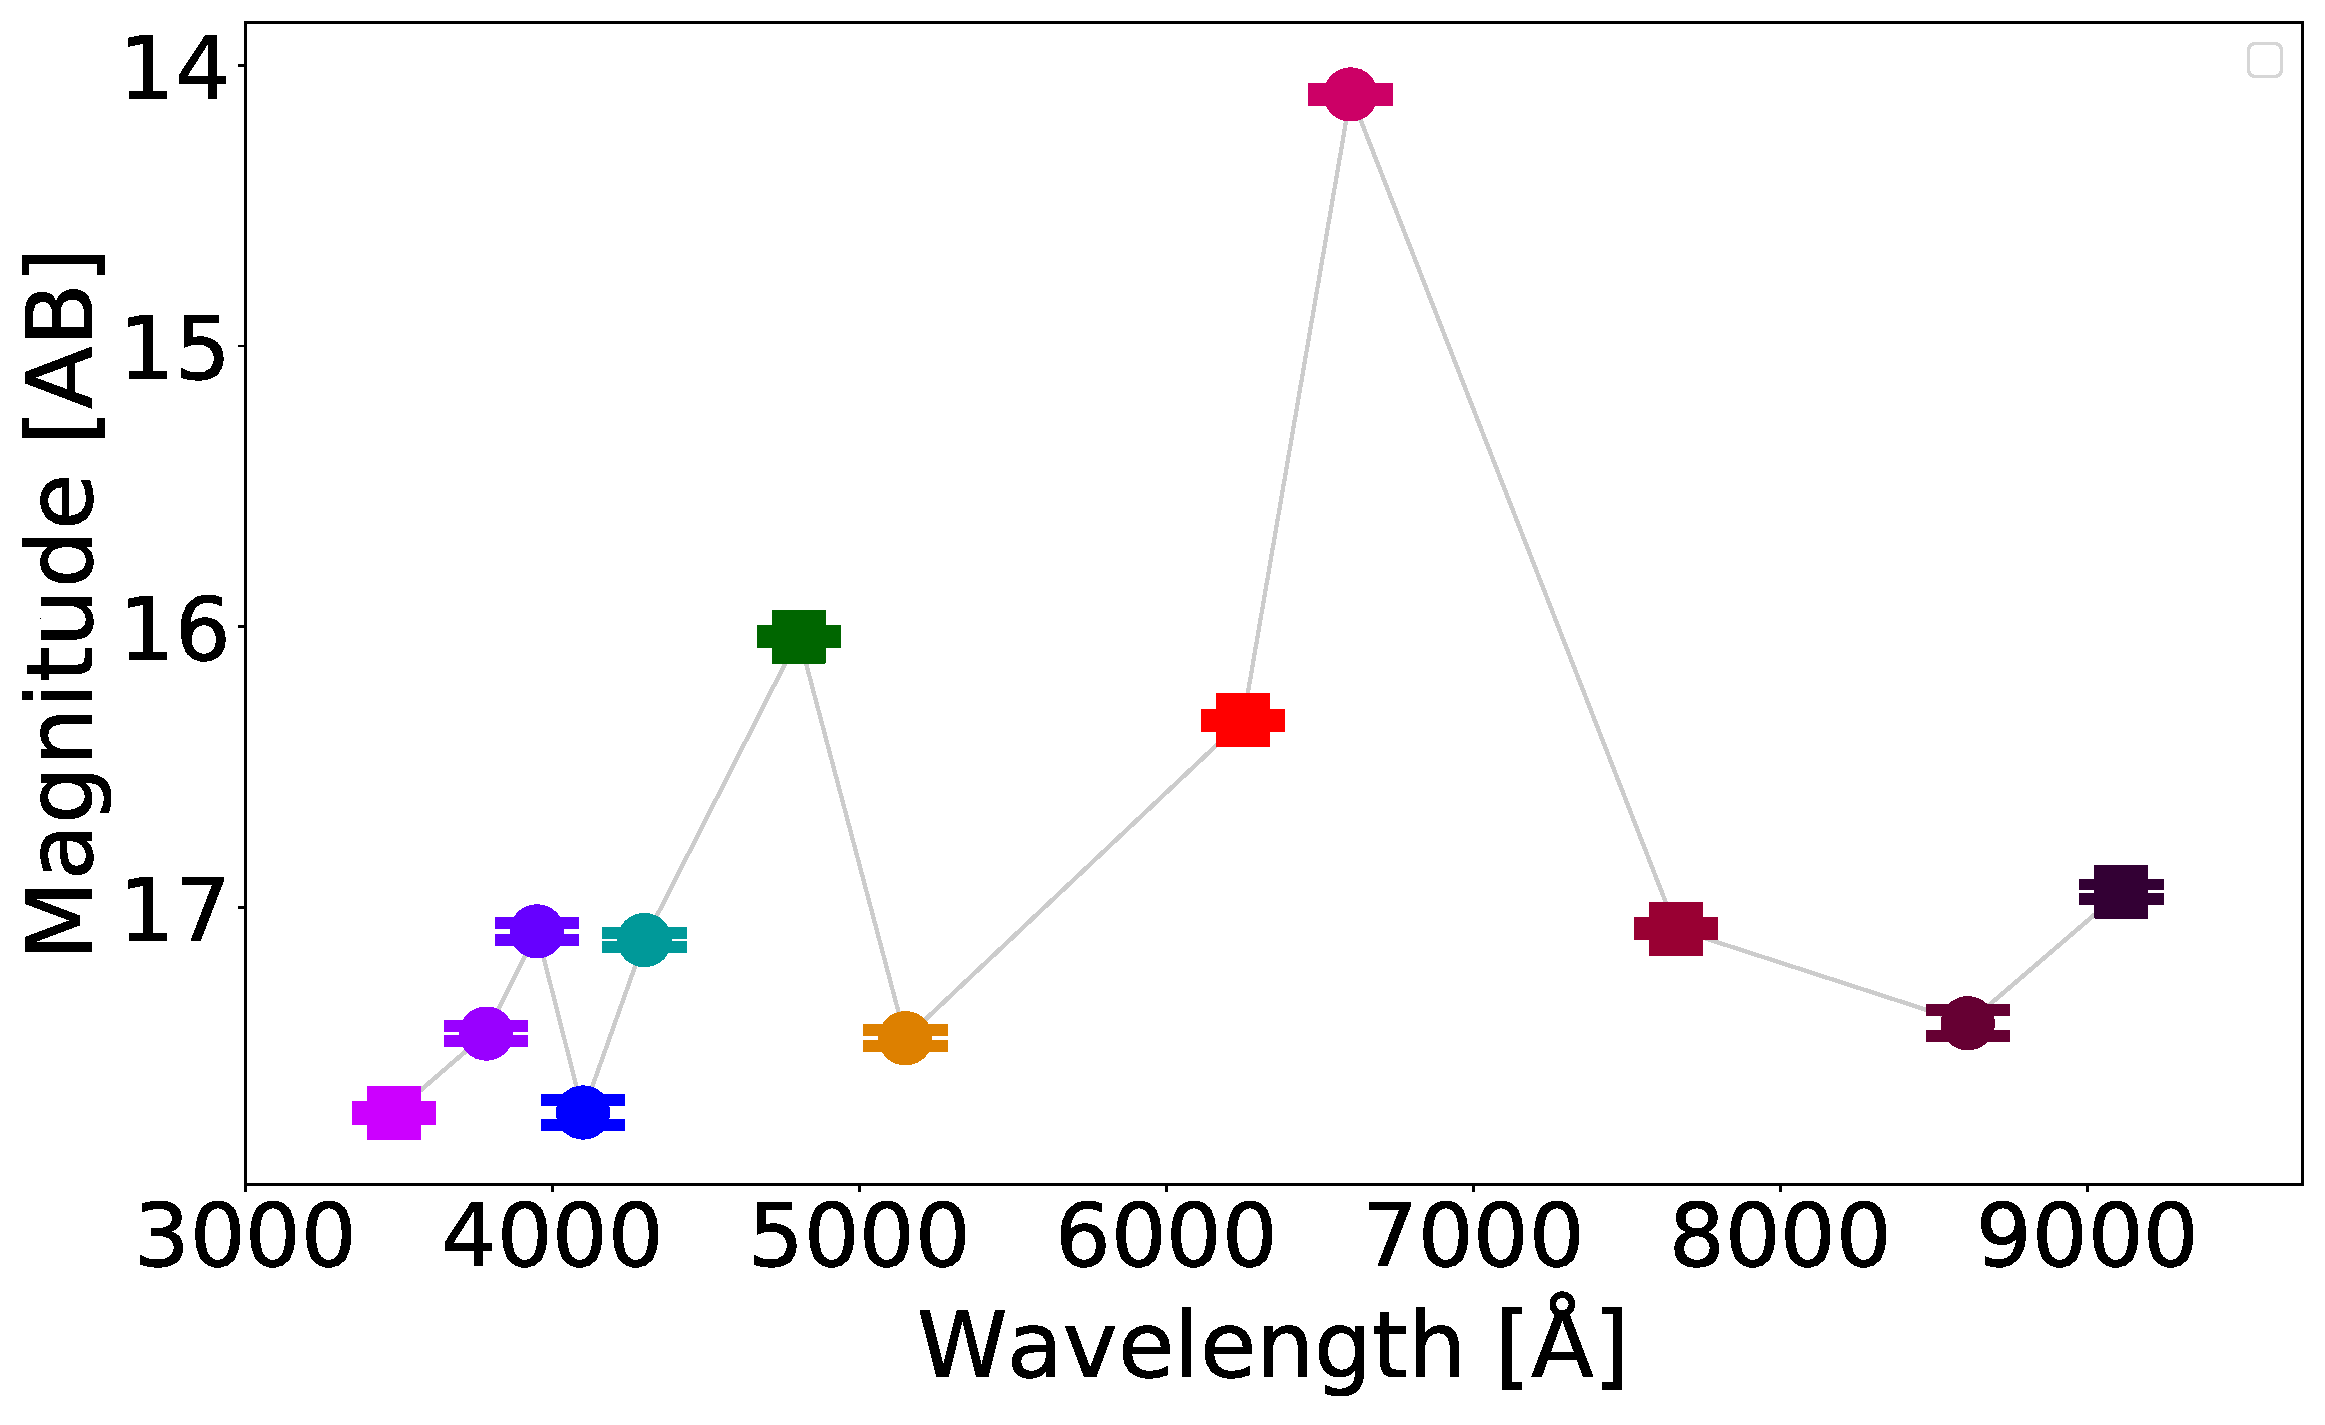
\includegraphics[width=0.3\linewidth, clip]{photopectrum_splus_MC0114-113862_auto.pdf} & 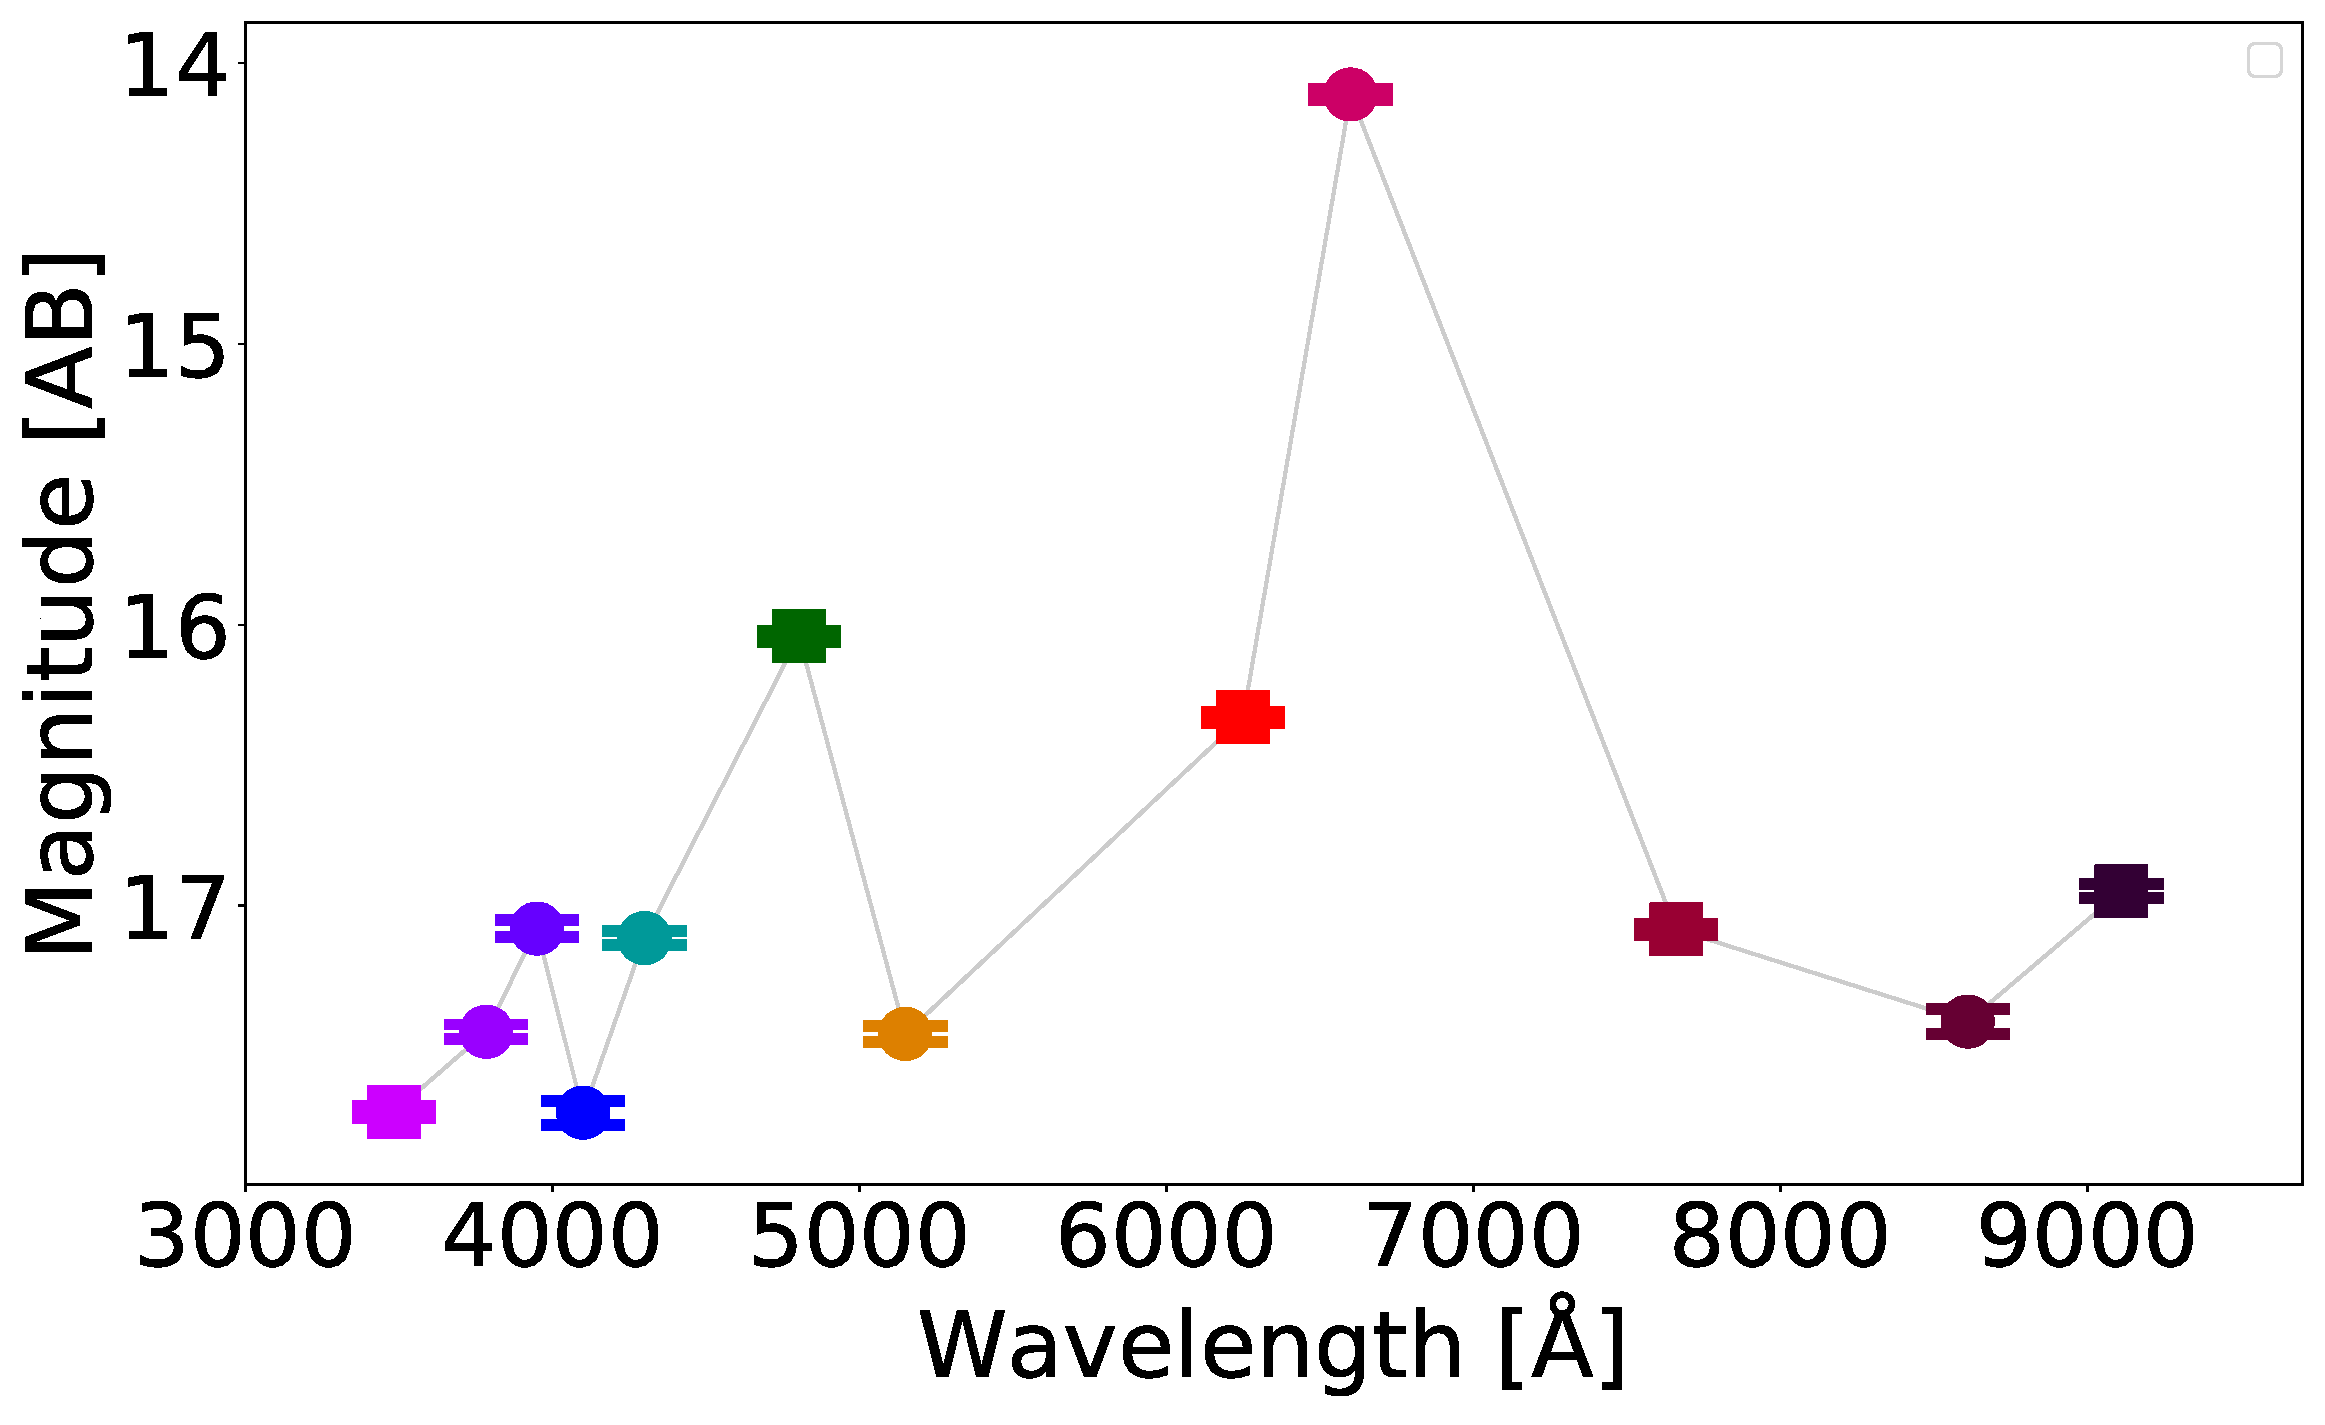
\includegraphics[width=0.3\linewidth, clip]{photopectrum_splus_MC0114-113862_petro.pdf} \\

\end{tabular}
\end{table}

\begin{table}
\begin{tabular}{ccc}

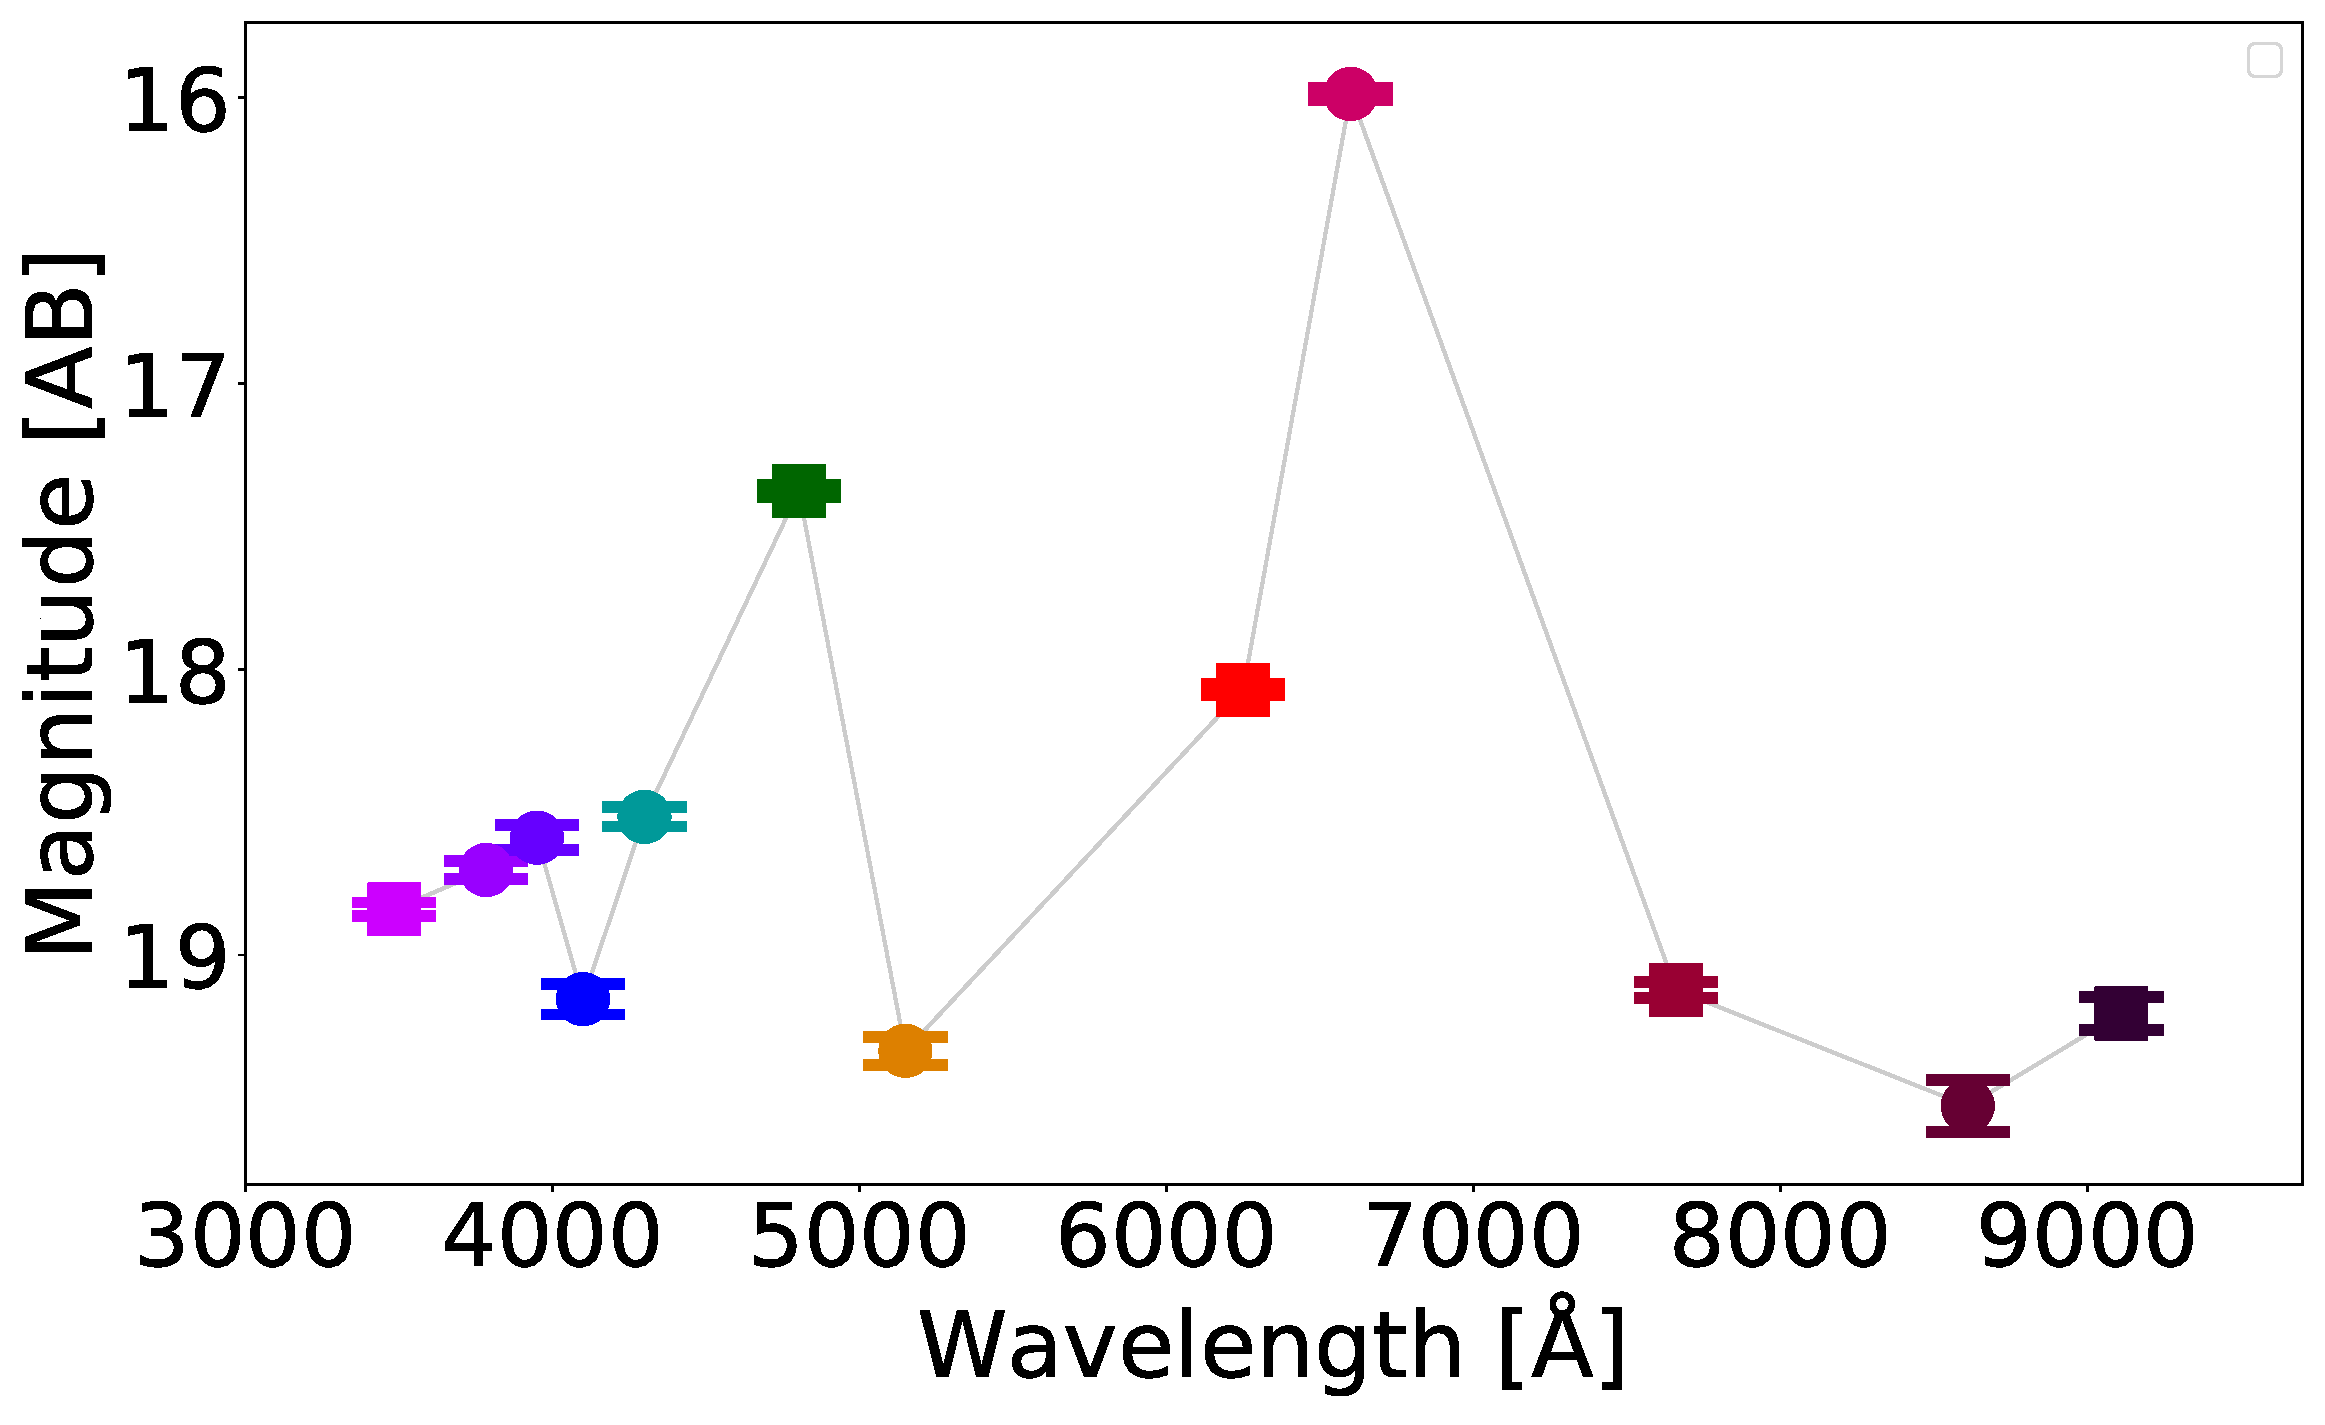
\includegraphics[width=0.3\linewidth, clip]{photopectrum_splus_MC0114-273678_aper.pdf} & 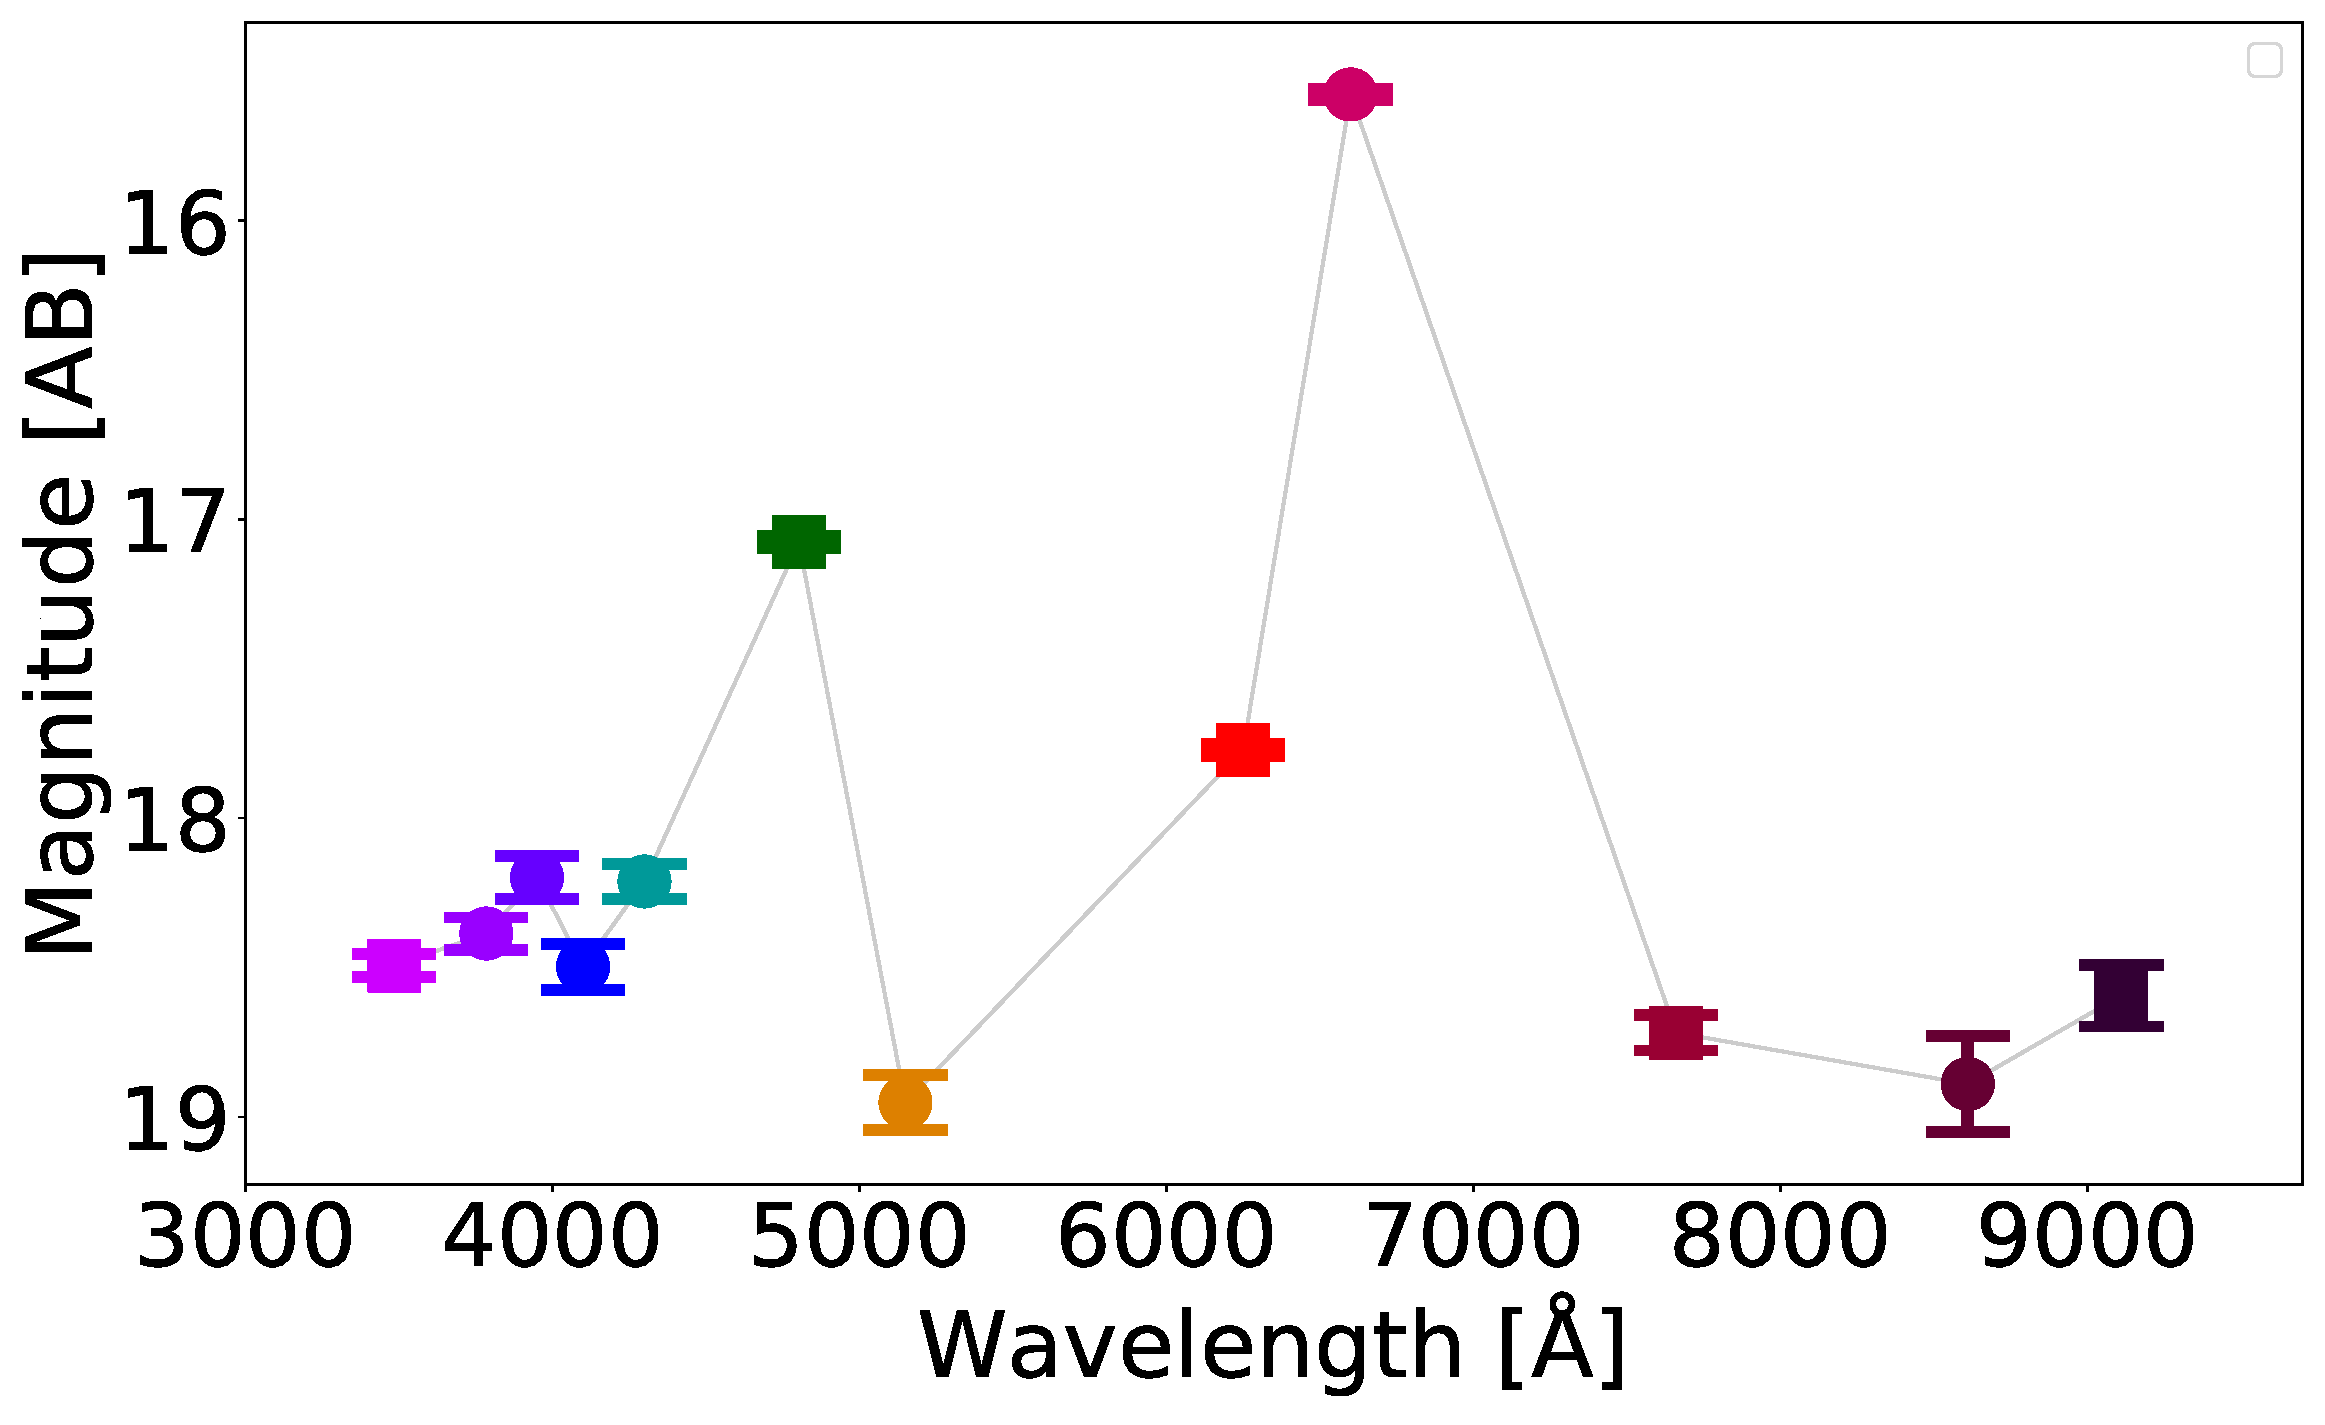
\includegraphics[width=0.3\linewidth, clip]{photopectrum_splus_MC0114-273678_auto.pdf} & 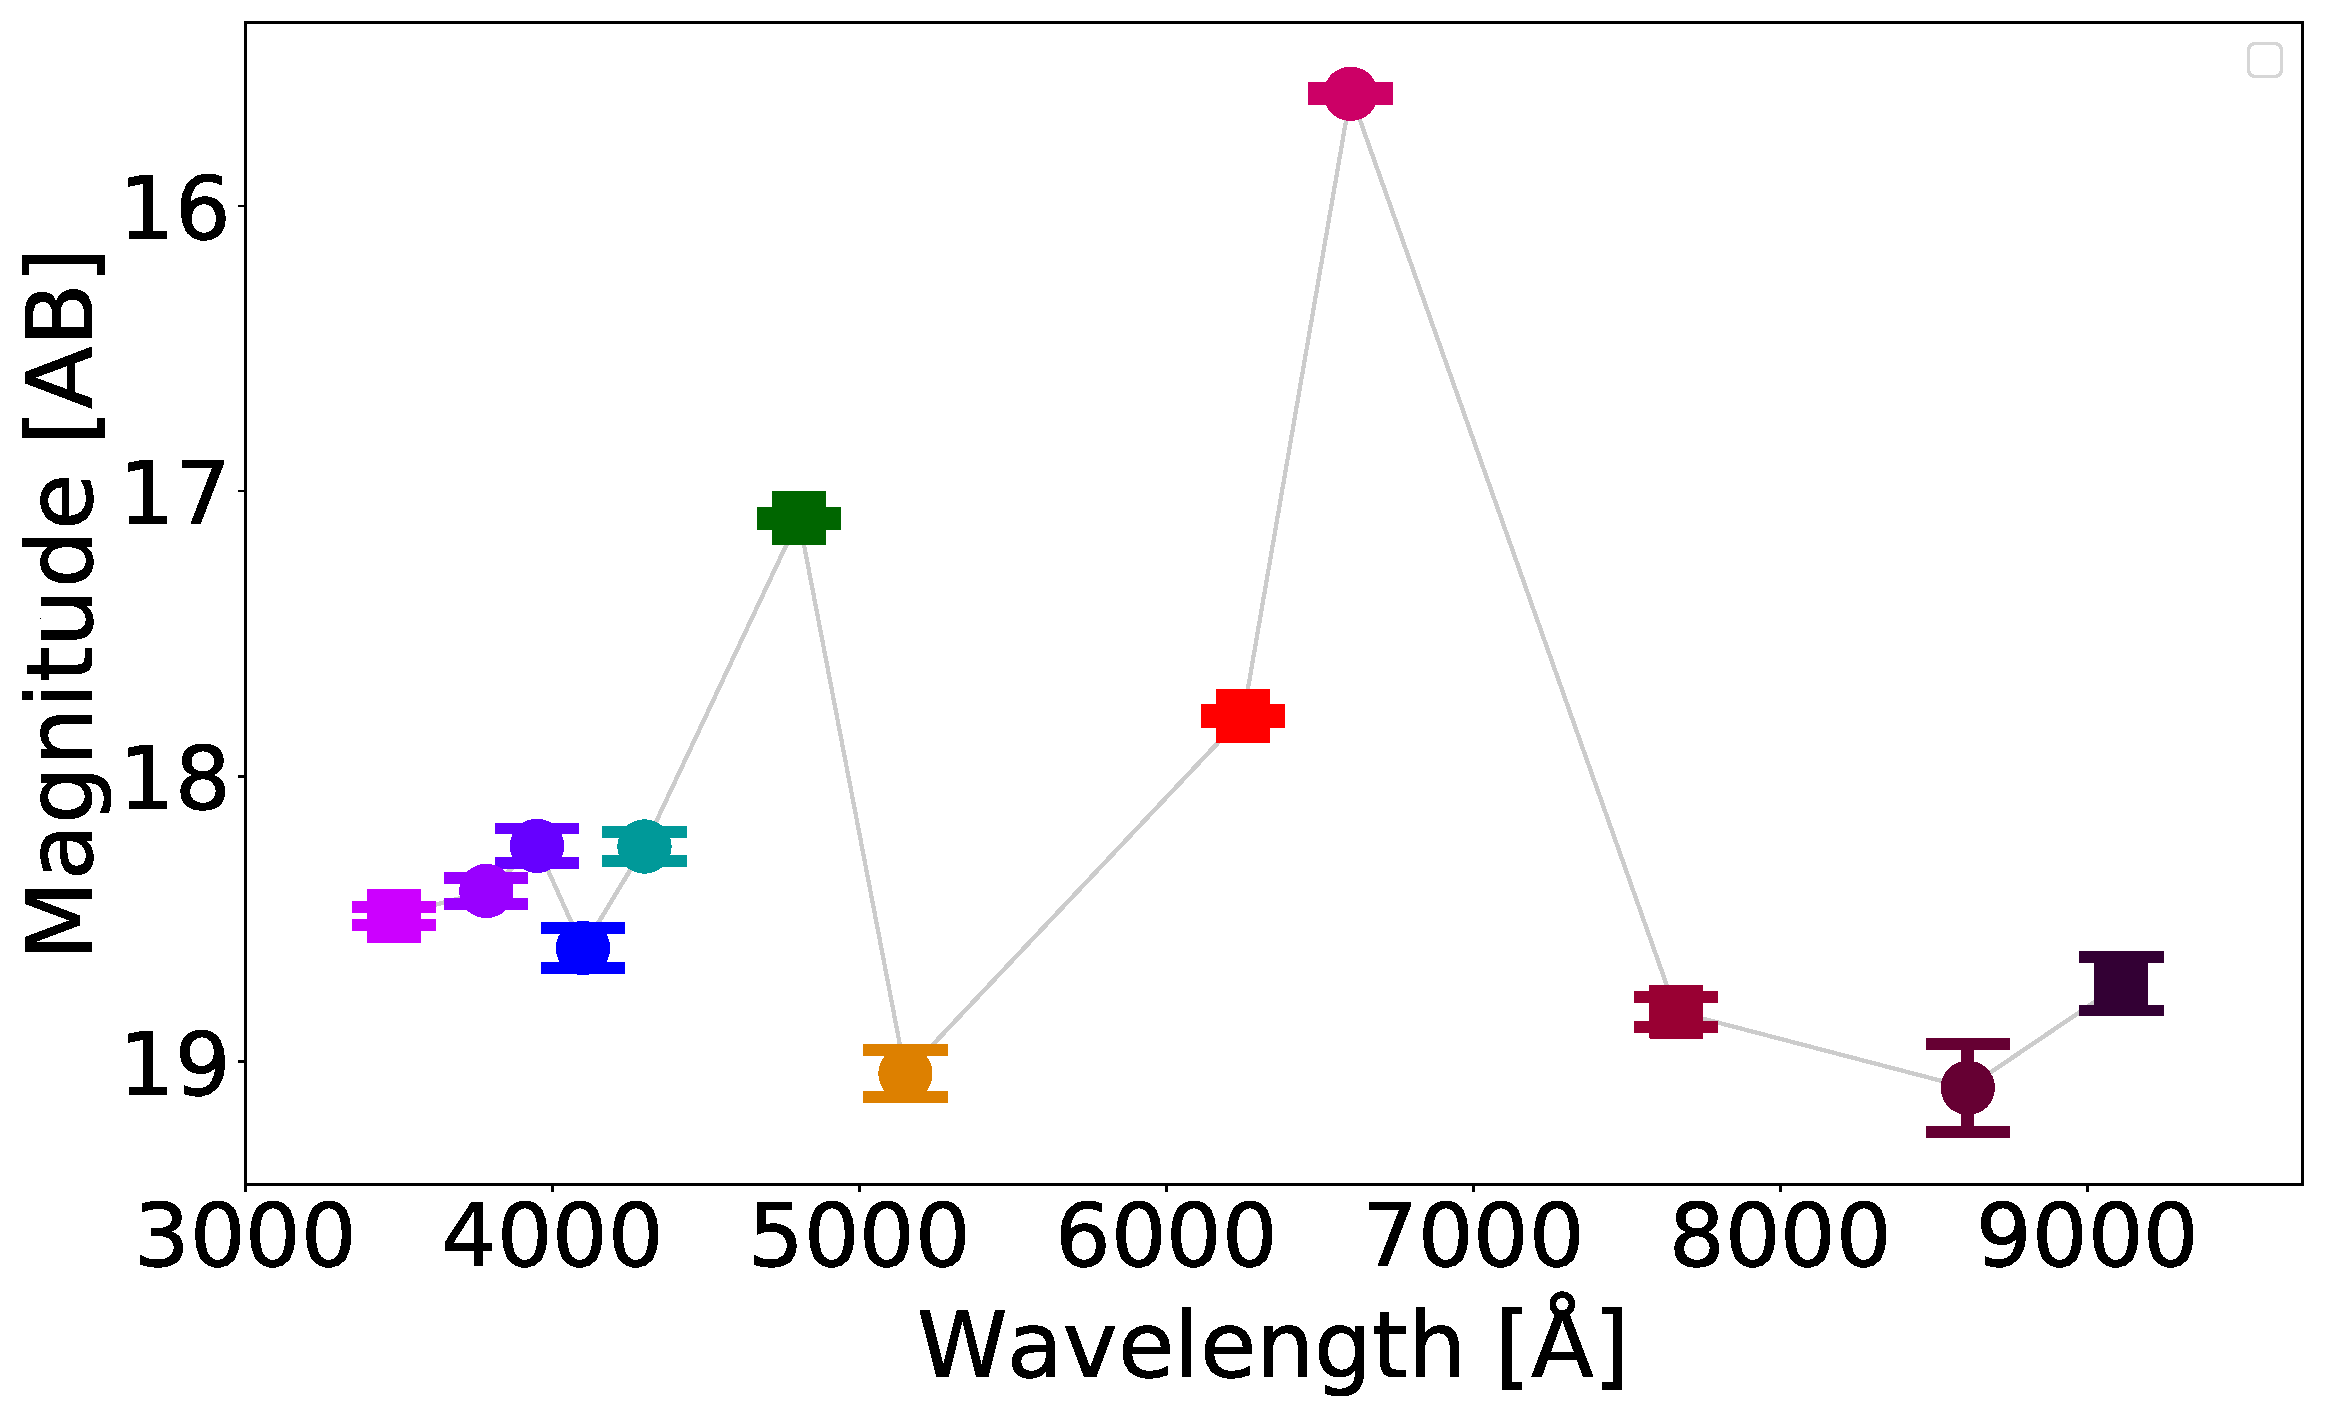
\includegraphics[width=0.3\linewidth, clip]{photopectrum_splus_MC0114-273678_petro.pdf} \\
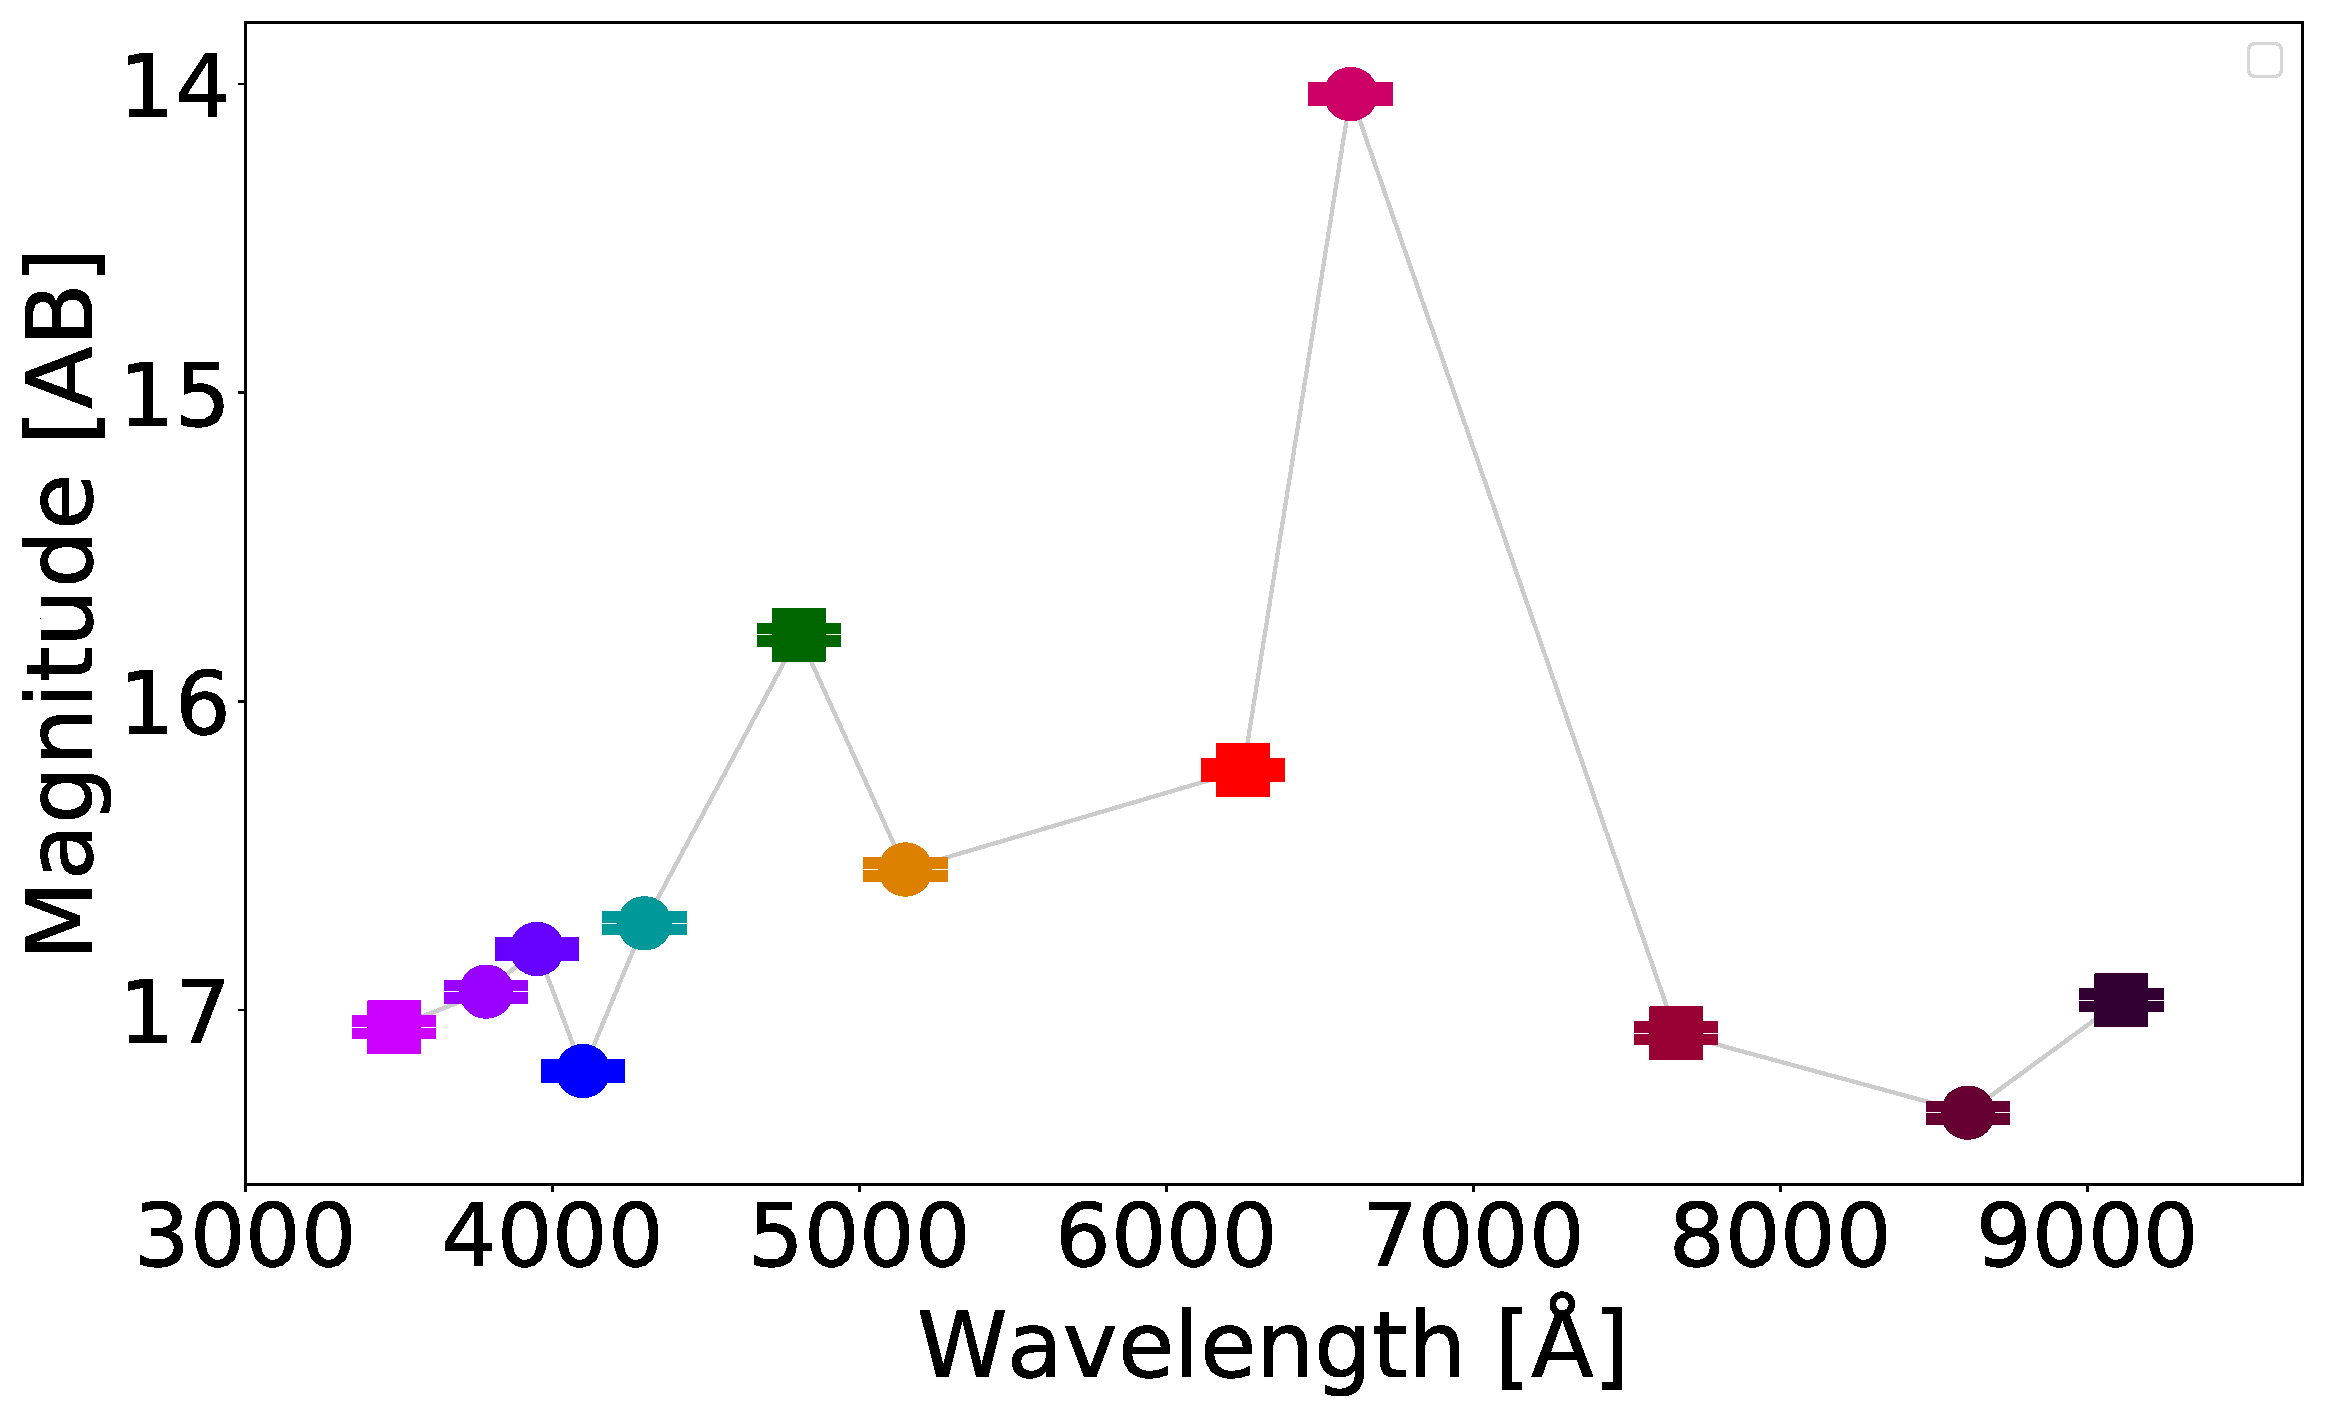
\includegraphics[width=0.3\linewidth, clip]{photopectrum_splus_MC0115-043944_aper.pdf} & 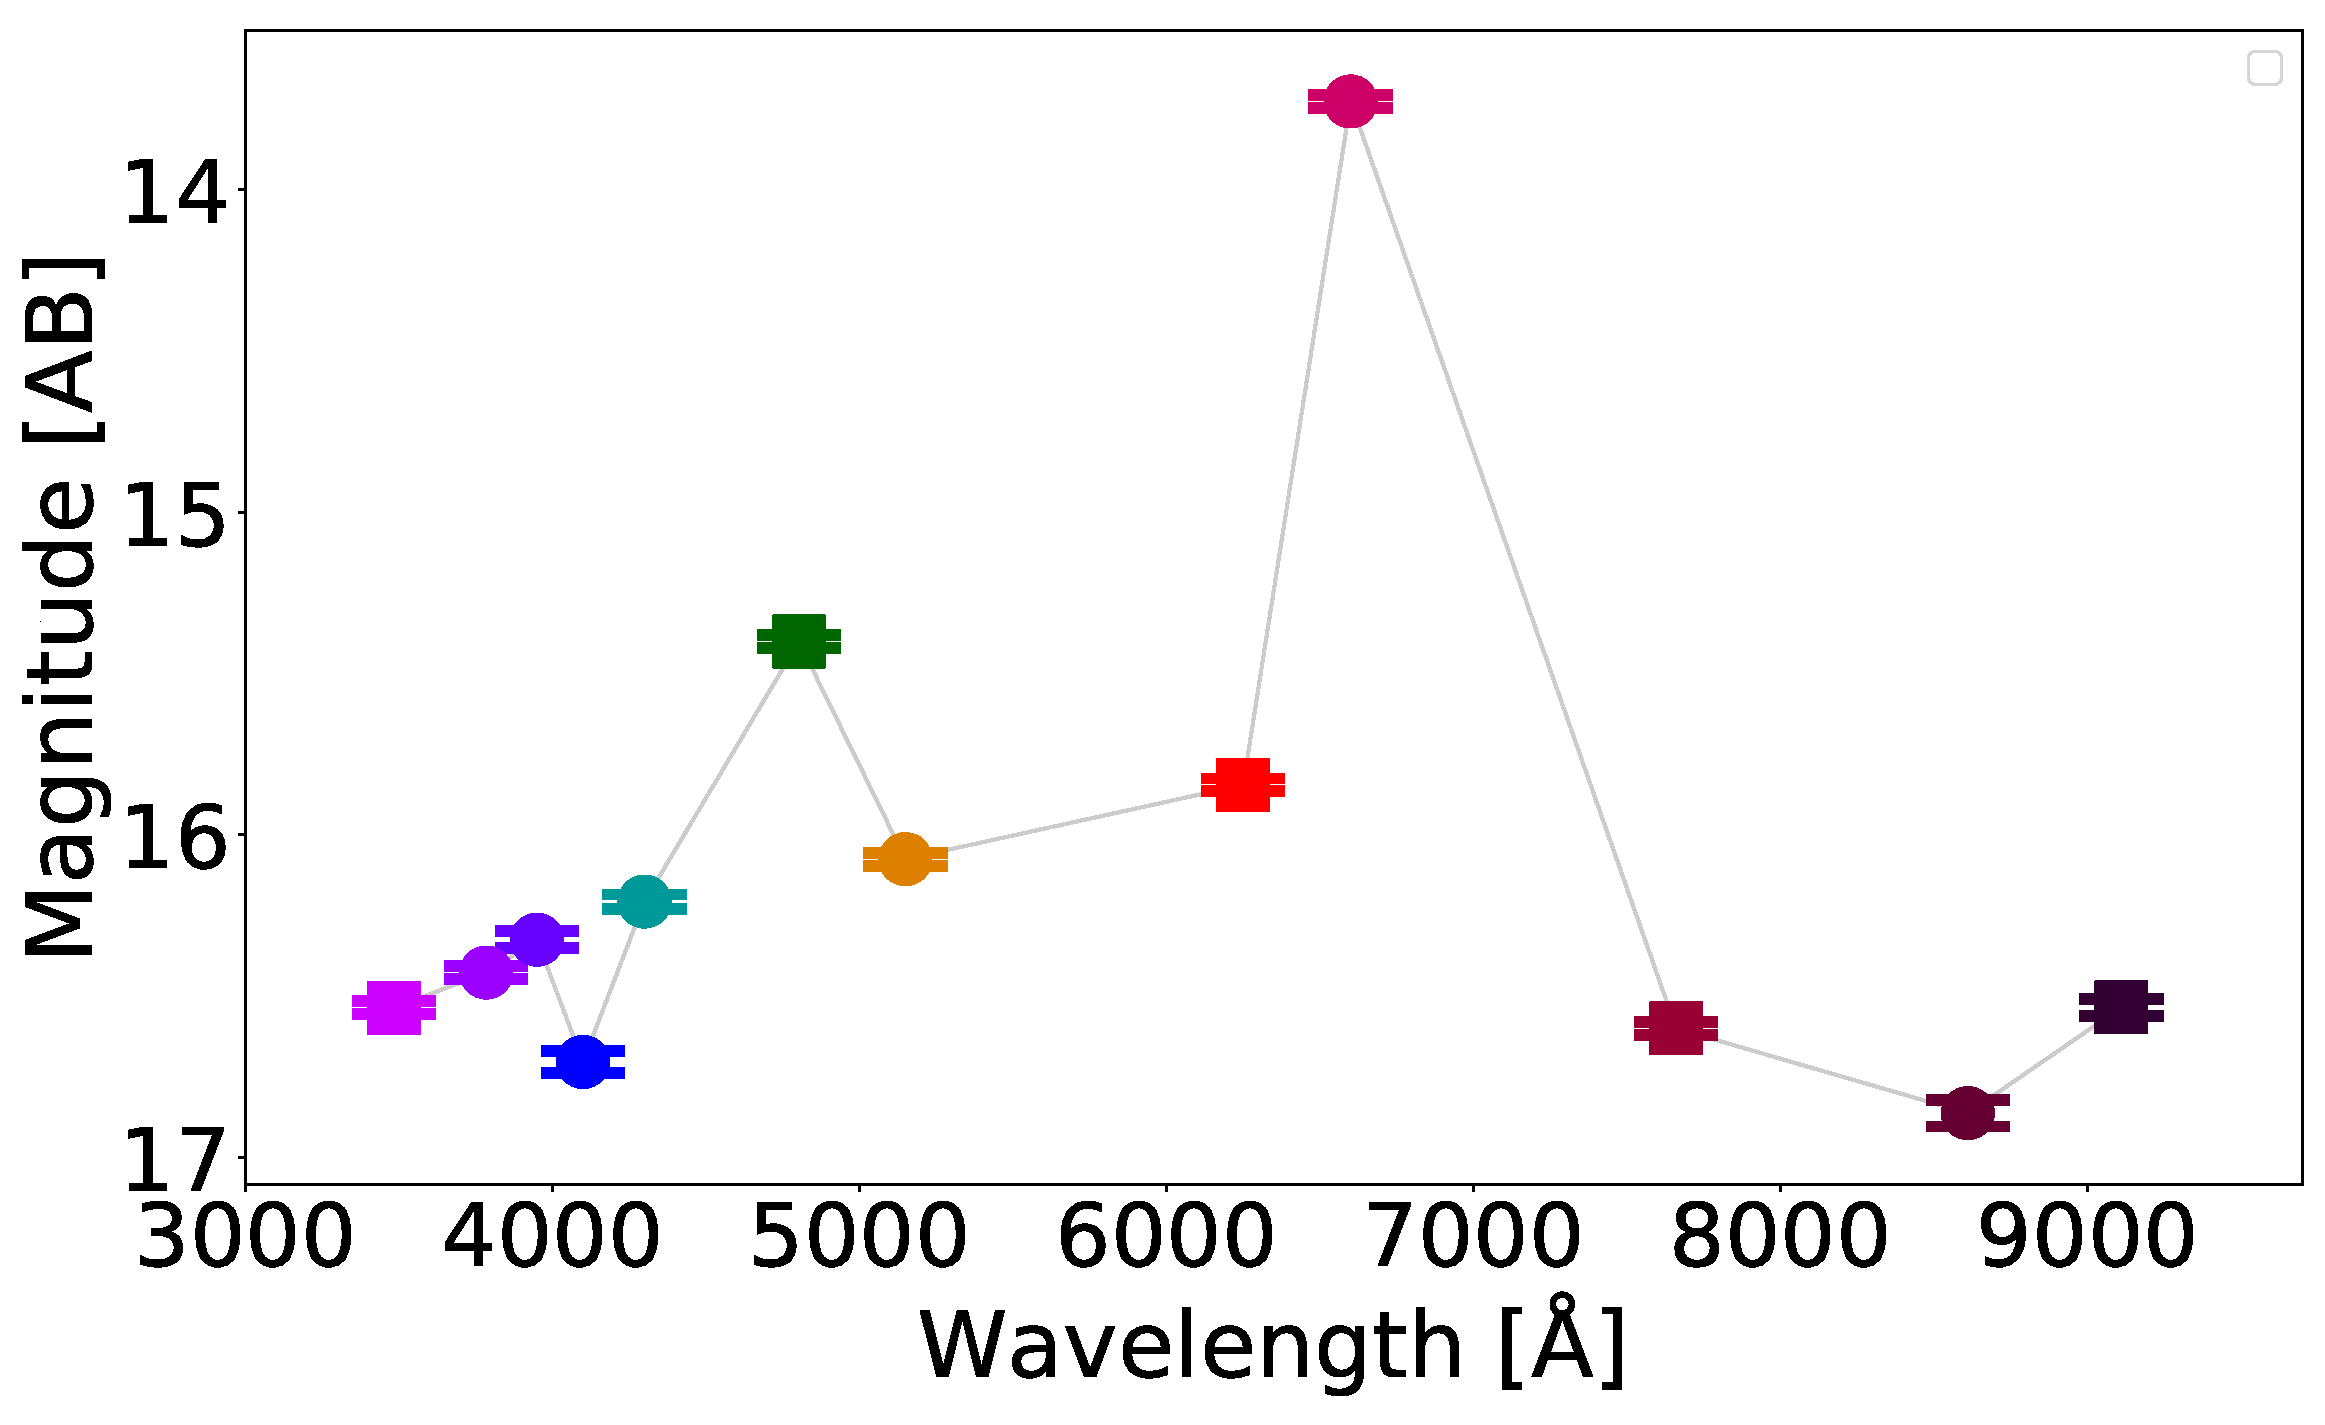
\includegraphics[width=0.3\linewidth, clip]{photopectrum_splus_MC0115-043944_auto.pdf} & 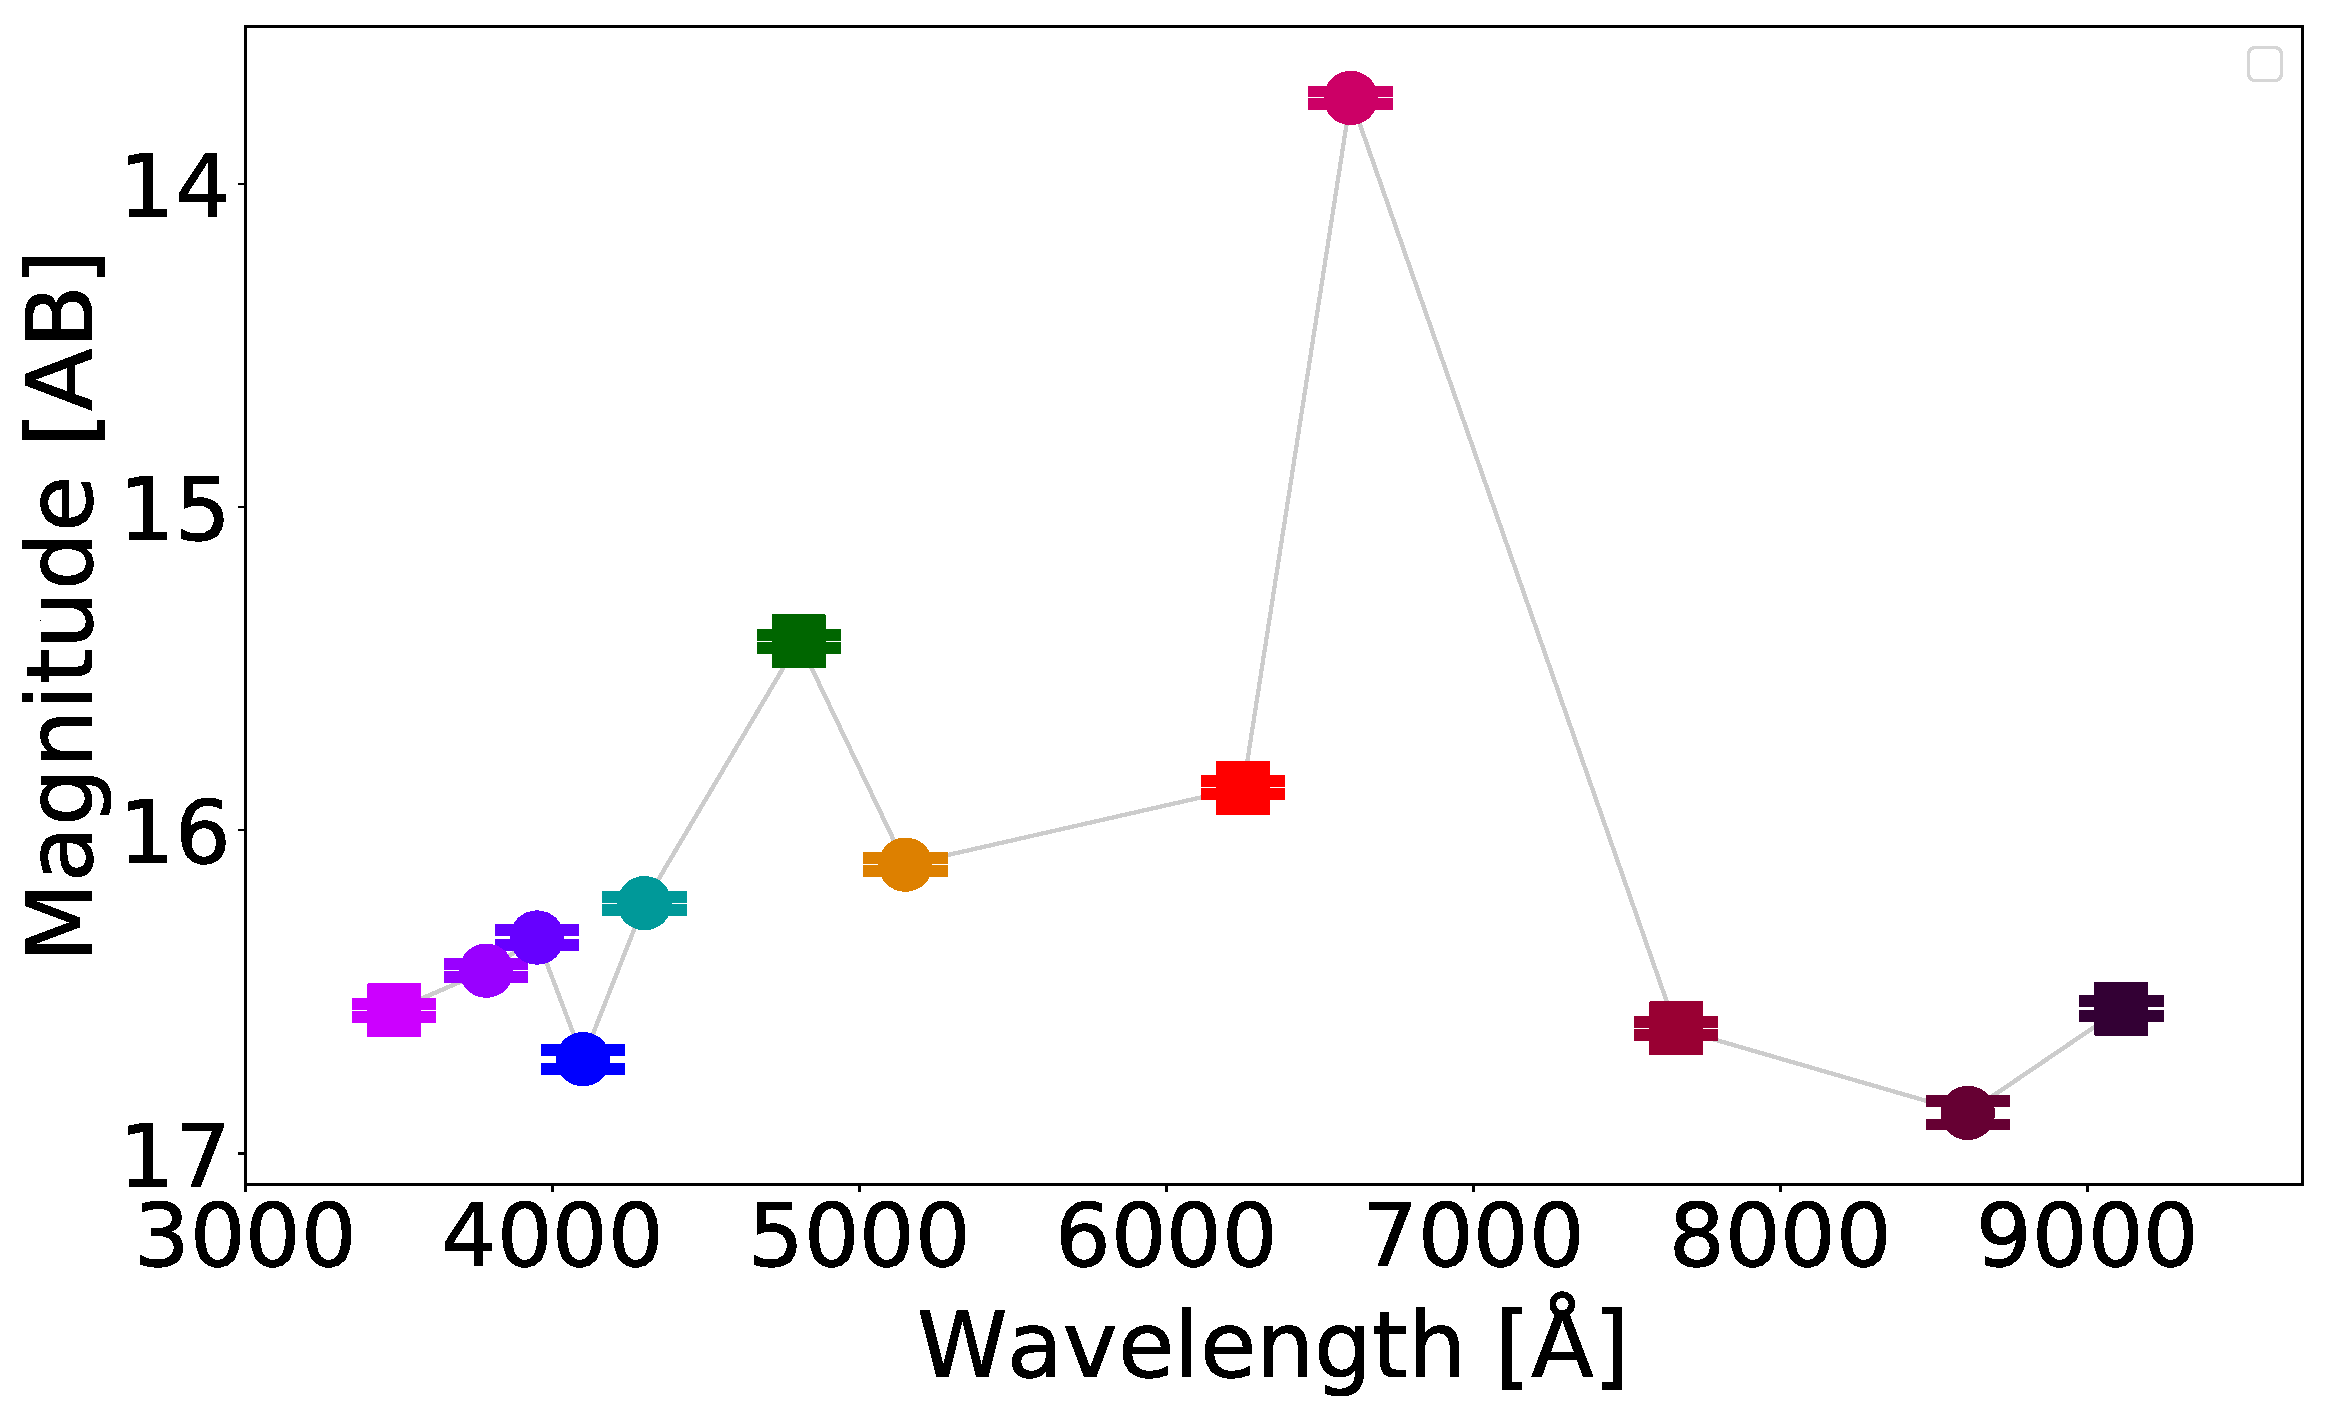
\includegraphics[width=0.3\linewidth, clip]{photopectrum_splus_MC0115-043944_petro.pdf} \\
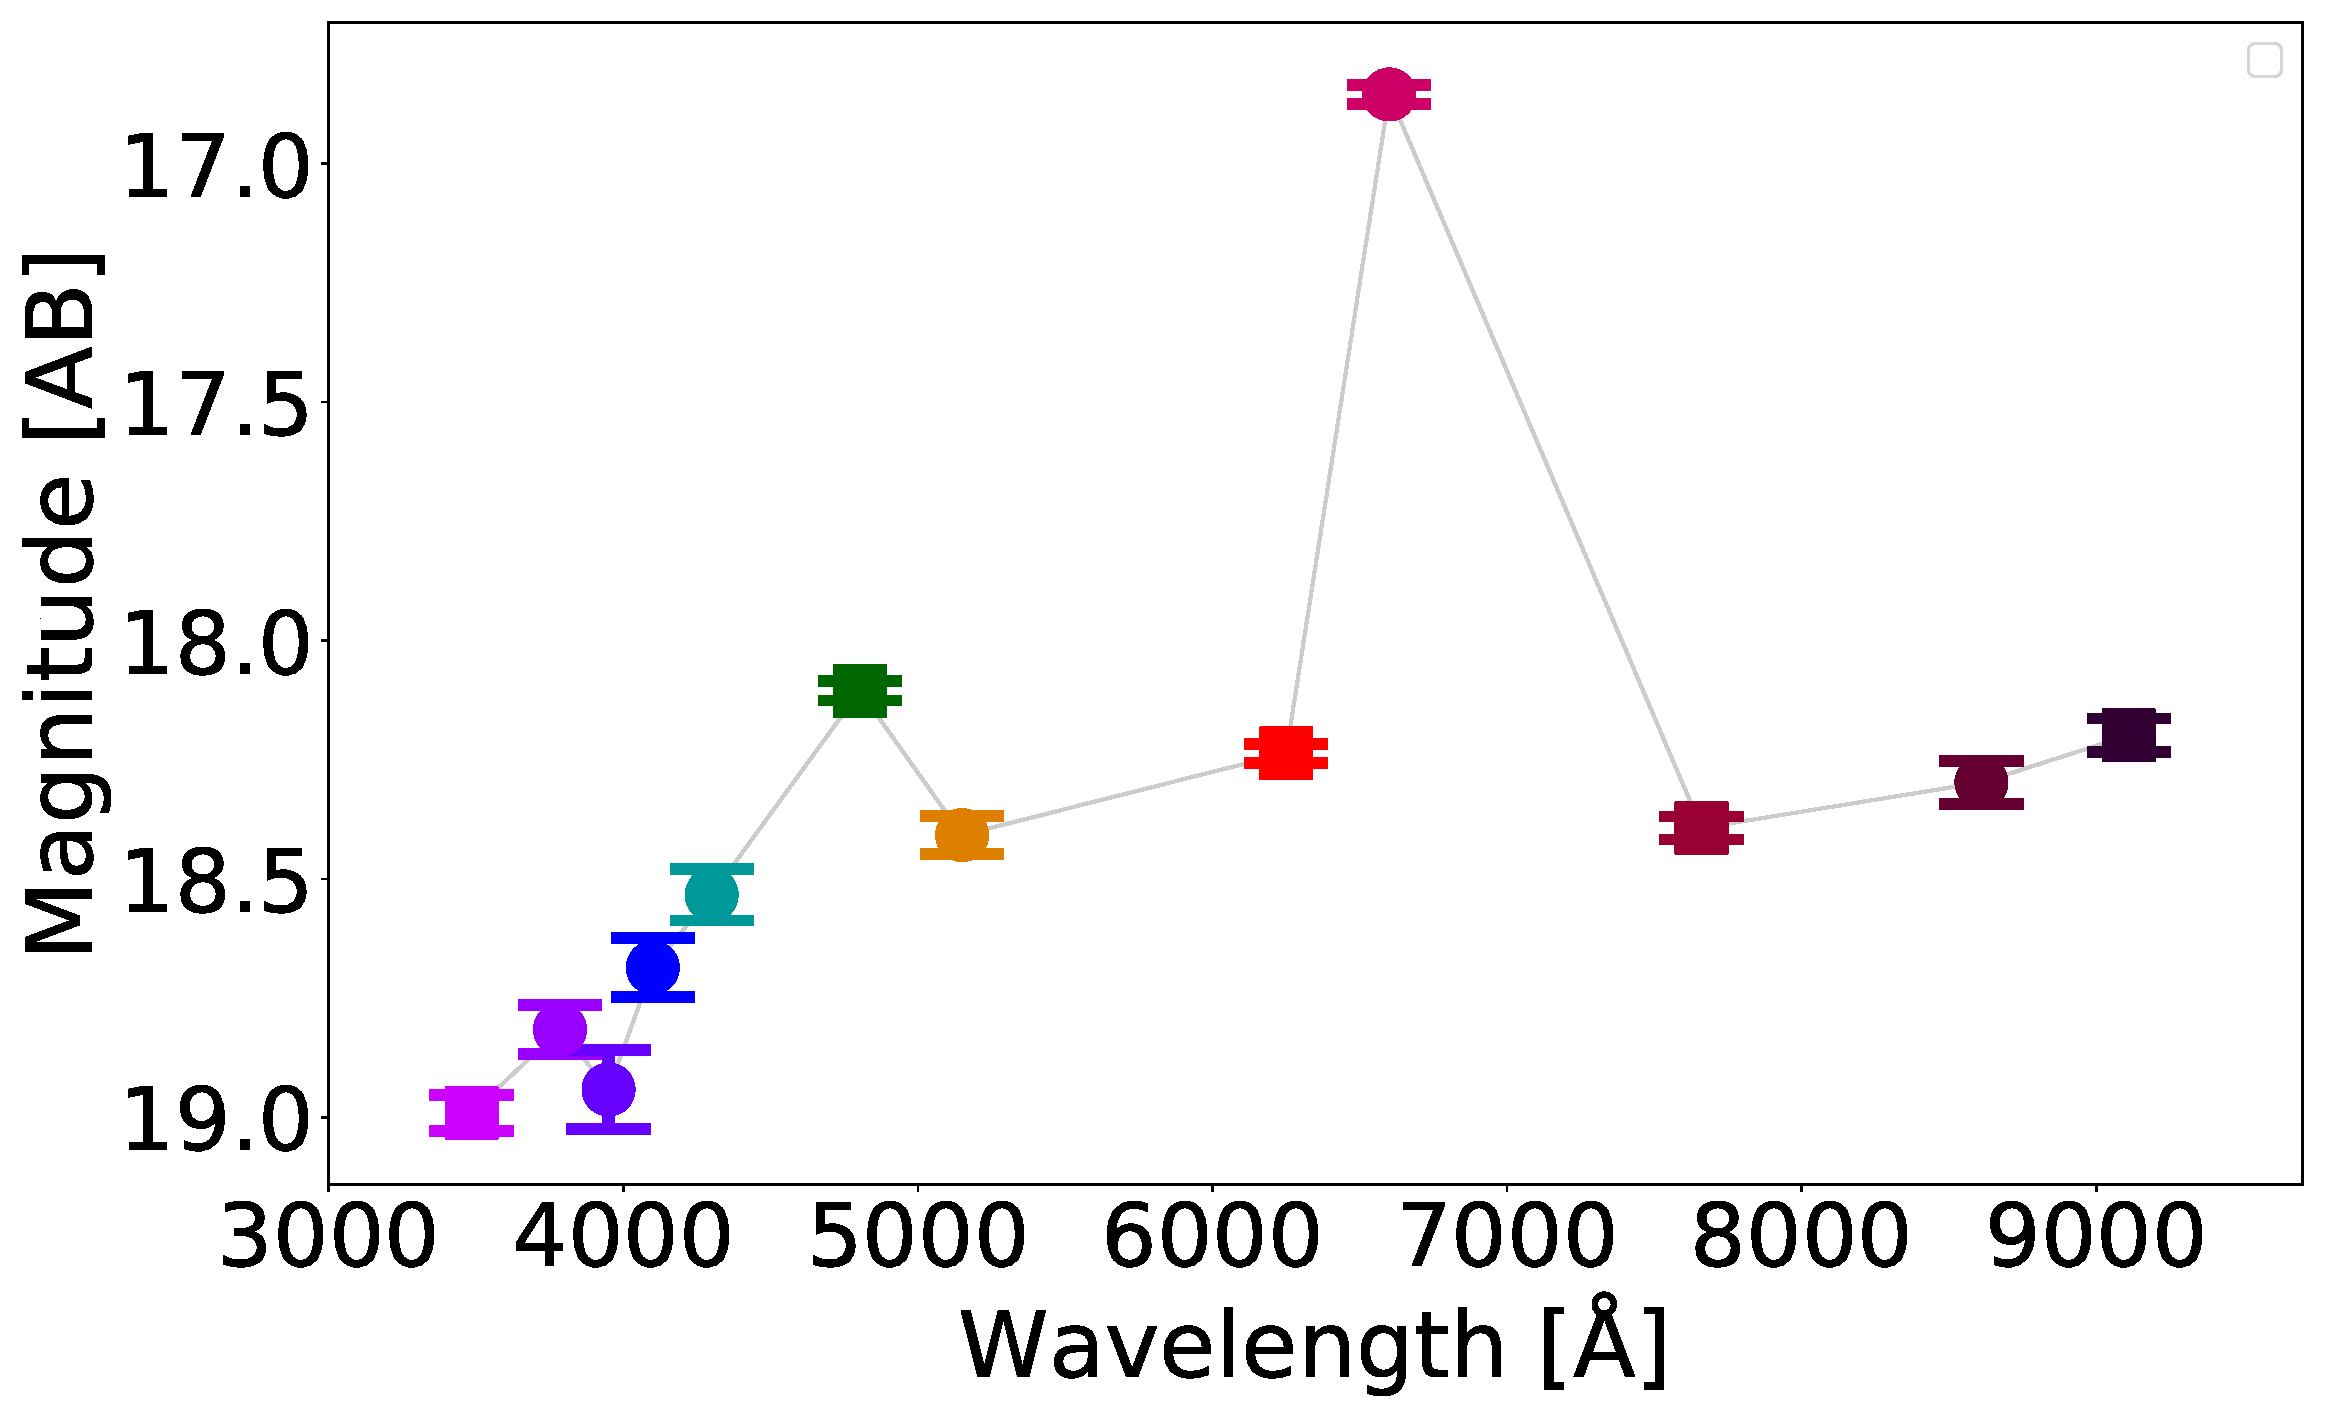
\includegraphics[width=0.3\linewidth, clip]{photopectrum_splus_MC0115-063029_aper.pdf} & 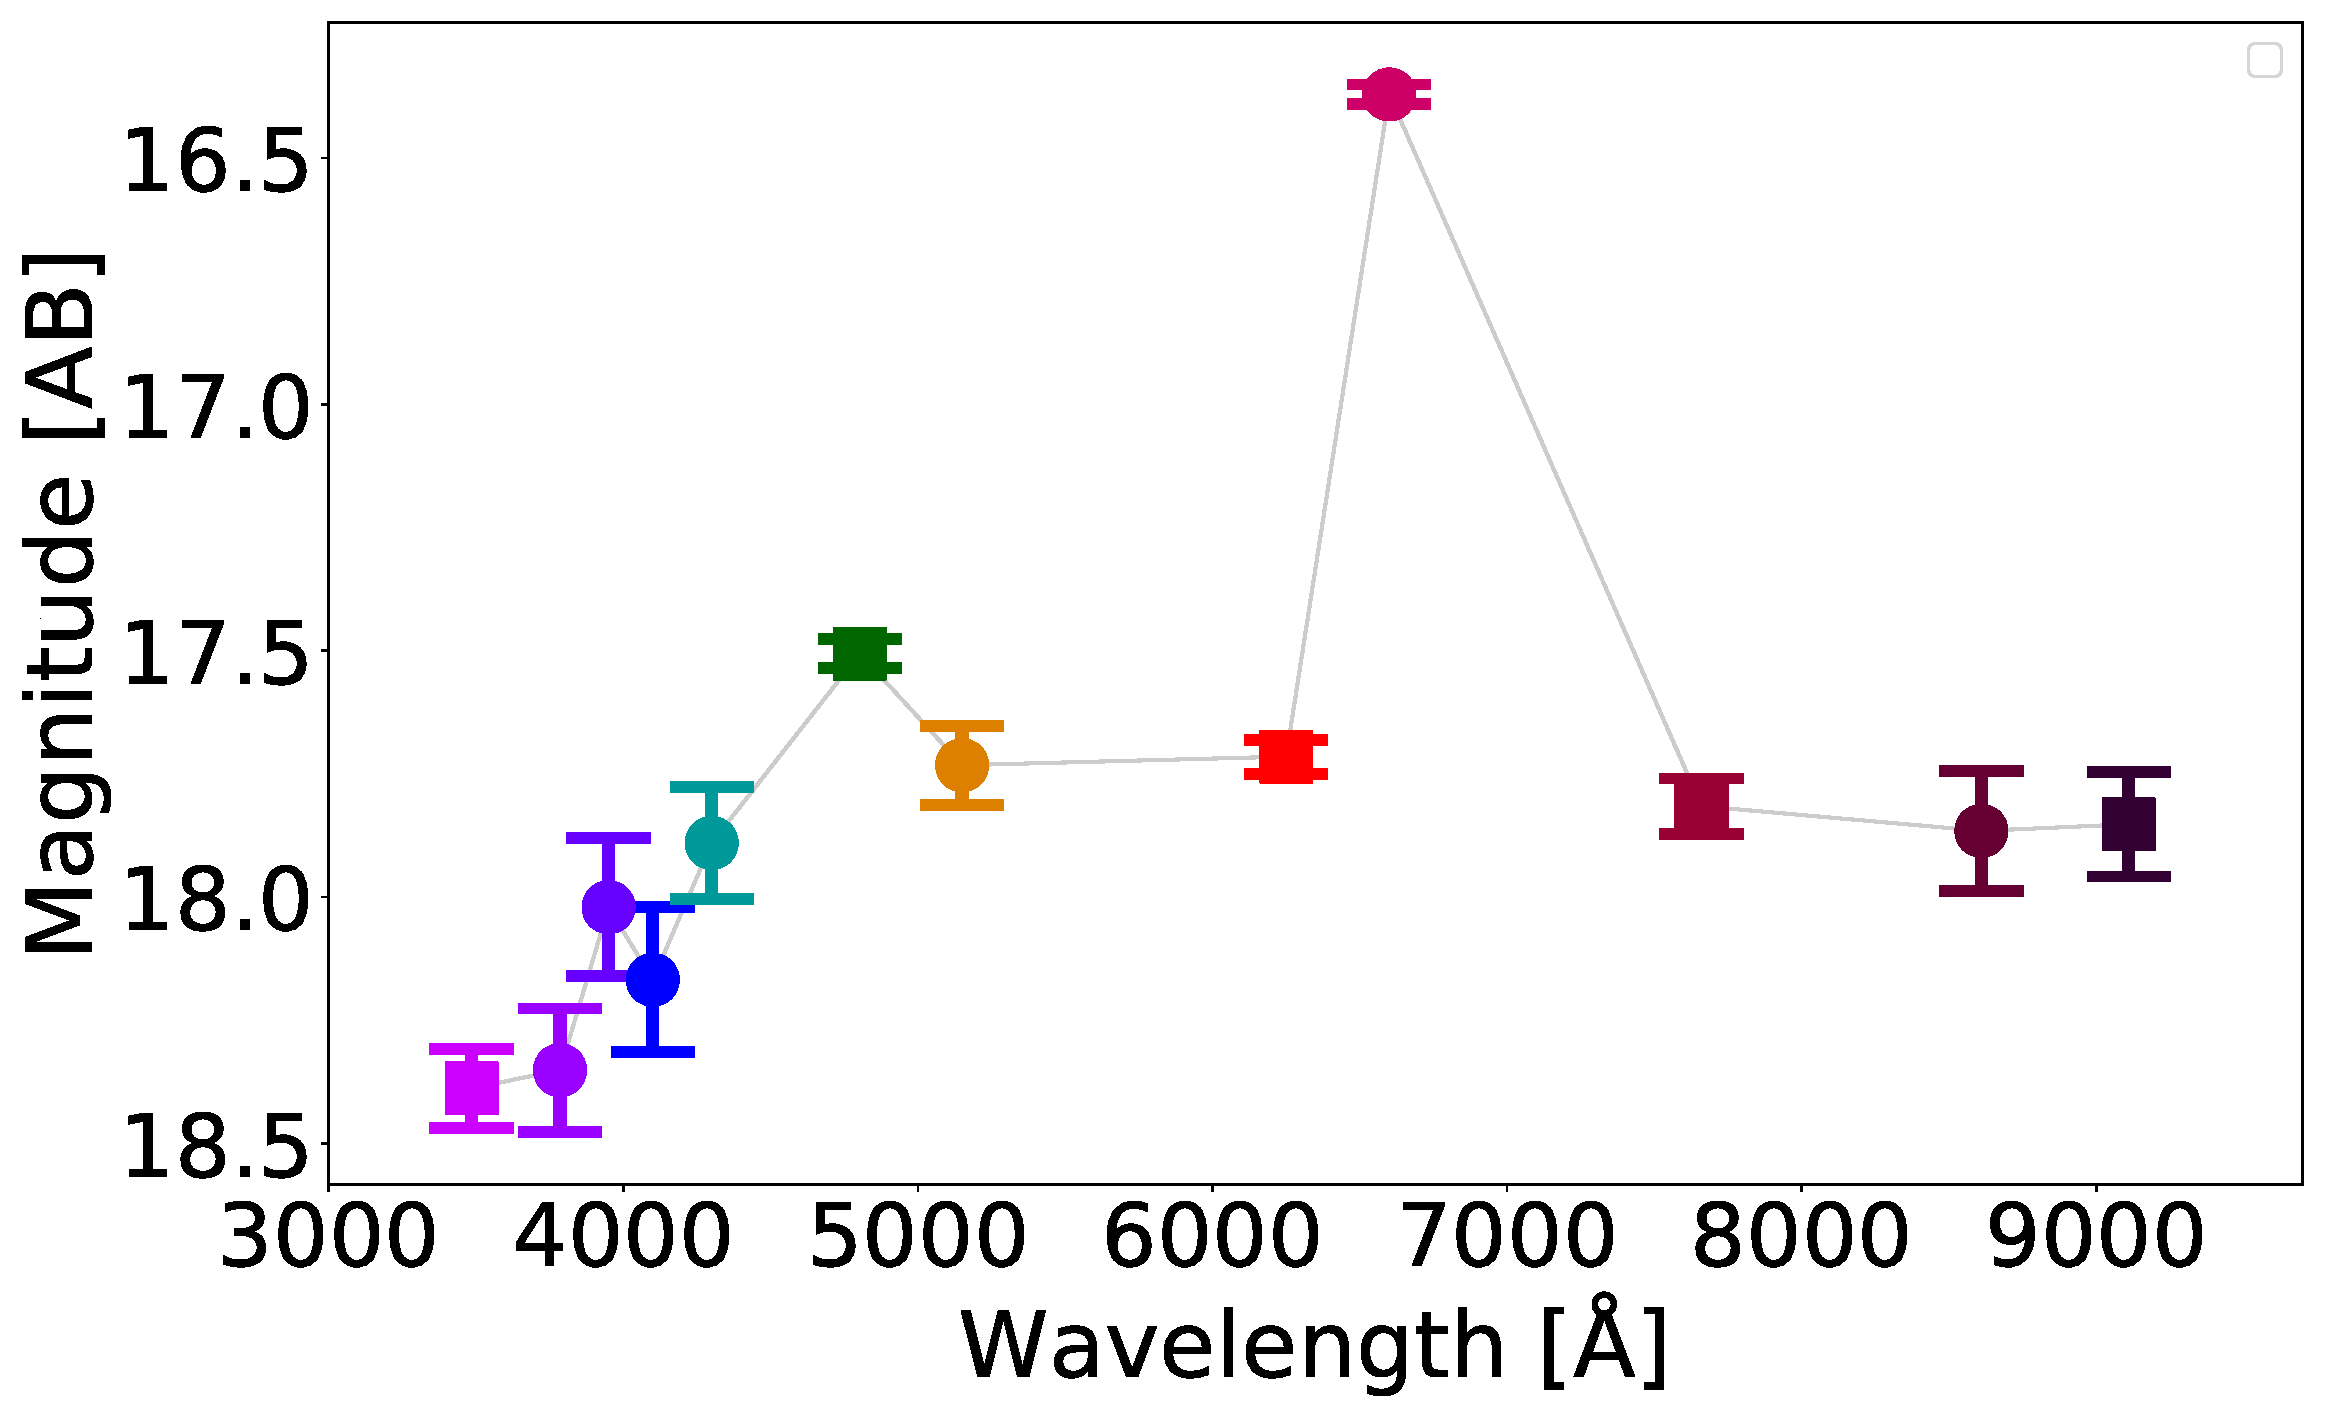
\includegraphics[width=0.3\linewidth, clip]{photopectrum_splus_MC0115-063029_auto.pdf} & 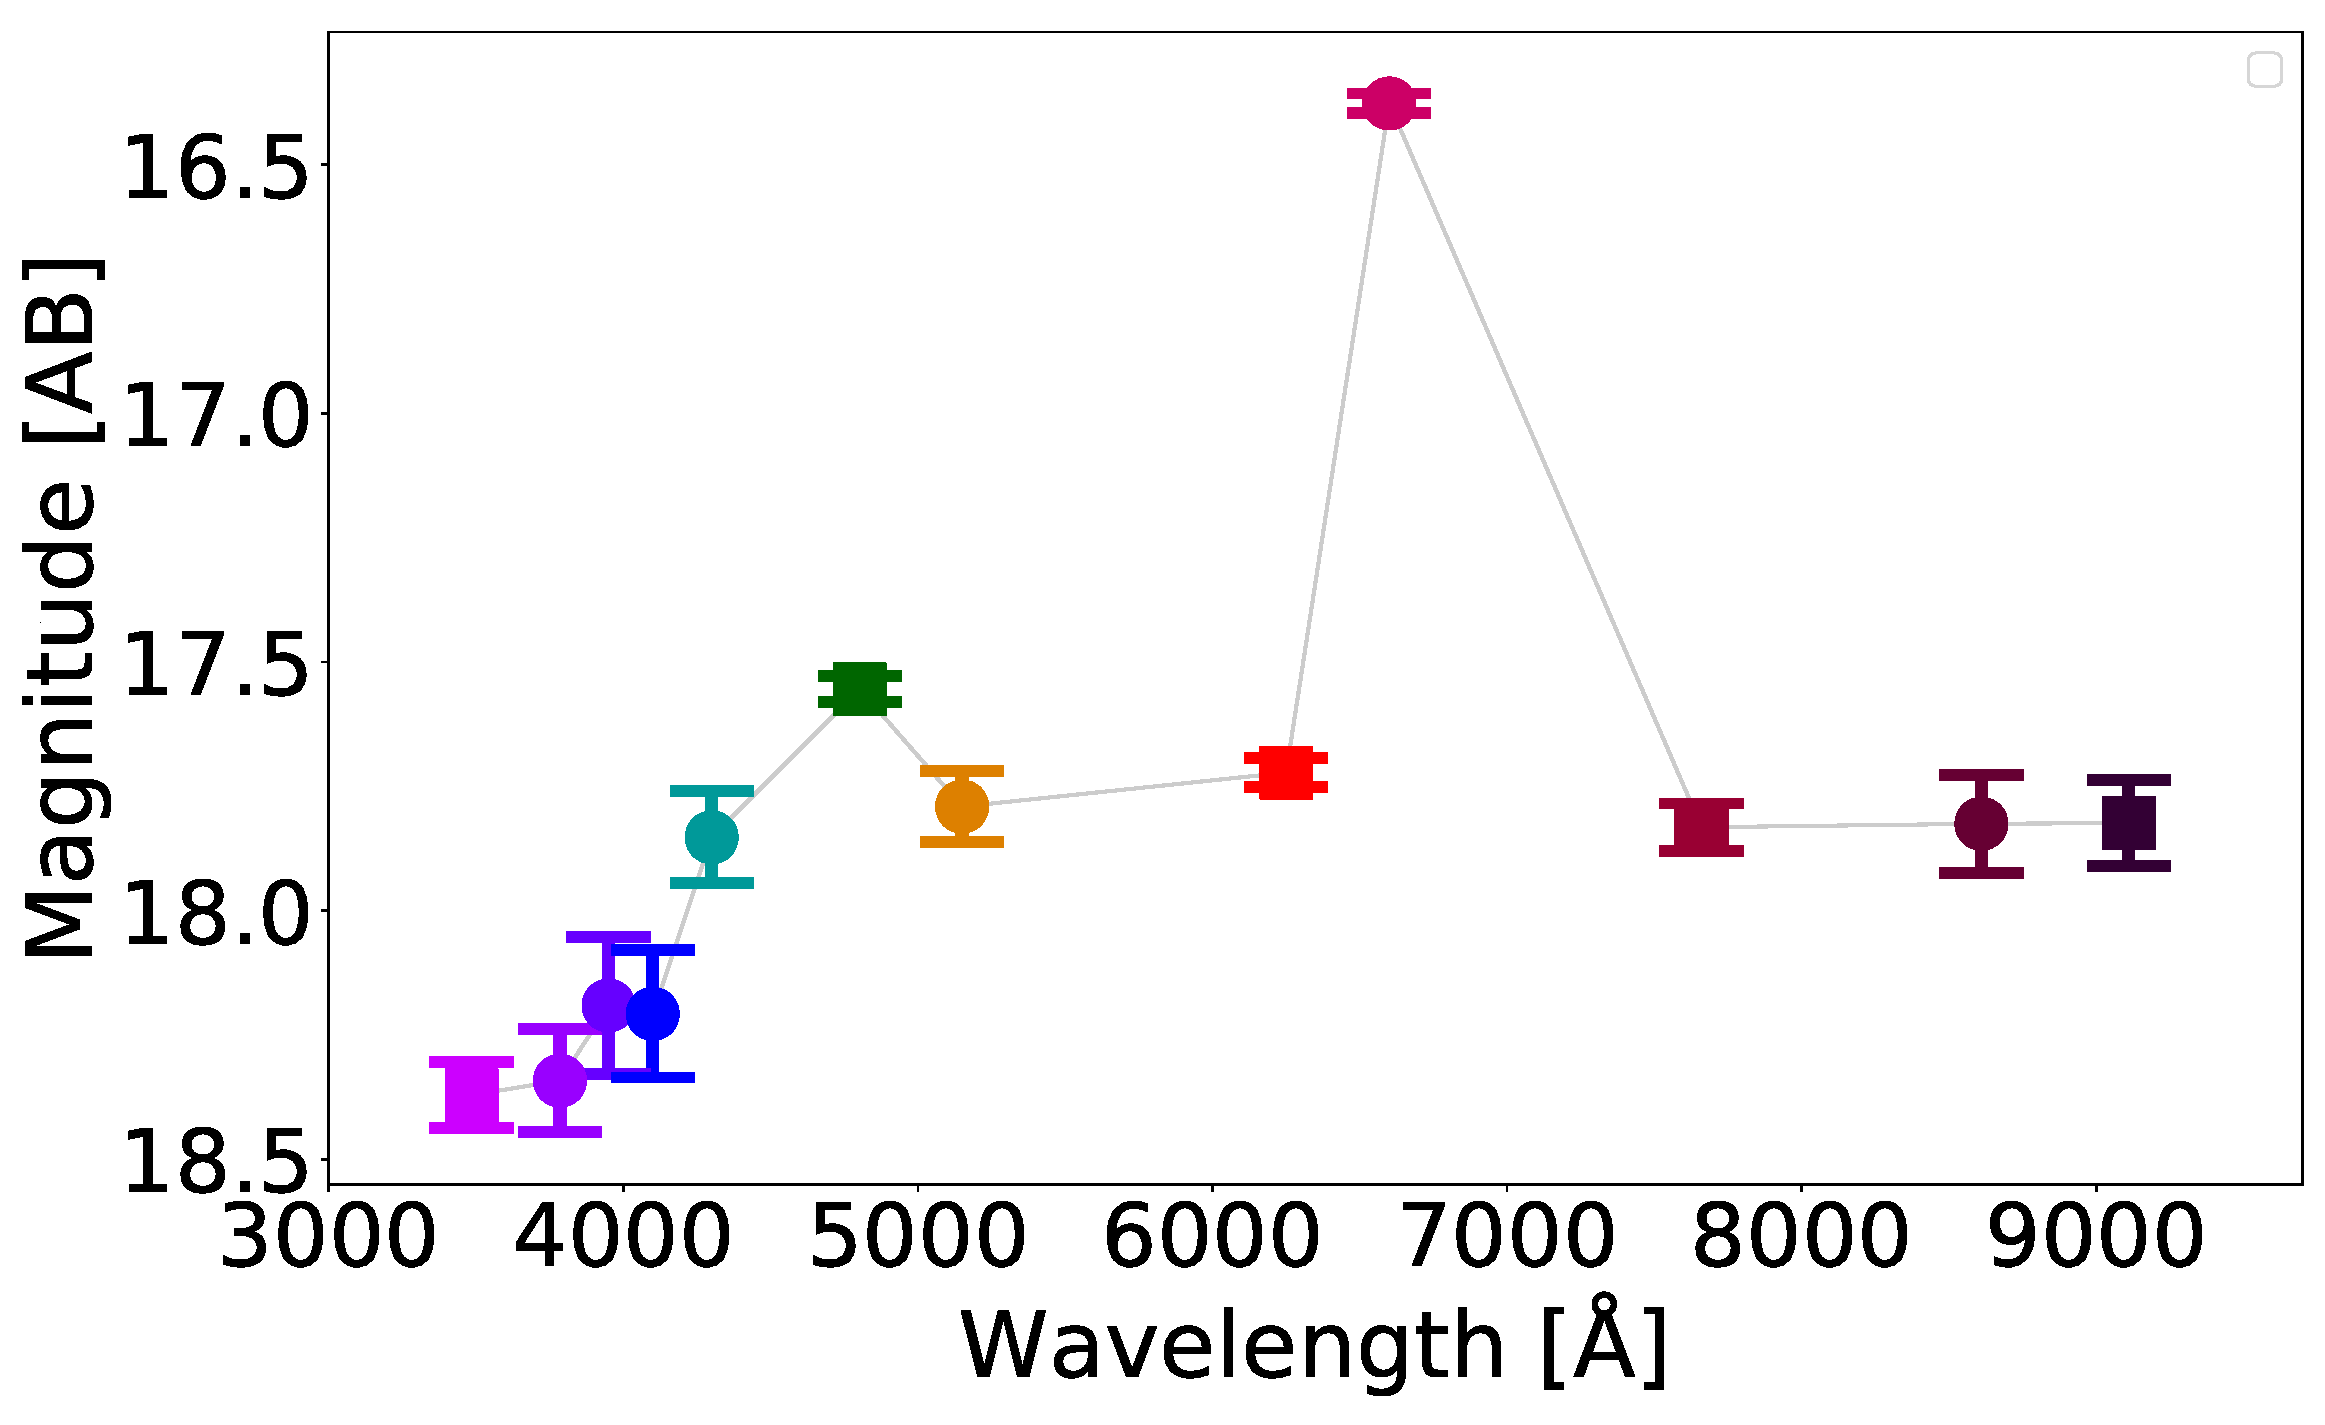
\includegraphics[width=0.3\linewidth, clip]{photopectrum_splus_MC0115-063029_petro.pdf} \\
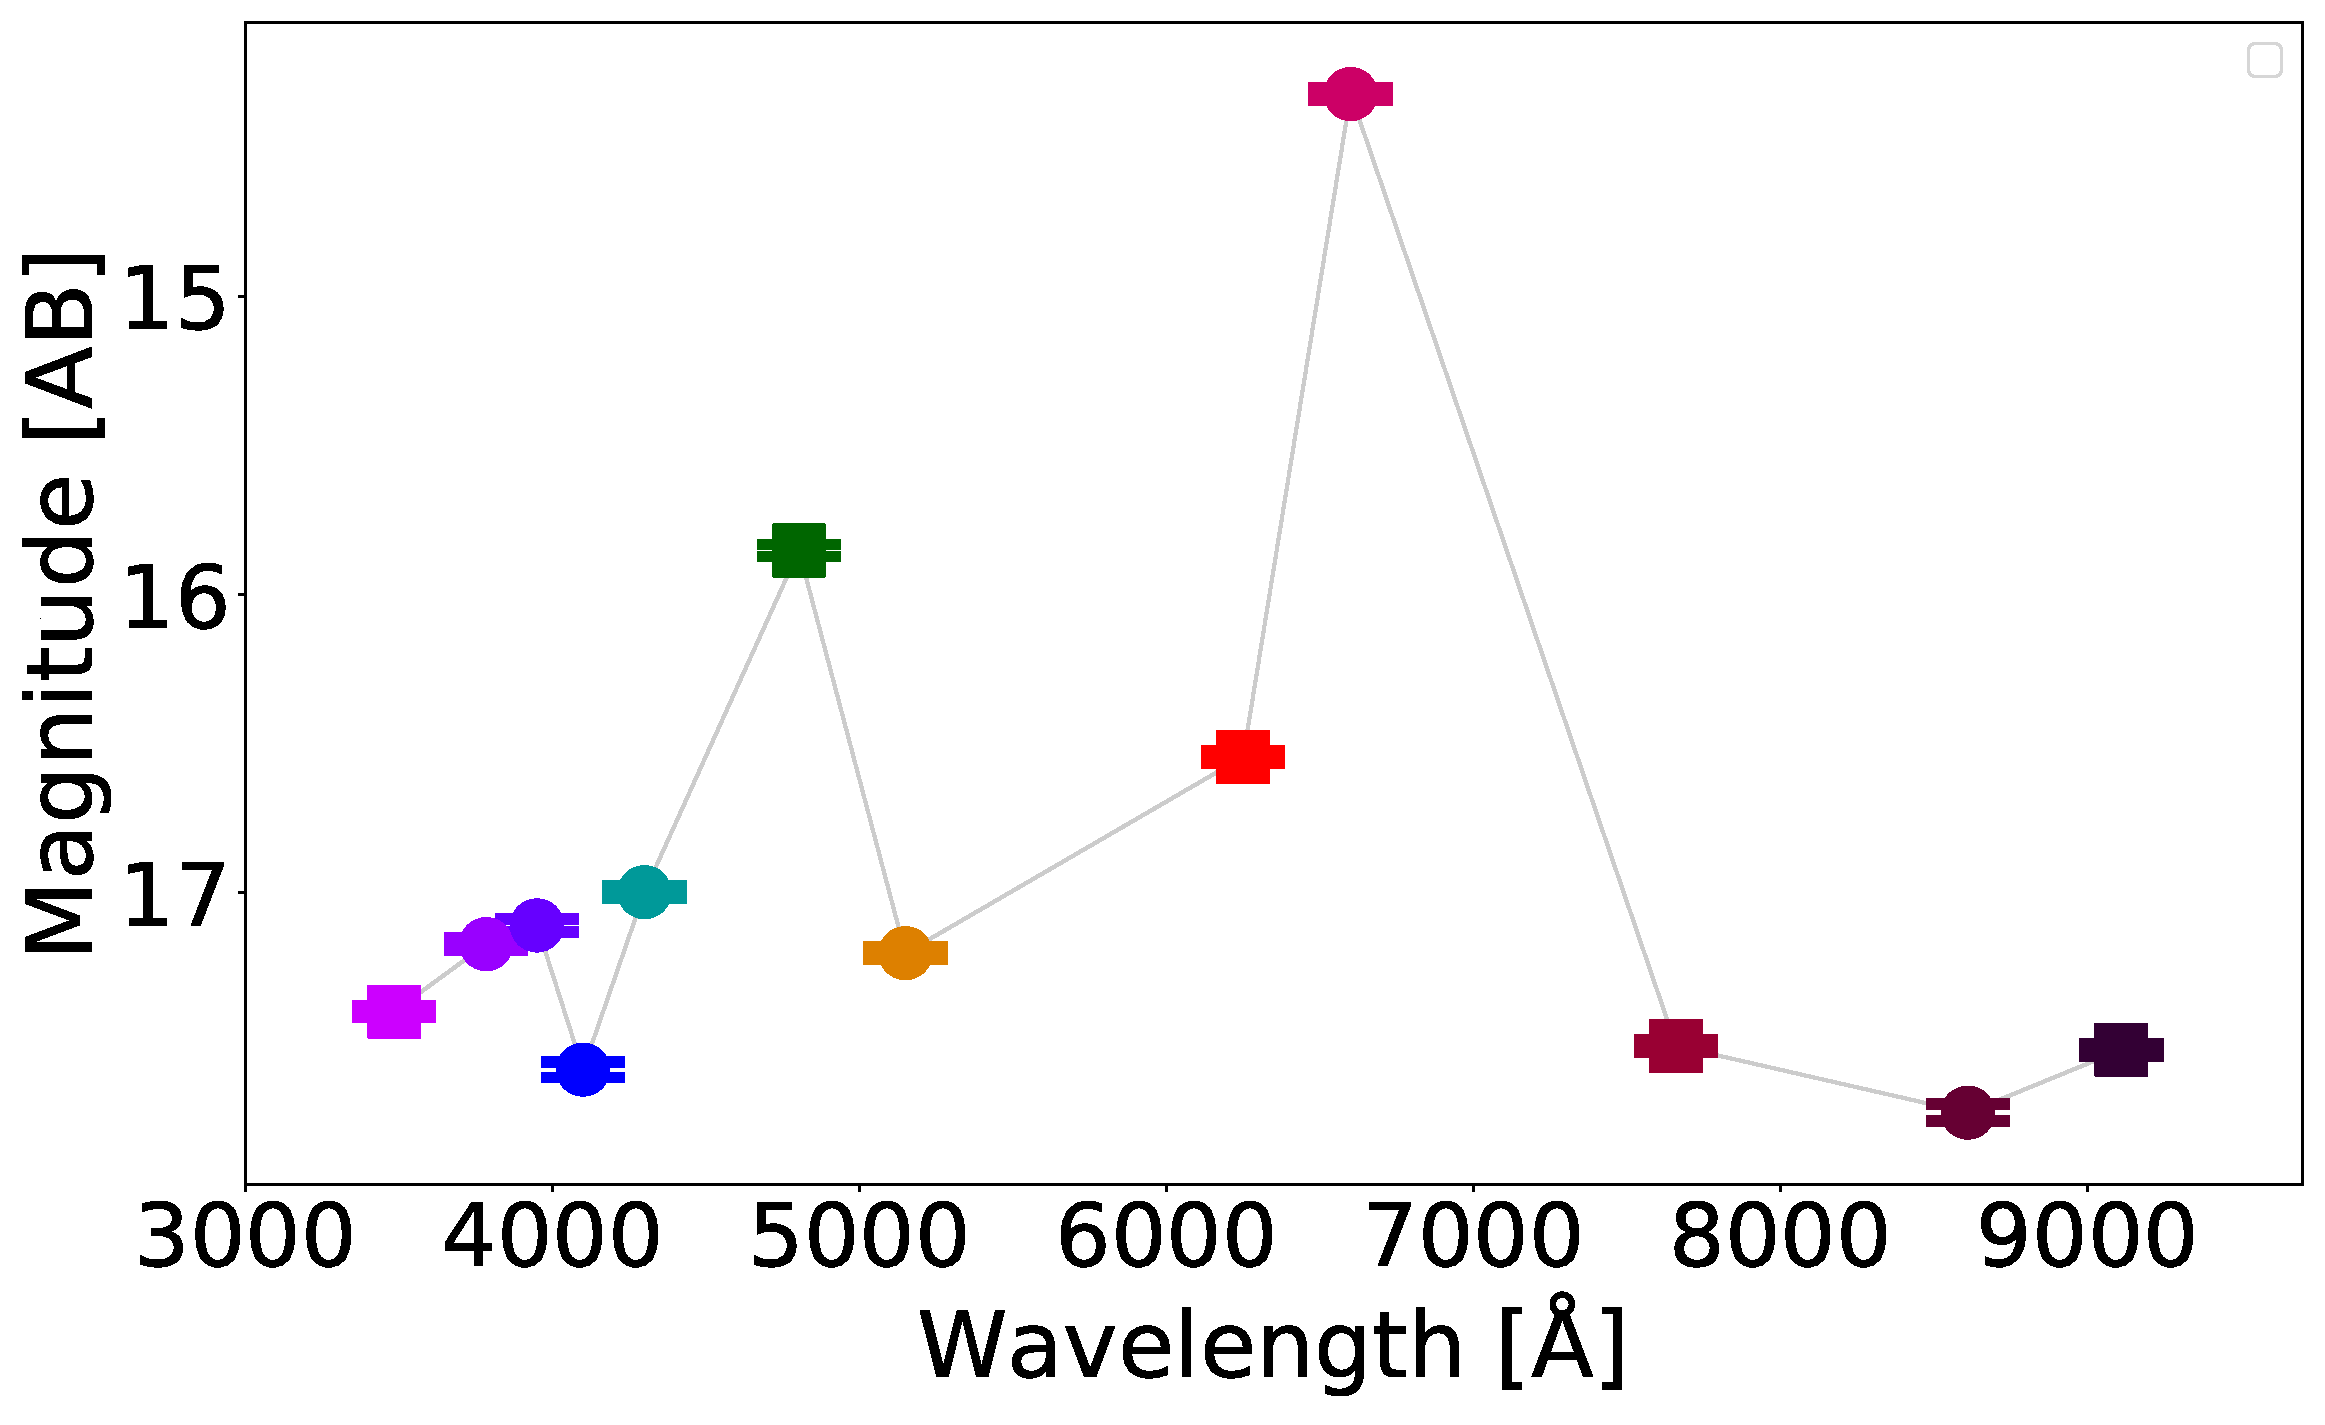
\includegraphics[width=0.3\linewidth, clip]{photopectrum_splus_MC0115-105523_aper.pdf} & 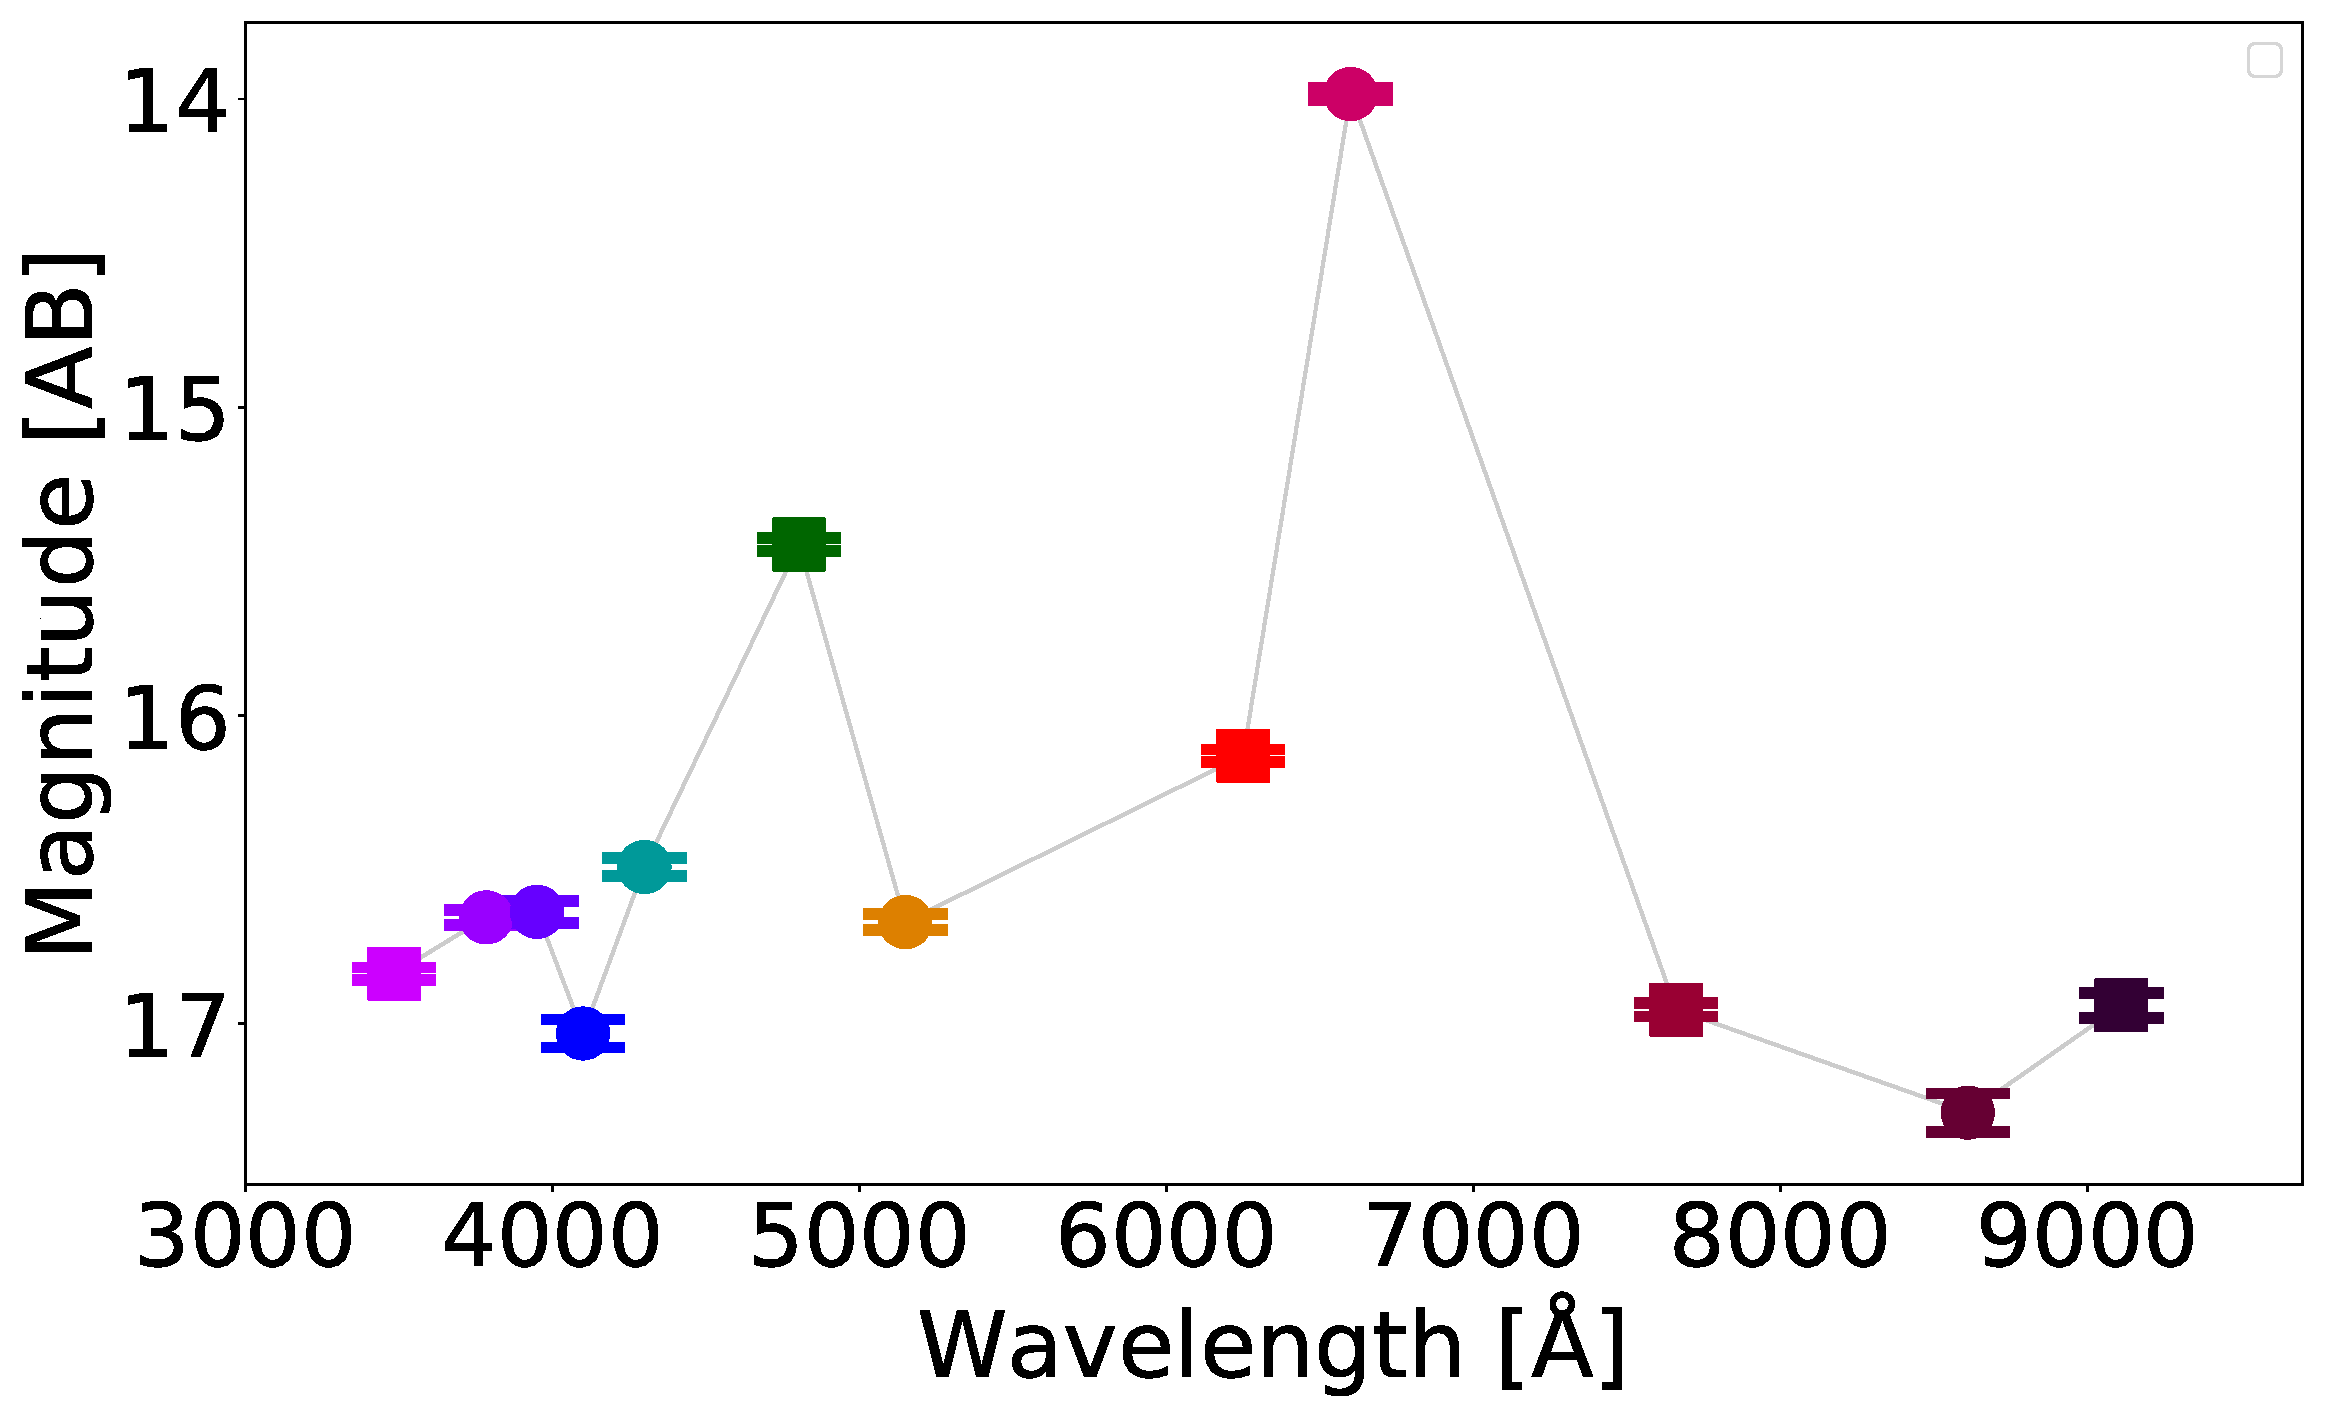
\includegraphics[width=0.3\linewidth, clip]{photopectrum_splus_MC0115-105523_auto.pdf} & 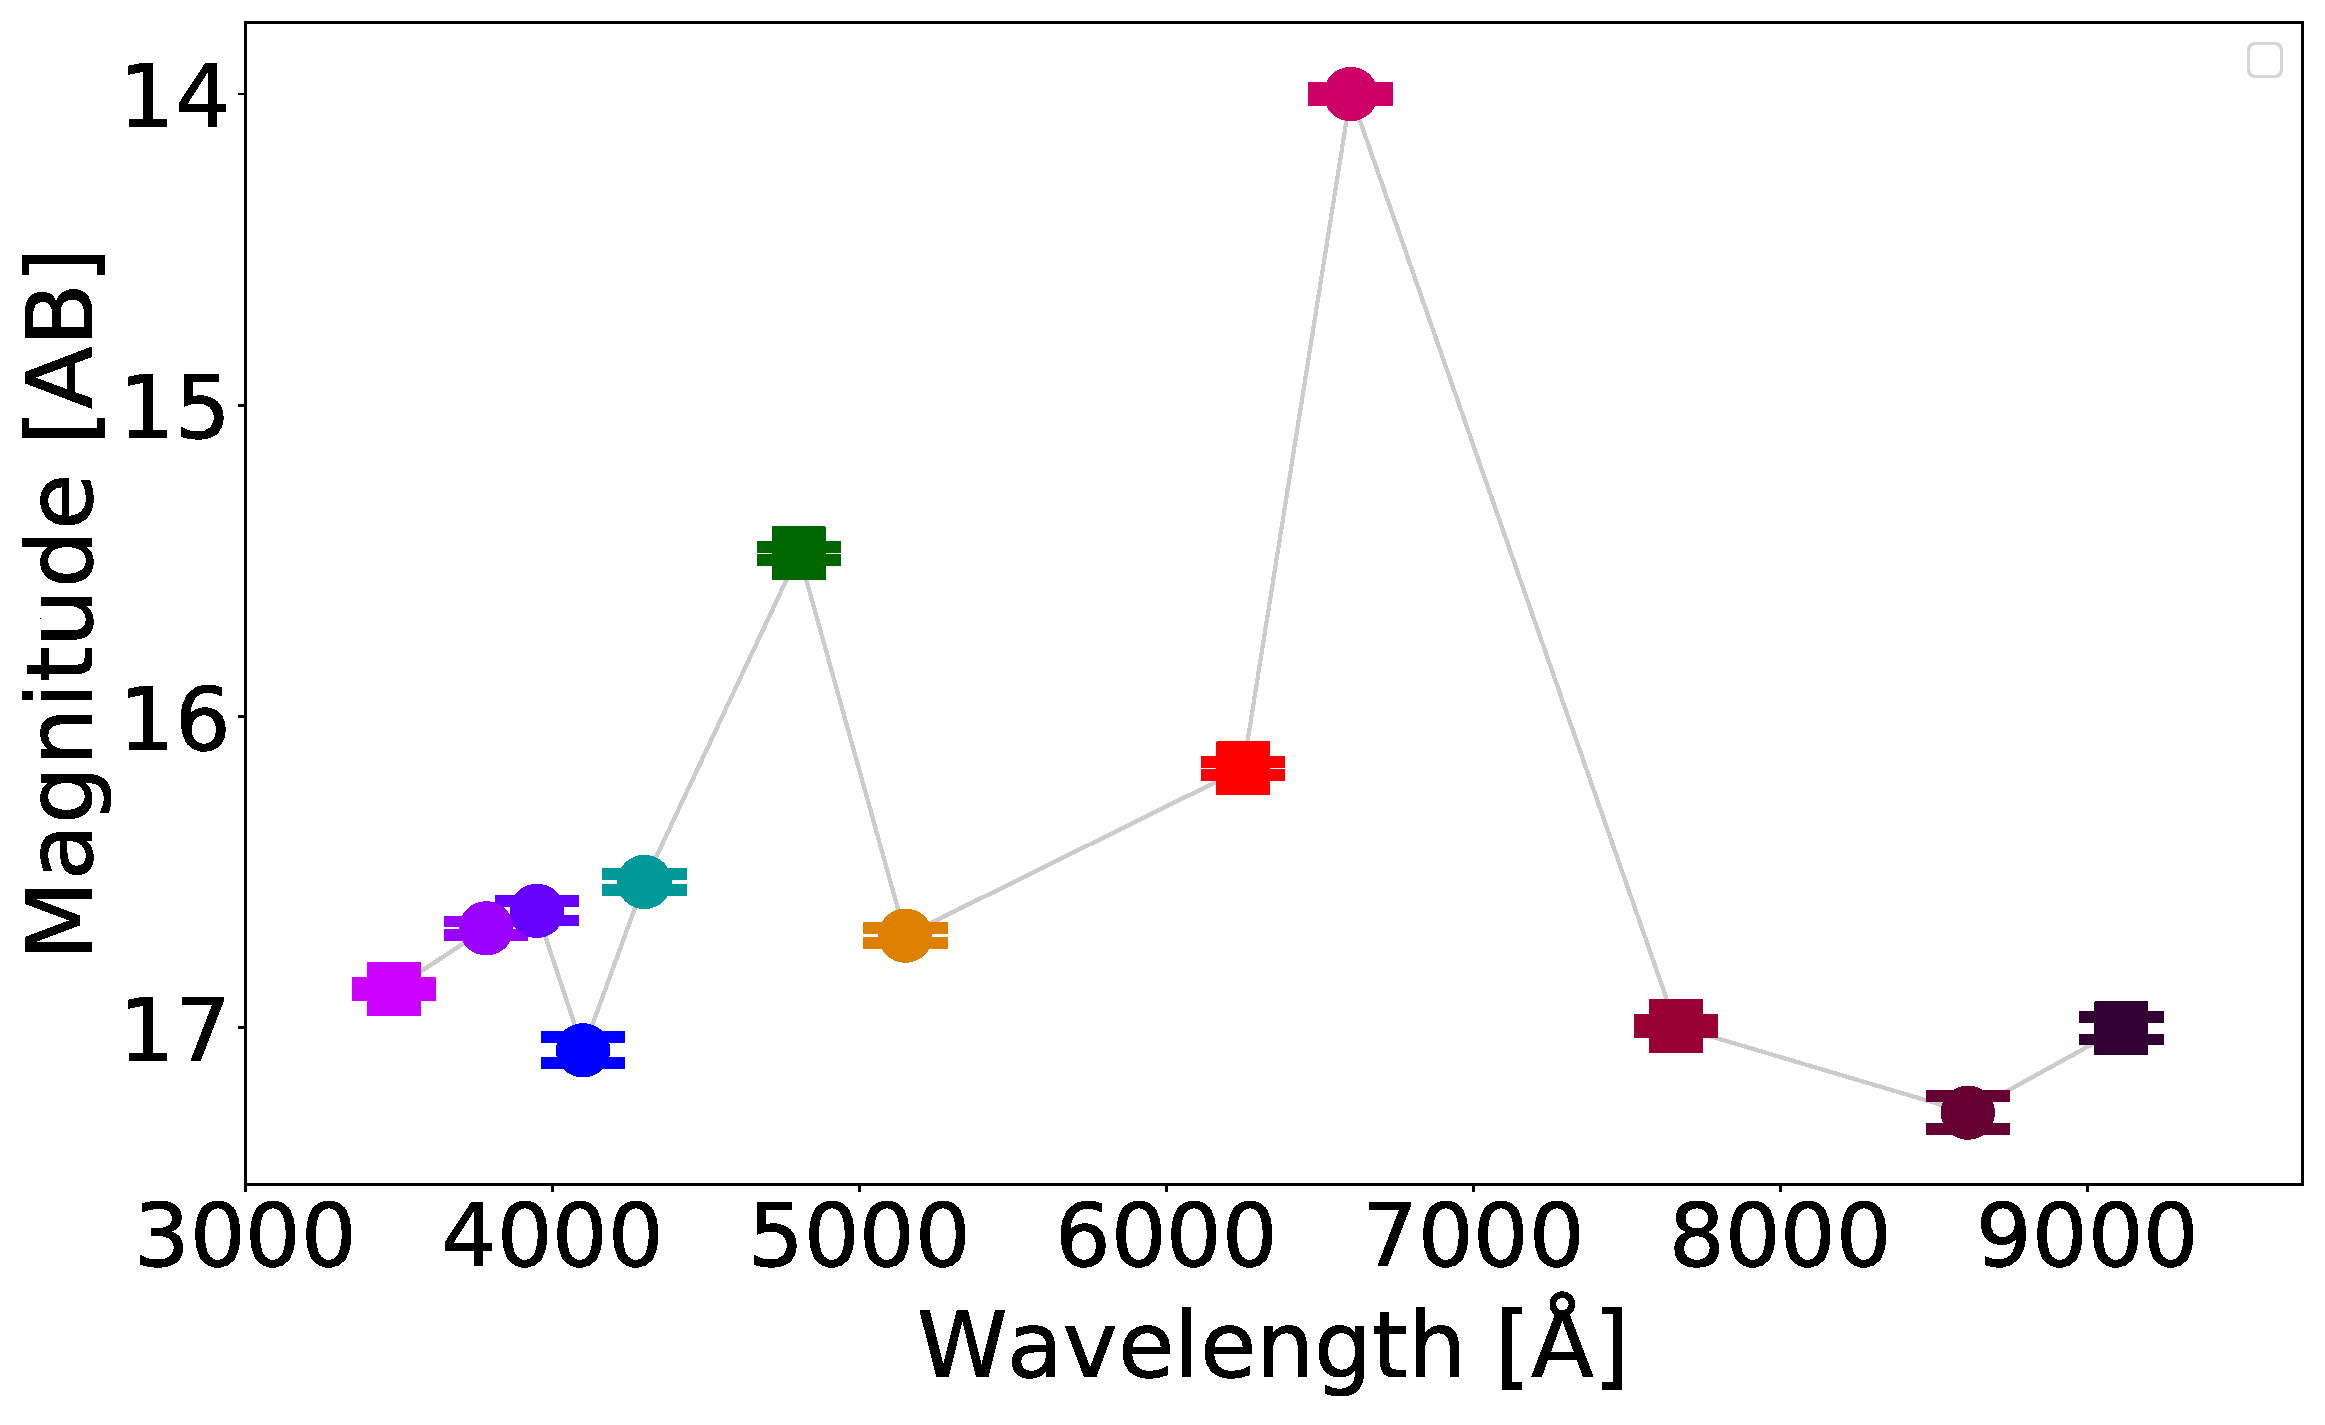
\includegraphics[width=0.3\linewidth, clip]{photopectrum_splus_MC0115-105523_petro.pdf} \\
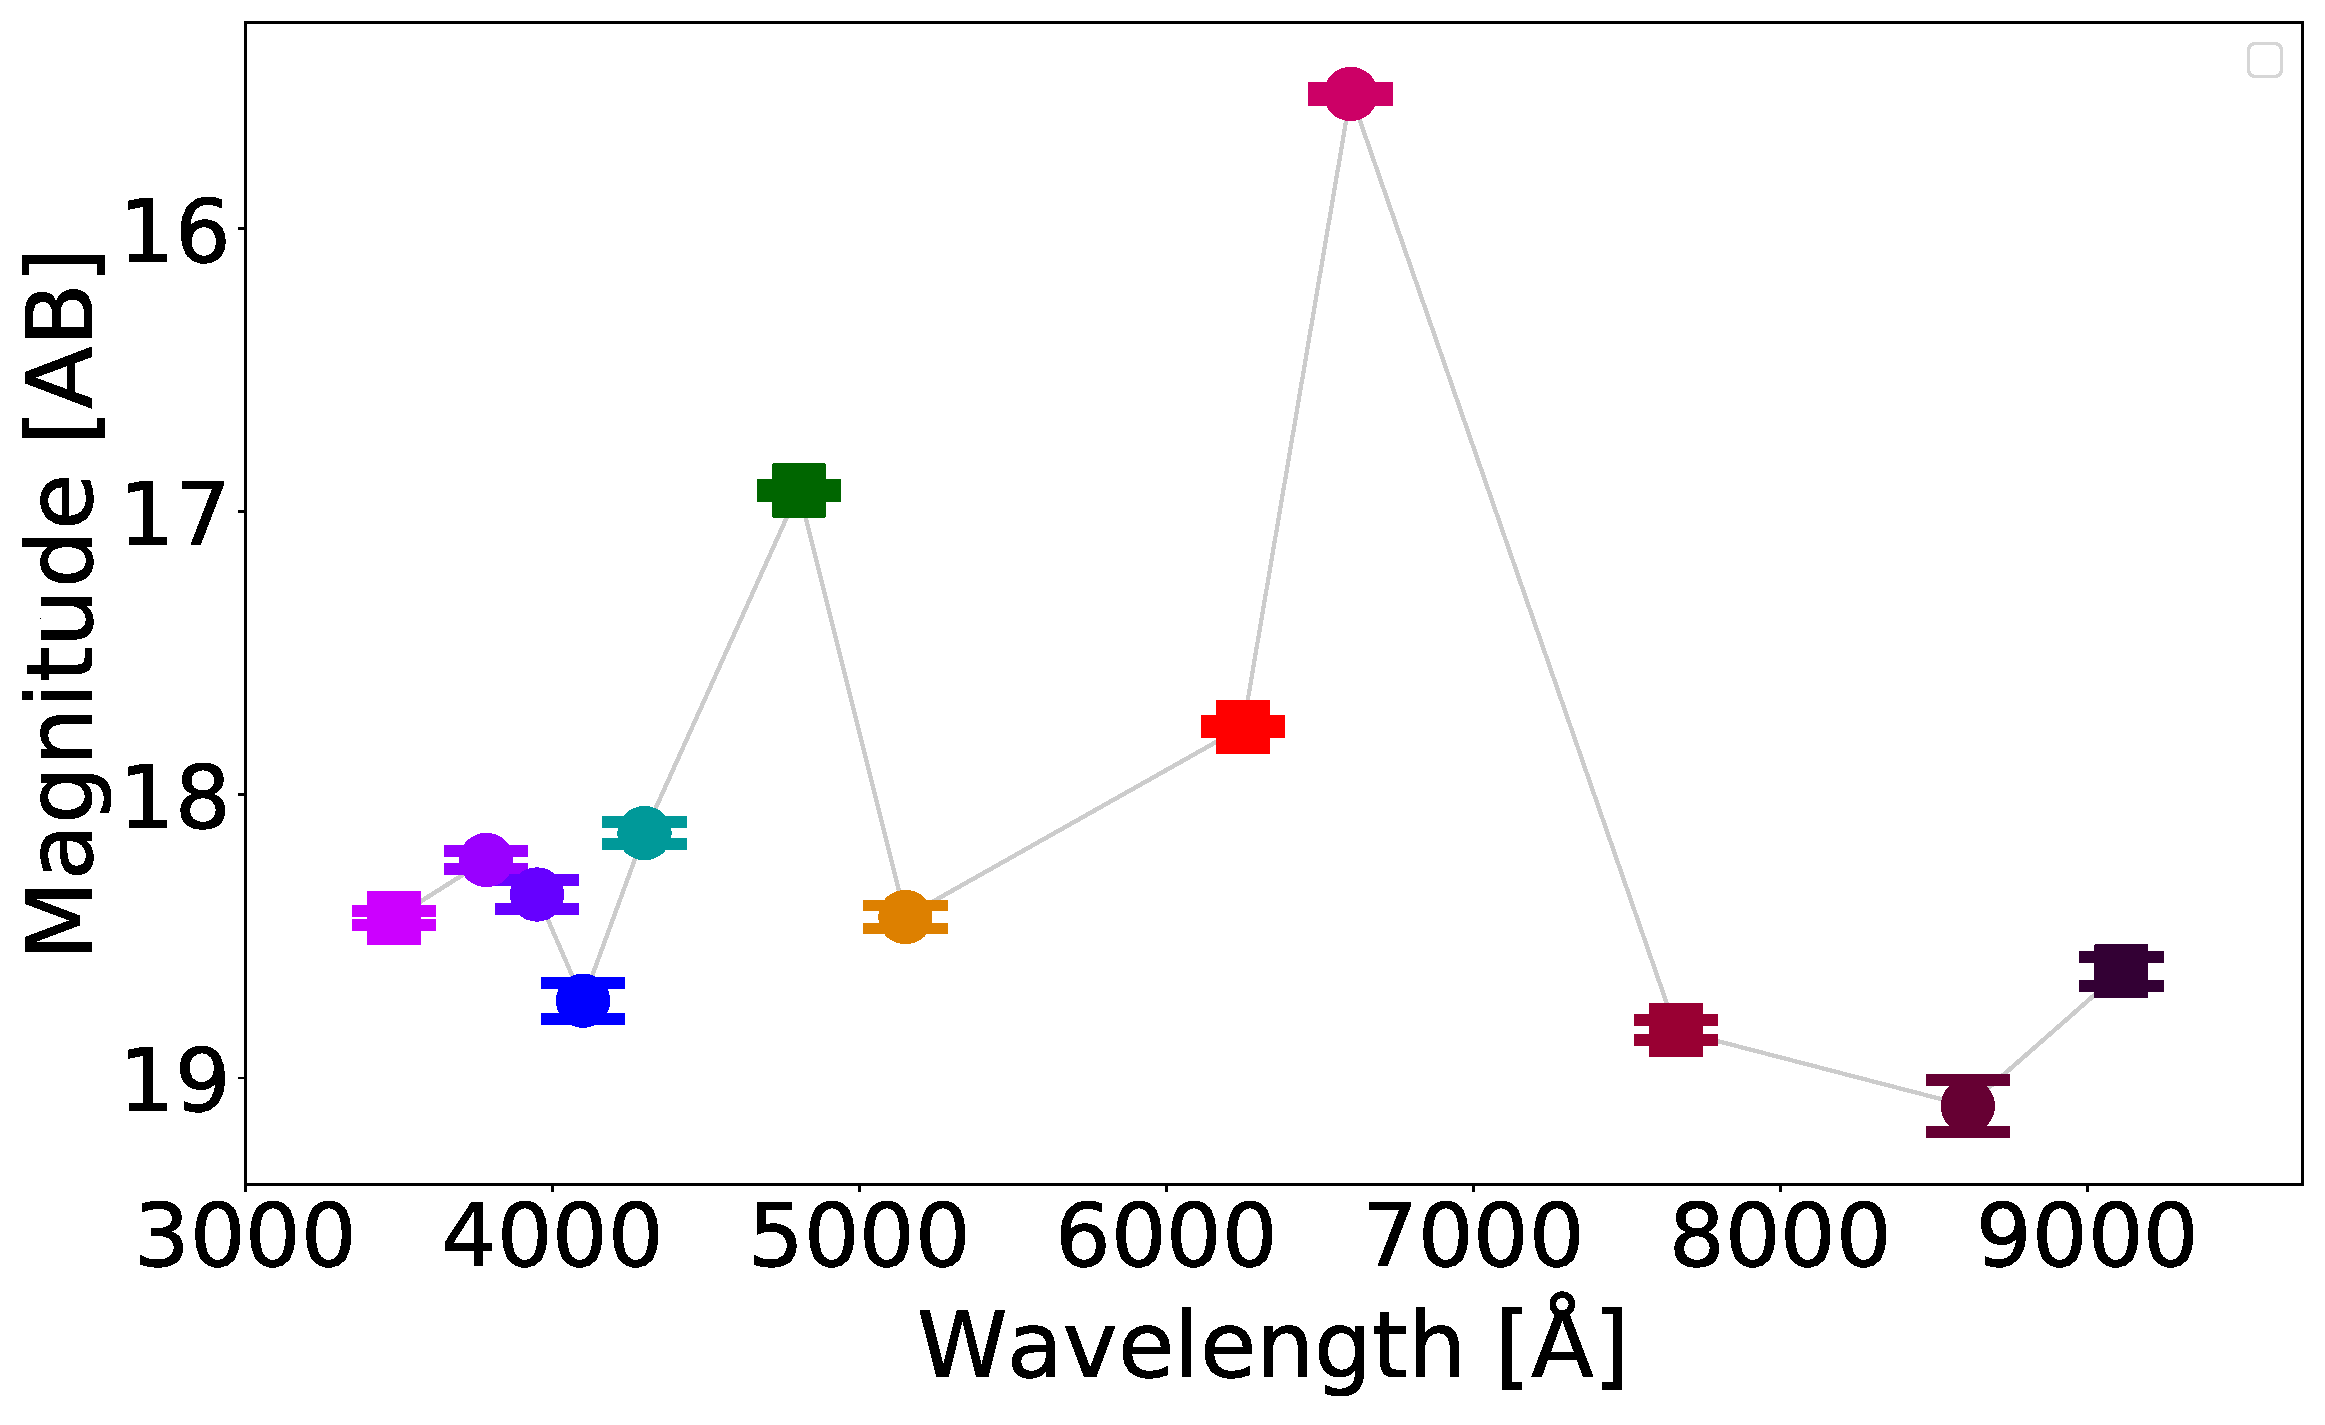
\includegraphics[width=0.3\linewidth, clip]{photopectrum_splus_MC0115-112627_aper.pdf} & \includegraphics[width=0.3\linewidth, clip]{photopectrum_splus_MC0115-112627_auto.pdf} & \includegraphics[width=0.3\linewidth, clip]{photopectrum_splus_MC0115-112627_petro.pdf} \\
\includegraphics[width=0.3\linewidth, clip]{photopectrum_splus_MC0115-147165_aper.pdf} & \includegraphics[width=0.3\linewidth, clip]{photopectrum_splus_MC0115-147165_auto.pdf} & \includegraphics[width=0.3\linewidth, clip]{photopectrum_splus_MC0115-147165_petro.pdf} \\
\includegraphics[width=0.3\linewidth, clip]{photopectrum_splus_MC0115-229578_aper.pdf} & \includegraphics[width=0.3\linewidth, clip]{photopectrum_splus_MC0115-229578_auto.pdf} & \includegraphics[width=0.3\linewidth, clip]{photopectrum_splus_MC0115-229578_petro.pdf} \\
\includegraphics[width=0.3\linewidth, clip]{photopectrum_splus_MC0115-308119_aper.pdf} & \includegraphics[width=0.3\linewidth, clip]{photopectrum_splus_MC0115-308119_auto.pdf} & \includegraphics[width=0.3\linewidth, clip]{photopectrum_splus_MC0115-308119_petro.pdf} \\

\end{tabular}
\end{table}

\begin{table}
\begin{tabular}{ccc}
\includegraphics[width=0.3\linewidth, clip]{photopectrum_splus_MC0115-350934_aper.pdf} & \includegraphics[width=0.3\linewidth, clip]{photopectrum_splus_MC0115-350934_auto.pdf} & \includegraphics[width=0.3\linewidth, clip]{photopectrum_splus_MC0115-350934_petro.pdf} \\
\includegraphics[width=0.3\linewidth, clip]{photopectrum_splus_MC0115-402039_aper.pdf} & \includegraphics[width=0.3\linewidth, clip]{photopectrum_splus_MC0115-402039_auto.pdf} & \includegraphics[width=0.3\linewidth, clip]{photopectrum_splus_MC0115-402039_petro.pdf} \\
\includegraphics[width=0.3\linewidth, clip]{photopectrum_splus_MC0116-015280_aper.pdf} & \includegraphics[width=0.3\linewidth, clip]{photopectrum_splus_MC0116-015280_auto.pdf} & \includegraphics[width=0.3\linewidth, clip]{photopectrum_splus_MC0116-015280_petro.pdf} \\
\includegraphics[width=0.3\linewidth, clip]{photopectrum_splus_MC0116-172101_aper.pdf} & \includegraphics[width=0.3\linewidth, clip]{photopectrum_splus_MC0116-172101_auto.pdf} & \includegraphics[width=0.3\linewidth, clip]{photopectrum_splus_MC0116-172101_petro.pdf} \\
\includegraphics[width=0.3\linewidth, clip]{photopectrum_splus_MC0133-025038_aper.pdf} & \includegraphics[width=0.3\linewidth, clip]{photopectrum_splus_MC0133-025038_auto.pdf} & \includegraphics[width=0.3\linewidth, clip]{photopectrum_splus_MC0133-025038_petro.pdf} \\
\end{tabular}
\end{table}




\end{document}